%\documentclass[preprint,10pt]{sigplanconf}
\documentclass[10pt]{sigplanconf}

\usepackage{times}


\usepackage{graphicx,url,color}
\usepackage[noend]{algpseudocode}
\usepackage{algorithmicx,algorithm}
\usepackage{listings}
\usepackage{paralist}
\usepackage{amsmath}
%\usepackage{caption}yes
\usepackage[skip=0pt]{subcaption}
%\usepackage[tight]{subfigure}
%\usepackage{eepic}
%\usepackage{dblfloatfix} % fix for bottom-placement of figure
%\usepackage{perpage}
\usepackage{balance}
\usepackage{xcolor}

%% $Id: genericmacros.tex,v 1.1 2008/11/06 22:41:17 eyahav Exp $
% Generic macros (nothing specific to this paper)

\usepackage{ifthen}
\usepackage{multirow}
%

%%%%%%%%%%%%%%%%%%%%%%%%%%%%%%%%%%%%%%%%%%%%%%%%%%%%%
%% Terminology                                     %%
%%%%%%%%%%%%%%%%%%%%%%%%%%%%%%%%%%%%%%%%%%%%%%%%%%%%%
\newcommand{\demonsmarker}{\textbf{\color{blue} DEMONS START HERE IF NOT EARLIER}}

%\newcommand{\scode}[1]{{ \texttt{#1}}}
%\newcommand{\sname}[1]{{\small \textsc{#1}}}

\newcommand{\TODO}[1]{{{\color{blue}{\bf #1}} }}
\newcommand{\TODOFN}[1]{ \footnote{{\bf #1}} }
\newcommand{\DONE}[1]{}
\newcommand{\COMMENT}[1]{}
\newcommand{\ie}{i.e.}
\newcommand{\eg}{e.g.}
%%% references definition
\newcommand{\lnref}[1]{Line~\ref{Ln:#1}}
\newcommand{\lemref}[1]{Lemma~\ref{Lm:#1}}
\newcommand{\figref}[1]{Figure~\ref{Fi:#1}}
\renewcommand{\algref}[1]{Algorithm~\ref{Al:#1}}
\newcommand{\defref}[1]{Definition~\ref{De:#1}}
\newcommand{\theref}[1]{Theorem~\ref{Th:#1}}
\newcommand{\tabref}[1]{Table~\ref{Ta:#1}}
\newcommand{\secref}[1]{Section~\ref{Se:#1}}
\newcommand{\secrefs}[2]{Sections~\ref{Se:#1}-\ref{Se:#2}}
\newcommand{\ssecref}[1]{Section~\ref{Se:#1}}
\newcommand{\appref}[1]{Appendix~\ref{Se:#1}}
\newcommand{\exref}[1]{Example~\ref{Ex:#1}}
\newcommand{\chapref}[1]{Chapter~\ref{Ch:#1}}
\newcommand{\equref}[1]{Equation~\ref{Eq:#1}}
\newcommand{\corref}[1]{Corollary~\ref{Co:#1}}

\newcommand{\lemlabel}[1]{\label{Lm:#1}}
\newcommand{\figlabel}[1]{\label{Fi:#1}}
\newcommand{\deflabel}[1]{\label{De:#1}}
\newcommand{\thelabel}[1]{\label{Th:#1}}
\newcommand{\tablabel}[1]{\label{Ta:#1}}
\newcommand{\seclabel}[1]{\label{Se:#1}}
\newcommand{\sseclabel}[1]{\label{Se:#1}}
\newcommand{\applabel}[1]{\label{Se:#1}}
\newcommand{\exlabel}[1]{\label{Ex:#1}}

%%\newtheorem{Examp}{Example}
\newtheorem{definition}{Definition}
%%% sectioning


\newcounter{programlinenumber}
\newenvironment{pgm}
     {\tt%
       \begin{tabbing}%
       123\=123\=123\=123\=123\=123\=123\=123\=123\=123\=123\=123\=\kill%
       \setcounter{programlinenumber}{0}%
     }
     {\end{tabbing}}
\newcommand{\nl}{\addtocounter{programlinenumber}{1}[\arabic{programlinenumber}] \> }
\newcommand{\nonl}{}%
\newenvironment{narrowpgm}
     {\tt%
       \begin{tabbing}%
       12\=12\=12\=12\=12\=12\=12\=12\=12\=12\=12\=12\=\kill%
       \setcounter{programlinenumber}{0}%
     }
     {\end{tabbing}}

\newenvironment{basenarrowpgm}
     {\tt%
       \begin{tabbing}%
       \=12\=12\=12\=12\=12\=12\=12\=12\=12\=12\=12\=12\=\kill%
       \setcounter{programlinenumber}{0}%
     }
     {\end{tabbing}}


\newenvironment{xbasenarrowpgm}
     {\tt%
       \begin{tabbing}%
       1\=1\=1\=1\=1\=1\=1\=1\=1\=1\=1\=1\=1\=\kill%
       \setcounter{programlinenumber}{0}%
     }
     {\end{tabbing}}

%% if statement
\newcommand{\ifthen}[3]{
 \left\{
      \begin{array}{ll}
        #2 & #1 \\
        #3 & {\rm otherwise}
      \end{array}
      \right.
 }

%% TO Allow writing the TR in the same source
\newboolean{TR}
\setboolean{TR}{false}
\ifthenelse{\boolean{TR}}{
\newcommand{\TrSelect}[2]{#1}
\newcommand{\TrOnly}[1]{#1}
\newcommand{\SubOnly}[1]{}
\newcommand{\TrOnlyInFootnote}[1]{#1}
\newcommand{\TrOnlyInTable}[1]{#1}}
{
\newcommand{\TrSelect}[2]{#2}
\newcommand{\TrOnly}[1]{}
\newcommand{\SubOnly}[1]{#1}
\newcommand{\TrOnlyInFootnote}[1]{}
\newcommand{\TrOnlyInTable}[1]{}}



%% General macros
\newcommand{\Set}[1]{\{ \; {#1} \; \}}
\newcommand{\vbar}{\; | \;}
\newcommand{\notIn}{\not\in}
\newcommand{\sizeof}[1]{|{#1}|}
%% \newcommand{\isDefined}{=_{def}}
\newcommand{\isDefined}{\triangleq}

\newcommand{\lt}{$<$}
\newcommand{\gt}{$>$}

%% tminus: "thin minus", with less space around it;
%% telem: "thin element"
\newcommand{\tminus}{\!\! - \!\!}
\newcommand{\telem}{\! \in \!}

%% stexttt: "small" texttt
\newcommand{\stexttt}[1]{{\small \texttt{#1}}}

\newcommand{\mathify}[1]{\mathord{\mbox{#1}}}
\newcommand{\italMathId}[1]{\mathify{\textit{\textrm{#1}}}}
\newcommand{\romanMathId}[1]{\mathify{\textup{\textrm{#1}}}}
\newcommand{\ttMathId}[1]{\mathify{\textup{\texttt{#1}}}}

\newcommand{\ttsub}[2]{${\ttMathId{#1}}_{#2}$}
\newcommand{\ttsup}[2]{${\ttMathId{#1}}^{#2}$}
\newcommand{\mttsub}[2]{{\ttMathId{#1}}_{#2}}
\newcommand{\twoarray[2]}{\begin{array}{l}  #1 \\ #2 \end{array}}
\newcommand{\subsubsubsection}[1]{\emph{#1}:}


\newcommand{\inred}[1]{{\color{red}{#1}}}
\newcommand{\newnote}[1]{\frameit{Note}{#1}}
\newcommand{\todo}[1]{\frameit{To-do}{#1}}
\newcommand{\microsec}{${\mu}$s}
\newcommand{\scode}[1]{{\small \texttt{#1}}}
\newcommand{\NULL}{\bot}


\newcommand{\clsm}{cLSM}
\newcommand{\leveldb}{LevelDB}
\newcommand{\hyperleveldb}{HyperLevelDB}
\newcommand{\rocksdb}{RocksDB}
\newcommand{\blsm}{bLSM}
\newcommand{\fdplus}{FD+}

\newcommand{\inote}[1]{}
\newcommand{\remove}[1]{}
\newcommand{\frameit}[2]{
    \begin{center}
    {\color{red}
    \framebox[3.3in][l]{
        \begin{minipage}{3in}
        \inred{#1}: {\sf\color{black}#2}
        \end{minipage}
    }\\
    }
    \end{center}
}

\newcommand{\comment}[1]{}
\newcommand{\eshcar}[1]{\noindent{\textcolor{violet}{\{{\bf eshcar:} \em #1\}}}}
%\newcommand{\eurosys}[2]{{\color{red}\inred{#1}: {\color{violet}#2}}}
\newcommand{\eurosys}[2]{#2}
\newcommand{\guy}[1]{\noindent{\textcolor{blue}{\{{\bf guy:} \em #1\}}}}

\newcommand\keywordstyle{\rmfamily\bfseries\upshape}
\newcommand\operatorstyle{\rmfamily\mdseries\upshape}
\newcommand\typestyle{\rmfamily\mdseries\upshape}
\newcommand\functionstyle{\rmfamily\mdseries\scshape}
\newcommand\identifierstyle{\rmfamily\mdseries\itshape}

\newcommand{\para}[1]{\vspace{3pt}\noindent\textbf{\textit{#1}}}

\newcommand\addkeywords[1]{%
  \lstset{morekeywords=[1]{#1}}}

\newcommand\addoperators[1]{%
  \lstset{morekeywords=[2]{#1}}}

\newcommand\addtypes[1]{%
  \lstset{morekeywords=[3]{#1}}}

\newcommand\addfunctions[1]{%
  \lstset{morekeywords=[4]{#1}}}

\newcommand{\tuple}[1]{\ensuremath{\left\langle {#1} \right\rangle}}
\algnewcommand{\algorithmicgoto}{\textbf{goto}}%
\algnewcommand{\Goto}[1]{\algorithmicgoto~\ref{#1}}%


%\newtheorem{definition}{Definition}%[section]
%\newtheorem{theorem}{Theorem}
%\newtheorem{lemma}[theorem]{Lemma}
%\newtheorem{corollary}[theorem]{Corollary}
%\renewcommand\footnotesize{\small}
%\setlength{\textfloatsep}{0.15in}
%\setlength{\abovecaptionskip}{10pt}
%\setlength{\belowcaptionskip}{-2pt}

\newcommand{\key}{\italMathId{key}}
\newcommand{\ts}{\italMathId{ts}}
\newcommand{\val}{\italMathId{val}}
\newcommand{\ptr}{\italMathId{ptr}}
\newcommand{\LimitSize}{\italMathId{LimitSize}}
\newcommand{\OK}{\italMathId{OK}}
\newcommand{\FULL}{\italMathId{FULL}}
\newcommand{\NONE}{\italMathId{NONE}}

\newcommand{\negspace}{\vspace{-0.5\baselineskip}}

\newcommand{\Idit}[1]{{\bf [[Idit: #1]]}}
\newcommand{\omitit}[1]{}

\begin{document}
% --- Author Metadata here ---
\conferenceinfo{EuroSys '15}{April 21--24, 2015, Bordeaux, France}
\copyrightyear{2015}
\copyrightdata{978-1-4503-3238-5/15/04}
\doi{2741948.2741973}
% --- End of Author Metadata ---

\title{Scaling Concurrent Log-Structured Data Stores}
%\remove{
\authorinfo{Guy Golan-Gueta}{Yahoo Labs\\Haifa,
Israel}{ggolan@yahoo-inc.com}
\authorinfo{Edward Bortnikov}{Yahoo Labs\\Haifa,
Israel}{ebortnik@yahoo-inc.com}
\authorinfo{Eshcar Hillel}{Yahoo Labs\\Haifa,
Israel}{eshcar@yahoo-inc.com}
\authorinfo{Idit Keidar}{Technion, Yahoo Labs\\Haifa,
Israel}{idish@ee.technion.ac.il}
%\authorinfo{Paper \#96 ; 13 pages}{}{}
%}
\remove{
\numberofauthors{4}
\author{
 \alignauthor Guy Golan-Gueta\\
   \affaddr Yahoo Labs\\
   \affaddr Haifa, Israel\\
   \email{ggolan@yahoo-inc.com}
 \alignauthor Edward Bortnikov\\
    \affaddr Yahoo Labs\\
    \affaddr Haifa, Israel\\
    \email{ebortnik@yahoo-inc.com}
  \alignauthor Eshcar Hillel\\
    \affaddr Yahoo Labs\\
    \affaddr Haifa, Israel\\
    \email{eshcar@yahoo-inc.com}
\alignauthor Idit Keidar\\
   \affaddr Technion\\
   \affaddr Haifa, Israel\\
   \email{idish@ee.technion.ac.il}
}
}

\maketitle

\begin{abstract}

Log-structured data stores (LSM-DSs) are widely accepted as the state-of-the-art implementation of key-value stores. They replace random disk writes with sequential I/O, by accumulating large batches of updates in an in-memory data structure and merging it with the on-disk store in the background. While LSM-DS implementations proved to be highly successful at masking the I/O bottleneck, scaling them up on multicore CPUs
remains a challenge. This is nontrivial due to their often rich APIs, as well as the need to coordinate the RAM access with the background I/O.

We present \clsm, an algorithm for scalable concurrency in LSM-DS, which exploits multiprocessor-friendly data structures and non-blocking synchronization. \clsm\ supports a rich API, including consistent snapshot scans and general non-blocking read-modify-write operations.

We implement \clsm\ based on the popular \leveldb\  key-value store, and evaluate it using intensive synthetic workloads as well as ones from production web-serving applications. Our algorithm outperforms state of the art LSM-DS implementations, improving throughput by 1.5x to 2.5x. Moreover, \clsm\ demonstrates superior scalability with the number of cores (successfully exploiting twice as many cores as the competition).


%Log-structured data stores (LSM-DSs) are widely accepted as the state-of-the-art implementation of NoSQL key-value stores. They replace random disk writes with sequential I/O, by accumulating large batches of updates in an in-memory data structure and merging it with the on-disk store in the background. While LSM-DS implementations proved to be highly successful with masking the I/O bottleneck, their main challenge is scaling up on multicore CPUs. This is nontrivial due to their often rich APIs, as well as the need to coordinate the RAM access with the background I/O.
%
%We present \clsm, (pronounced Colosseum), an algorithm for scalable concurrency in LSM-DS, which exploits multiprocessor-friendly data structures and non-blocking synchronization in order to overcome the vertical scalability challenge. It supports a rich API, including snapshots, iterators, and general non-blocking read-modify-write operations. Our algorithm is non-blocking in all scenarios that do not involve access to disk.
%
%We implement \clsm\ based on the popular \leveldb\ key-value store, and evaluate it extensively using intensive synthetic workloads as well as ones from production Web-serving applications. Our algorithm conclusively outperforms state of the art LSM-DS implementations, improving throughput by 1.5x to 2.5x, and reducing latency by a similar factor. Moreover, \clsm\ demonstrates superior scalability with the number of cores (successfully exploiting at least twice as
%many cores as the competition).

\negspace
\end{abstract}

\section{Introduction}
\label{sec:intro}

%key-value databases
Over the last decade,  \emph{key-value stores} have become prevalent
for real-time serving of Internet-scale data~\cite{Bigtable2006}. Gigantic  stores managing billions of items
serve Web search indexing~\cite{Percolator2010}, messaging~\cite{FBMessaging2012}, personalized media,
and advertising~\cite{PNUTS2008}. A key-value store is essentially a persistent map with atomic get and put
operations used to access data items identified by unique keys.
%Typical response times feature low milliseconds per request within a datacenter~\cite{RocksDB}.
Modern  stores also support consistent snapshot scans and range queries for online analytics.

%LSM-stores
In write-intensive environments, key-value stores are commonly implemented  as
\emph{Log-Structured Merge Data Stores (LSM-DSs)}~\cite{leveldb,Bigtable2006,PNUTS2008,hbase,Lakshman2010,RocksDB,BLSM2012}
(see Section~\ref{sec:background}). The main centerpiece behind such data stores is absorbing large batches of writes
in a RAM data structure that is merged into a (substantially larger) persistent data store upon spillover.
This approach masks persistent storage latencies from the end user, and increases throughput by performing I/O sequentially.
%In addition, LSM-DSs are friendly to SSD storage, which
%sustains a limited number of rewrites per disk block, and therefore does not suffer random updates.
A major bottleneck of such data stores is their limited in-memory concurrency,
%especially for writes,
which, as we show in Section~\ref{sec:eval}, restricts their vertical scalability on multicore servers. In the past,
this was not a serious limitation, as large Web-scale servers did not harness high-end multi-core hardware.
Nowadays, however, servers with more cores have become cheaper, and 16-core machines commonplace
in production settings.

Our goal in this work is to improve the scalability of state-of the art key-value stores on multicore servers.
We focus on a data store that runs on a single multicore machine, which is often the basic building block
for a distributed database that runs on multiple machines (e.g.,~\cite{Bigtable2006,PNUTS2008}). Although
it is possible to scale up by further partitioning the data and running multiple LSM-DS's on the same machine,
there are significant advantages to consolidation~\cite{hbaseRegionArch}; see more detailed discussion in Section~\ref{sec:background}. We therefore strive to
scale up a single LSM-DS by maximizing its parallelism.

We present (in Section~\ref{sec:algorithm}) {\clsm}, \remove{-- pronounced Colosseum --} a scalable  LSM-DS
algorithm optimized for multi-core machines. We implement  \clsm\ in the framework of the popular \leveldb~\cite{leveldb}
library (Section~\ref{sec:impl}), and evaluate it extensively (Section~\ref{sec:eval}), showing better scalability and
1.5x to 2.5x performance improvements over the state-of-the art.

\subsection*{Contributions}

This paper makes the following contributions:

\para{Non-blocking synchronization.}
{\clsm} overcomes the scalability bottlenecks incurred in previous works~\cite{leveldb,Hyperdex2012} by eliminating
blocking during normal operation. It never explicitly blocks get operations, and
only blocks puts for short periods of time before and \eurosys{A1}{after batch
I/Os.
%While quite a few previous works have used non-blocking synchronization at the
% data structure level~\cite{Herlihy2008}, we are not aware of any previous work that improved full-system performance using this approach.
}
% Consequently, in the absence of physical disk access, \clsm\ is non-blocking (lock-free).

% rich api
\para{Rich API.}
Beyond atomic put and get operations, \clsm\ also supports consistent
snapshot scans, which can be used to provide range queries.  These are
important for  applications such as online analytics~\cite{Bigtable2006}, and multi-object transactions~\cite{Omid2014}.
In addition, \clsm\ supports fully-general non-blocking atomic \emph{read-modify-write} (RMW) operations. We are not aware of any existing lock-free support for such operations in today's key-value stores. Such operations are useful, e.g., for multisite update reconciliation~\cite{PNUTS2008,Dynamo07}.

\para{Generic algorithm.} %{\color{blue}TODO}
Our algorithm for supporting puts, gets, snapshot scans, and range queries is decoupled from any specific implementation of the LSM-DS's main building blocks, namely the in-memory component (a map data structure), the disk store,  and the merge process that integrates the former into the latter.
Only our support for atomic read-modify-write requires a specific implementation of the in-memory component
as a skip-list data structure.
This allows one to readily benefit from numerous optimizations of other components
(e.g., disk management~\cite{RocksDB}) which are orthogonal to our contribution.

\para{Implementation.}
We implement a working prototype of {\clsm} based on {\leveldb}~\cite{leveldb}, a state-of-the-art key-value store.
Our implementation supports the full functionality of {\leveldb}
\eurosys{I4}{and inherits its core modules (including disk and cache management),
and therefore benefits from the same optimizations.}

\para{Evaluation.}
We compare \clsm's performance to {\leveldb} and three additional open-source key-value stores,
HyperLevelDB~\cite{Hyperdex2012},  bLSM~\cite{BLSM2012}, and RocksDB~\cite{RocksDB}, on production-grade multi-core hardware.
We evaluate the systems under large-scale intensive synthetic workloads as well as production workloads from
a web-scale system serving personalized content and ad recommendation products.

In our experiments, {\clsm} achieves performance improvements ranging between 1.5x and 2.5x
over the best competitor, on a variety of workloads.
\clsm's RMW operations are also twice as fast as a popular implementation based on lock striping~\cite{GrayTP1993}.
%Across all workloads,
Furthermore, \clsm\ exhibits superior scalability, successfully utilizing at least twice as many threads, and also
benefits more from a larger RAM allocation to the in-memory component.
%Finally, \clsm's memory-based put and get operations are unaffected by background disk snapshot scans.
%Finally, {\clsm} efficiently separates the real-time and analytics workloads -- its per-CPU performance is unaffected
%by background disk scans.
%Our results manifest consistently across magnetic and flash storage.

%We evaluate the performance of our implementation on several synthetic and real-life workloads.
%Our evaluation shows that {\clsm} provides scalable read and write operations.
%Furthermore, the evaluation indicates that our {\clsm} implementation outperforms existing state of the art implementations of concurrent LSM-stores.
%{\color{blue}TODO: explain that we benefit from the cache of the disk).}
%{\color{blue}TODO: mention almost lock-free (and the impact on performance).}


\section{Architecture Principles}
\label{sec:background}

%Prior to getting into the details of our algorithm,

We overview our design choices, as motivated by today's leading key-value store implementations.
We discuss their API, approaches to scaling them, and the LSM approach to data management.

\subsection{Data Model and API}
\label{ssec:kvs}

In key-value stores~\cite{Bigtable2006,PNUTS2008,hbase}, the data is comprised
of items ({\em rows}) identified by unique keys. A row value is a (sparse) bag of attributes called {\em columns}.
The internal structure of data items is largely opaque for the rest of our discussion.
%Co-accessed columns (typically used by the same application) can be aggregated
% in {\em column families} to optimize access.

The basic API of a key-value store includes \emph{put} and \emph{get} operations to store and retrieve values by their keys.
Updating an item is cast into putting an existing key with a new value, and deleting
one is performed by putting a \emph{deletion marker}, $\NULL$, as the key's value.

To cater to the demands of online analytics applications (e.g.,~\cite{Percolator2010}), key-value stores typically
support \emph{snapshot scans}, which provide consistent read-only views of the data. A scan allows the user to acquire a
snapshot of the data (\emph{getSnap}), from which the user can iterate over
items in lexicographical order of their keys by applying \emph{next} operations.

Geo-replication scenarios drive the need to reconcile conflicting replicas.
This is often done through vector clocks~\cite{Dynamo07}, which require the key-value store
to support conditional updates, namely, atomic read-modify-write
operations.

\subsection{Scalability in Distributed Key-Value Stores}
Distributed key-value stores achieve scalability by sharding data into units called {\em partitions}
(also referred to as \emph{tablets}~\cite{Bigtable2006, PNUTS2008} or \emph{regions}~\cite{hbase}).
%There is a variety of methods to shard data by
%key, range and hash partitioning being most notable~\cite{GrayTP1993}.
%
Partitioning provides {\em horizontal scalability} -- stretching the service across multiple servers.
%Production web-scale stores are comprised of thousands of such servers~\cite{Bigtable2006}, each managing
%dozens of partitions~\cite{hbaseRegionArch}.
Nevertheless, there are penalties associated with having many partitions, as argued in~\cite{hbaseRegionArch}:
First, the data store's consistent snapshot scans do not span multiple partitions. Analytics applications that
require large consistent scans are forced to use costly transactions across shards.
%Second, the system-level meta-data increases with the number of partitions, and can become a bottleneck.
%
Second, this requires a system-level mechanism for managing partitions~\cite{Bigtable2006,PNUTS2008,hbase}, whose meta-data size depends on the number of partitions, and can become a scalability bottleneck.




The complementary approach of
increasing the serving capacity of each individual partition is called
\emph{vertical scalability}. First, this necessitates optimizing the speed of I/O-bound operations.
The leading approach to do so, especially in write-intensive settings,
is  LSM  (discussed in Section~\ref{ssec:lsm}), which
%replaces random disk accesses with sequential I/O,
effectively eliminates the disk bottleneck.
Once this is achieved, the rate of in-memory operations becomes paramount (as we show in Section~\ref{sec:eval}).
Increasing this rate is the challenge we focus on in this paper.

We argue here that we can improve performance while reducing the number of partitions,
which in turn allows for larger snapshot scans and reduces meta-data size.
To illustrate this point, Figure~\ref{fig:production_partitions} shows sample results from our experiments (the experiment
setup is detailed in Section~\ref{sec:eval}). In this example, we evaluate {\clsm\/} with one big partition
versus {\leveldb\/} and {\hyperleveldb\/} with four small partitions, where each small partition's workload
is based on a distinct production log, and the big partition is the union thereof. Each of the small partitions is served
by a dedicated one quarter of the thread pool (resource separation), whereas the big partition is served by all
worker threads (resource sharing).
We see that {\clsm\/}'s improved concurrency control scales better than partitioning, achieving a peak throughput of above 1 million operations/sec -- approximately 25\% above the competition.


\begin{figure}[t]
\centerline{
{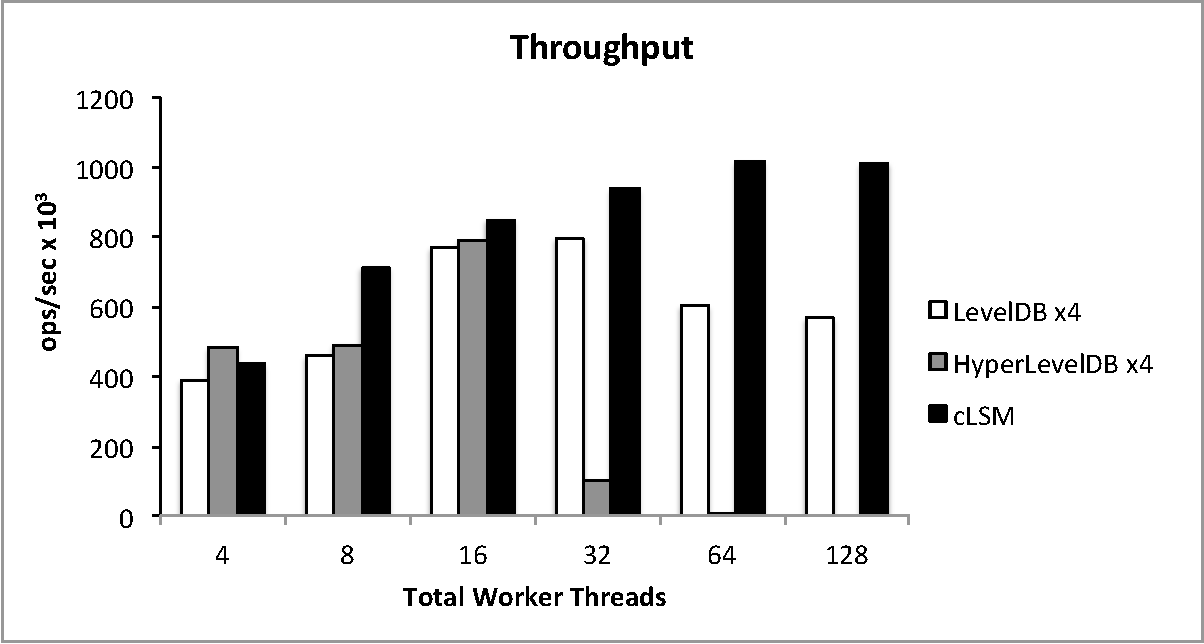
\includegraphics[width=\columnwidth]{Figures/prod4Partitions.pdf}}
}
\caption{\bf{Comparing two approaches to scalability with production workload.
The resource-isolated configuration exercises {\leveldb\/} and {\hyperleveldb\/} with
4 separate partitions, whereas the resource-shared configuration evaluates {\clsm\/} with
one big partition. }}
\label{fig:production_partitions}
\end{figure}


\remove{
One way to boost vertical scalability is keep partitions small, which reduces the need for concurrency control.
However, this approach also introduces new limitations. First, high partitioning granularity erodes the magnitude
of bulk disk operations performed by the LSM-DS merge function, thus adversely impacting the I/O
bottleneck~\cite{hbaseRegionArch}. In addition, it impedes sharing the server's resources (e.g., buffer
cache) across the partitions. We therefore strive to achieve vertical scalability by exploiting concurrency,
rather than by highly granular data partitioning.
}

\remove{
These phenomena are
manifested in the evaluation of our concurrent
algorithm over a complete instance of the database versus competitors that
utilize partitioning of the data (Section~\ref{sec:realworkloads}).
%Secondly, it puts the database's metadata service under strain.
%
On the semantic side, the atomicity of large scans across multiple partitions
(even on a single machine) can be addressed only via a
transactional processing layer~\cite{Percolator2010, Omid2014}, which is beyond
the scope of this work.
}

\subsection{Log-Structured Merge}
\label{ssec:lsm}

Disk access is a principal bottleneck in storage systems,
and remains a bottleneck even with today's
SSDs~\cite{Tanenbaum:2014:MOS,RocksDBBenchmarks,Wu:2012:AWB}. Since reads are often effectively masked by
caching, significant emphasis is placed on improving write throughput and latency~\cite{Tanenbaum:2014:MOS}.
It is therefore not surprising that log-structured merge solutions~\cite{O'Neil1996}, which batch writes  in memory
and merge them with on-disk storage in the background, have become the de facto
choice for today's leading key-value stores~\cite{Bigtable2006, FBMessaging2012, leveldb, RocksDB, Hyperdex2012, BLSM2012}.

An LSM data store organizes data in a series of components of increasing sizes, as illustrated in Figure~\ref{fig:tri}.
The first component, $C_m$, is an in-memory sorted
map that contains most recent data. The rest of the
components $C_1, \ldots, C_n$ reside on disk. For simplicity, in the context of
this work, they are perceived as a single
component, $C_d$.
An additional  important building block is the
\emph{merge} procedure, (sometimes called \emph{compaction}), which incorporates the contents of the memory component
into the disk, and the contents of each component into the next one.



\remove{
The choice of $C_m$'s size is affected by the merge procedure's performance.
On the one hand, $C_m$ should not be too big, to allow the merge to complete
fast and release the buffer for future use. On the other hand, it should not be too
small, to avoid frequent read/write spikes that access the same data many times
and waste the potential of sequential I/O~\cite{hbaseRegionArch}.
}


\remove{
In order to differentiate the interface of the internal map data structure from
that of the entire LSM-DS, we refer to the corresponding functions of the in-memory data structure
as \scode{insert} and \scode{find}.
%More precisely, the in-memory data structure supports at least the following two operations:
\begin{description}
\item [\scode{insert(k,v)}] -- inserts the key-value pair $(k,v)$ into the map.
If $k$  exists, the value associated with it is over-written.
A key is removed by inserting a $\NULL$ value.
\item[\scode{find(k)}] -- returns a value $v$ such that
 the map contains an item $(k,v)$, or $\NULL$ if no such value exists.
\end{description}
}

A put operation inserts an item into the main memory
component $C_m$, and logs it in a sequential file for recovery
purposes. Logging can be configured to be synchronous (blocking) or asynchronous
(non-blocking). The common default is asynchronous logging, which avoids waiting
for disk access, at the risk of losing some recent writes in case of a crash.

When $C_m$ reaches its size limit, which can be hard or soft, it is merged with
component $C_d$, in a way reminiscent of merge sort: The items of both $C_{m}$ and $C_{d}$, %or sub-ranges thereof,
are scanned and merged. %in memory buffers.
The new merged component
is then migrated to disk in bulk fashion, replacing the old component.
When considering multiple
disk components, $C_m$ is merged with component $C_1$.
Similarly, once a disk component $C_{i}$ becomes full its data is migrated to the
next component $C_{i+1}$.
Component merges are
%often referred to as \emph{compaction}, and are performed as
%background processes.
%Size management is done in a wrapper of the in-memory component, with a simple counter
%increment and check. Size limit can be hard or soft.
%
%The merge function is executed in a series of steps -- each step spans a key
% range.
%It is
executed in the background as an automatic maintenance service.


The get operation may require going
through multiple components until the key is found. But when get operations are
applied mostly to recently inserted keys, the search is completed in $C_m$.
Moreover, the disk component utilizes a large RAM cache. Thus, in workloads
that exhibit locality, most requests that do access  $C_{d}$ are satisfied from RAM
as well.

During a merge, the memory component becomes immutable,
at which point it is denoted
as $C'_m$. To allow put operations to be executed while rolling the merge, a
 new memory component $C_m$ then becomes available for updates (see
Figure~\ref{fig:comp}).
The put and get operations access the
components through three global pointers: pointers $P_m$ and $P'_m$ to the
\emph{current} (mutable) and \emph{previous} (immutable) memory components, and
pointer $P_d$ to the disk component. When the merge is complete, the previous
memory component is discarded. Allowing multiple puts and gets to be executed
in parallel is discussed in the sequel.

\begin{figure*}
  \centering
  \begin{subfigure}[t]{0.43\textwidth}
   \center
{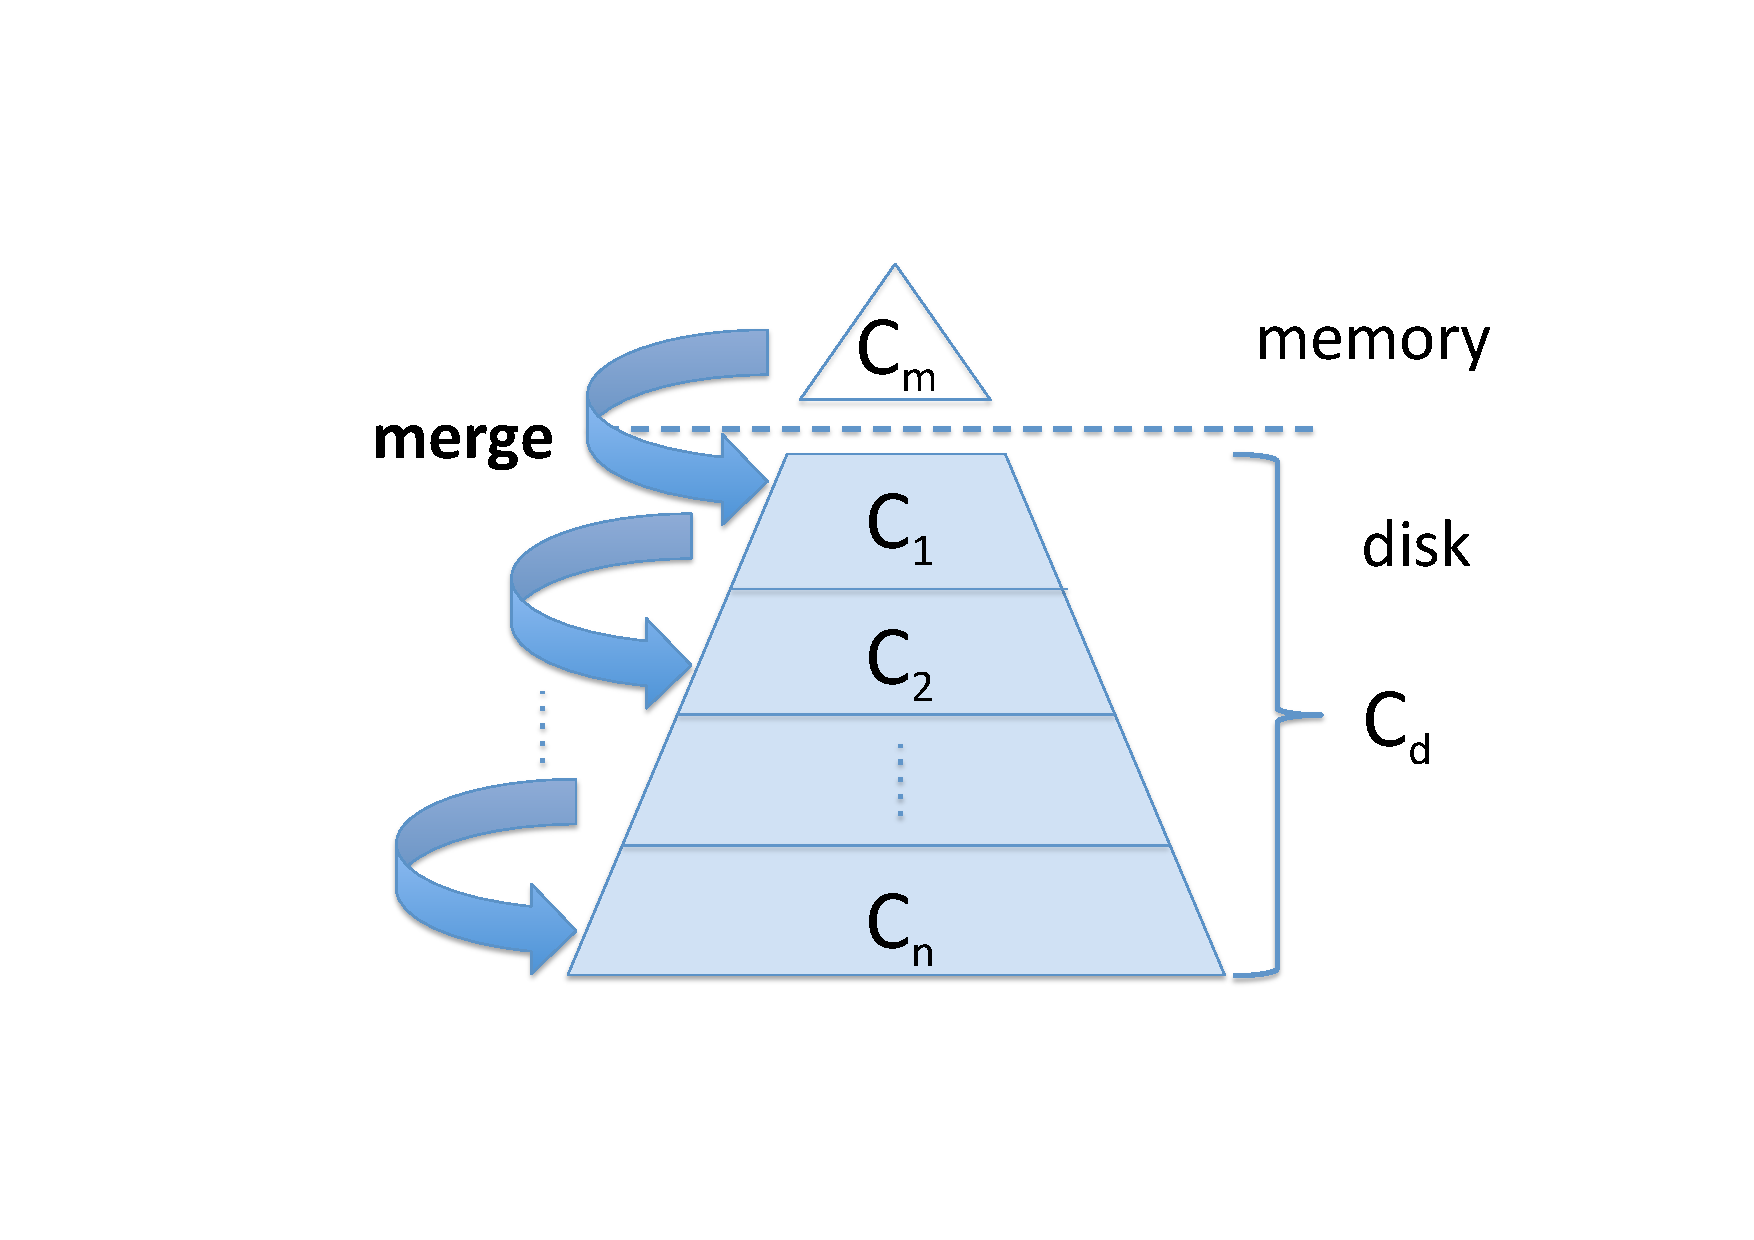
\includegraphics[width=0.6\textwidth,clip, trim =180 100 125 130]{Figures/triangle.pdf}} \caption{LSM-DS consists of a small memory component, and a large disk component
 comprised of a series of components of increasing sizes.}
               \label{fig:tri}
  \end{subfigure}%
  \hspace{0.1\textwidth}
  \begin{subfigure}[t]{0.43\textwidth}
   \center
{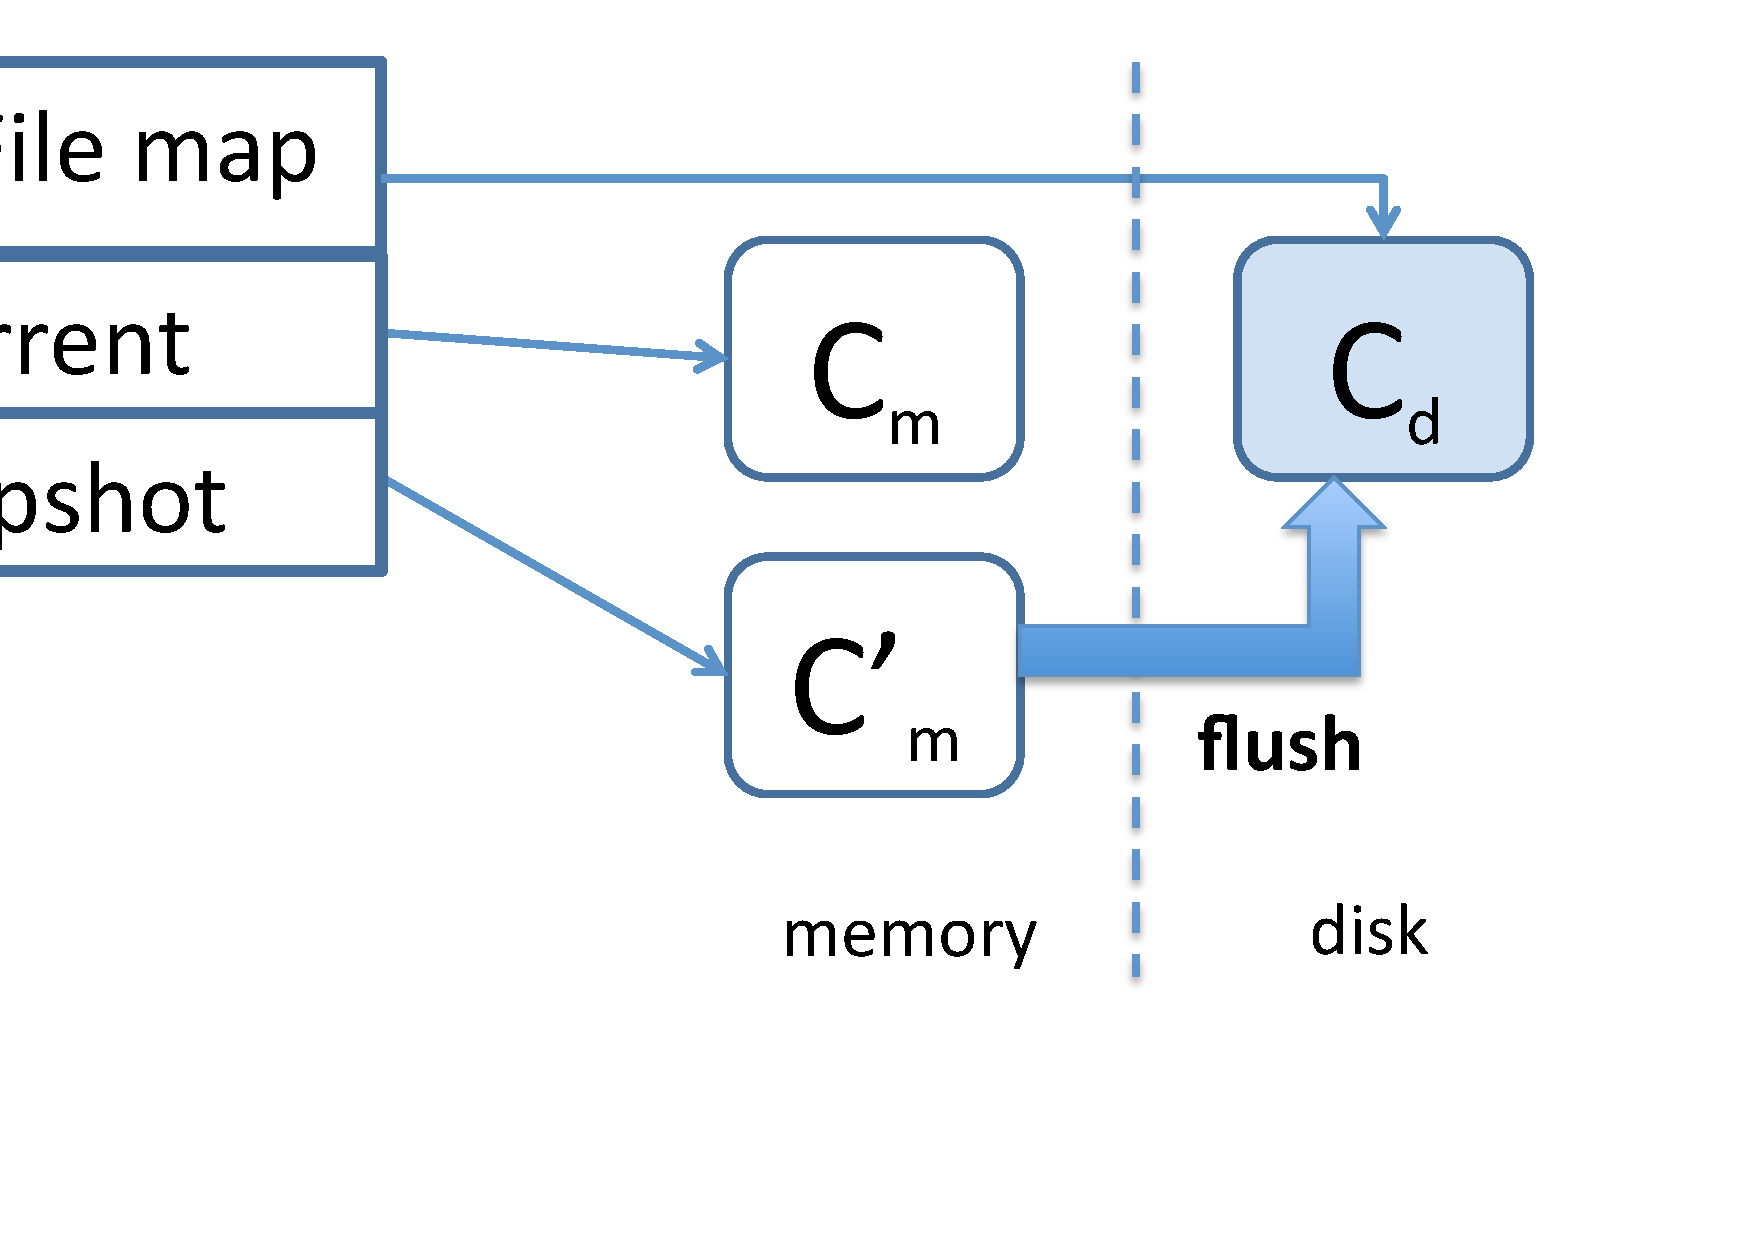
\includegraphics[width=0.6\textwidth,clip, trim =40 100 100 25]{Figures/architecture.pdf}} \caption{Global pointers $P_m$ to current (mutable) memory component
$C_m$, $P'_m$ to previous (immutable) memory component $C_m^{'}$, and $P_d$ to
disk component $C_d$. Merge incorporates  $C_m^{'}$ into $C_d$, while new
items are added to $C_m$.}
               \label{fig:comp}
  \end{subfigure}%
  \caption{\bf LSM-DS architecture.}
\label{fig:architecture}
\end{figure*} 
%\section{Algorithm}
\label{sec:algorithm}

\guy{working on this section}



\subsection{Shared Components}

Each component $c_i$ is an \emph{ordered set} of tuples $\tuple{\key,\ts,\val}$
where $\key$ is a key, $\ts$ is a timestamp, and $\val$ is a value.
The timestamp of a tuple $T$ represents the time when $T$ was added to the LSM-tree;
our algorithm ensures that each tuple has a unique timestamp.


\paragraph{Order of Tuples.}
We write $\leq_i$ to denote the order of the tuples in component $c_i$;
this order is used for implementing lookups, snapshots and the iteration functionality (described later).  
Each order $\leq_i$ satisfies the following conditions:
~(i) tuples with different keys are ordered according to a total order of the keys (defined by the client of the LSM-Tree);
~(ii) tuples with identical keys are ordered according to their timestamps.
In other words, if $\tuple{\key,\ts,\val} \leq_i  \tuple{\key',\ts',\val'}$ then either $\key < \key'$ or $\key = \key' \wedge \ts \leq \ts'$.

\paragraph{In-memory Components.}
The in-memory components are implemented as standard (ram-based) data structures.
An in-memory component supports the following functionality
\begin{itemize}
  \item The method \emph{insert} is used to add new tuples to the component.
  Normally, an invocation of \emph{insert($\tuple{\key,\ts,\val}$)} adds the tuple $\tuple{\key,\ts,\val}$ and returns $\OK$.
  Such invocation fails if the component already consumes (ay least) $\LimitSize$ bytes of memory
  ($\LimitSize$ is a numeric parameter defined by the client of the LSM-Tree),
  in this case the the tuple is not added and the method returns $FULL$ (an indication that new tuples cannot be added to this component).
  %
  \item The method \emph{get} is used to read a tuple that belongs to a specific timestamp.
  An invocation of \emph{get($\key,\ts$)} returns the maximal tuple $\tuple{k,t,v}$ such that $k=key$ and $t \leq ts$;
  if such a tuple does not exist, it returns $\NONE$.
  %
  \item \emph{Iterator}: enables traversing over all the tuples in the order defined by $\leq_i$.
  %
  \item \emph{Thread safety}:
  Several threads are permitted to simultaneously use the component:
  but each method invocation appears to execute atomically (as defined in~\cite{xxxx}).
  The iterator provides \emph{weak-consistency} (as in~\cite{xxx}):
  it returns tuples reflecting the state of the component at some point at or since the beginning of the iteration.
\end{itemize}

Our in-memory components are similar to the $leveldb$'s in-memory components.
But, in contrast to $leveldb$, we permit parallel executions of several \emph{insert} operations
(this enables our algorithm to provide scalable write-operations).

We have implemented the in-memory components by using the lock-free ordered-skip-list from~\cite{xxxx}
(based on the algorithm presented in \cite{xxx}).
Our implementation relies on the fact that this skip-list's iterator provides \emph{weak-consistency} as long as elements are never removed from the skip-list
(our algorithm does not remove elements from a component while it is being used).

In-memory components with the above functionality can be implemented
(in a straightforward way) by relying of other concurrent data structures (e.g.,~\cite{xxxx,xxxx}).
\TODO{GG: consider to add details (maybe in an appendix).}
%The above functionality can be realized, in a straightforward way, by relying of several other concurrent data structures, for example \cite{xxx}.

\paragraph{Disk-Based Components.}
The disk-based components are implemented as data structures that store the content of the tuples in the file-system.
A disk-based component is a read-only data structure: it is never updated after its creation.
It supports the method \emph{get} and an iterator (exactly as in the in-memory component).
For a disk-based component, thread-safety is simple since it is a read-only data structure.

In our implementation we have used the disk-based components  from the $\leveldb$ implementation.
%This enable us to use the "merge" (TBD) implemented in $\leveldb$.

%TODO: caching ?

\paragraph{Components Vector.}
The \emph{components vector} is a shared object that represents a vector of pointers $\tuple{p_1,\ldots,p_k}$
where each $p_i$ points to a shared component (denoted by $\overline{p_i}$).
%
For every $i < j$, the tuples in $\overline{p_i}$ are more recent than the tuples in $\overline{p_j}$
(that is, the timetags in $\overline{p_i}$ are larger than the ones in $\overline{p_j}$).

%The first component $\overline{p_1}$ is always an in-memory component, all new tuples are inserted to $\overline{p_1}$;
%the subsequent components $\overline{p_2},\ldots,\overline{p_k}$ are read-only.
%%
%Normally $\overline{p_2},\ldots,\overline{p_k}$ are disk-based components;
%only when the merge-process is executing $\overline{p_2}$ may be an in-memory component (described later).

The first component $\overline{p_1}$ is always an in-memory component, all new tuples are inserted to $\overline{p_1}$;
the subsequent components $\overline{p_2},\ldots,\overline{p_k}$ are never mutated by our algorithm.
Components $\overline{p_3},\ldots,\overline{p_k}$ are always disk-based components;
$\overline{p_2}$ is either an in-memory or a disk-based component.

\paragraph{Global Read-Write Lock.}
Our algorithm's synchronization  utilizes a single global read-write lock.
This lock is used for two purposes:
~(1) to protect accesses to the components vector itself;
~(2) to make sure that only $\overline{p_1}$ may be updated (i.e., tuples are never inserted to $\overline{p_2}$).

\TODO{explain that, in a sense, the read-write lock is "lock-free"}


\subsection{The Basic Algorithm}

In this section we describe the basic parts of our algorithm.
The relevant pseudo-code appears in \figref{xxxx}.

\paragraph{PUT}
The \emph{PUT} method (lines XX-XX) gets a key $\key$ and a value $\val$,
and inserts the  tuple $\tuple{\key,\ts,\val}$ to the LSM-Tree where $\ts$ is a unique timetag that represents the current time.
In line XX, the method generates the timestamp and store it in $\ts$.
In lines XX-XX the tuple $\tuple{\key,\ts,\val}$ is inserted to $\overline{p_1}$.
%
If the \emph{insert} method return FULL, then the merge-process is requested and the PUT operation is restarted (lines XX-XX).
%
%The RWL lock (lines XX,XX) and the \emph{ReleaseTime} method are explained later.

The \emph{PUT} method can be simultaneously executed by several concurrent threads.
The atomicity of $\overline{p_1}$ protects the content of $\overline{p_1}$;
the RWL lock is used to protect the content of the components vector and to ensure that only the first component (the one pointed by $p_1$) may be updated (explained bellow).

\paragraph{MERGE}
\demonsmarker
The MERGE procedure executes the merge-process, its aim is to merge the first (in-memory) components to the disk-based components.
This procedure is always invoked by a single thread.

Line XX allocates a new empty in-memory components $c_1'$.
In lines XX-XX, $c_1'$ becomes the new first component, and $c_1$






\begin{algorithm} [th!]
\small
\caption{\small  The Basic Algorithm}
\label{alg:client}

\begin{algorithmic}[1]
\makeatletter\setcounter{ALG@line}{0}\makeatother

\Procedure{Put}{Key $k$, Value $v$}
     \State $\ts \gets$ NewTime() \Comment{generates a unique timestamp} \label{beginPut1}
     \State RWL.lockReadMode() 
     \State $\ptr \gets$ CV.getFirstComponent()     
     \State $status \gets$ $\ptr$.insert($\tuple{k,t,v}$)
     \State RWL.unlock()
     \State ReleaseTime($\ts$)
     \If {$status=FULL$ }
        \State request merge (asynchronously)
        \State \Goto{beginPut1} \Comment{restart}
     \EndIf
\EndProcedure
%
%\vspace{7pt}
%%
%\Function{NewTime}{}
%    \State return time.incrementAndGet()
%\EndFunction
%%
%\vspace{7pt}
%%
%\Procedure{ReleaseTime}{Timestamp $ts$}\\
%\Comment{empty}
%\EndProcedure
%%
\vspace{7pt}
%
\Procedure{Merge}{} \Comment{executed by a single thread}
      \State $c_1' \gets$ new InMemoryComponent()
      \State RWL.lockWriteMode()
      \State $\tuple{c_1,c_2,\ldots,c_{n}} \gets$ CV.getAllComponents()
      \State CV.set($\tuple{c_1',c_1,c_2,\ldots,c_{n}}$)
      \State RWL.unlock()
      
      \State $\tuple{c_2',\ldots,c_{n-1}'} \gets$ DoMerge($\tuple{c_1,c_2,\ldots,c_{n}}$)
      
      \State RWL.lockWriteMode()
      \State CV.set($\tuple{c_1',c_2',\ldots,c_{n-1}'}$)      
      \State RWL.unlock()
%    \EndIf
\EndProcedure
%
\vspace{7pt}
%
\Function{Get}{Key $key$}
    \State $ts    \gets$ NewTime()
    \State return PrivateGet($key$,$ts$)
\EndFunction
%
\vspace{7pt}
%
\Function{PrivateGet}{Key $key$, Timestamp $ts$}
    \State RWL.lockReadMode() 
    \State $\tuple{v_1,\ldots,v_{k}} \gets$ CV.getAllComponents()
    \State RWL.unlock()
    \For{$i \gets 1 \ldots {k}$}
       \State $rec \gets$ $v_{i}$.get(\tuple{key,ts})
       \If {$rec \neq \NONE$ \&\& $rec.value=DELETED$}
         \State return NotFound
       \ElsIf {$rec \neq \NONE$}
         \State return $rec.value$
       \EndIf
    \EndFor
    \State return NotFound
\EndFunction
\end{algorithmic}
\end{algorithm}





\begin{algorithm} [th!]
\small
\caption{\small  TBD }
\label{alg:client}

\begin{algorithmic}[1]
\makeatletter\setcounter{ALG@line}{0}\makeatother

%\Procedure{Put}{Key $key$, Value $val$}
%      \State $ts    \gets$ time.incrementAndGet() \label{beginPut2}
%      \State activeTimestamps.add($ts$)
%      \If {$ts < latestSnapshot$}
%        \State activeTimestamps.remove($ts$)
%        \State \Goto{beginPut2} \Comment{restart}
%      \EndIf
%     \State SELock.lockShared()
%     \State $C \gets$ compVec.getFirst()
%     \State $status \gets$ $C$.add($\tuple{key,ts}$, $val$)
%     \State SELock.unlock()
%     \State activeTimestamps.remove(ts)
%     \If {$status=FULL$ }
%        \State request merge (asynchronously)
%        \State \Goto{beginPut2} \Comment{restart}
%     \EndIf
%\EndProcedure
%%
%\vspace{7pt}
%%
\Function{NewTime}{}
     \State $ts    \gets$ time.incrementAndGet() \label{beginNewTime}
      \State activeTimestamps.add($ts$)
      \If {$ts < latestSnapshot$}
        \State activeTimestamps.remove($ts$)
        \State \Goto{beginNewTime} \Comment{restart}
      \EndIf
      \State return $ts$
\EndFunction
%
\vspace{7pt}
%
\Function{ReleaseTime}{Timestamp $ts$}
  \State activeTimestamps.remove(ts);
\EndFunction
\vspace{7pt}
%
\Function{GetTime}{}
  \State return time.get()
\EndFunction
\vspace{7pt}
\Function{GetCurrentSnapshot}{}
    \State $ts    \gets$ min(time.get(),activeTimestamps.getMin()-1)
    \State $latestSnapshot \gets$ max($latestSnapshot$,$ts$) \Comment{atomic}
    \State return Snapshot($latestSnapshot$)
\EndFunction
\vspace{7pt}
\Function{Get}{Key $key$,Snapshot sn}
    \State $ts    \gets$ sn.time()
    \State return PrivateGet($key$,$ts$)
\EndFunction
\end{algorithmic}
\end{algorithm}


\begin{algorithm} [th!]
\small
\caption{\small  TBD }
\label{alg:client}

\begin{algorithmic}[1]
\makeatletter\setcounter{ALG@line}{0}\makeatother

\Procedure{ReadModifyWrite}{Key $key$, Function $f$}

    \State $rTime \gets$ time.get() \label{beginRMW}
    \State $rValue \gets$ PrivateGet($key$,$rTime$)

    \State $wValue \gets f(rValue)$

     \If {$wValue=NONE$ }
       \State  return
     \EndIf

      \State $wTime \gets$ NewTime() \label{beginPut3}
     \State SELock.lockShared()
     \State $C \gets$ compVec.getFirst()
     \State $status \gets$ $C$.condAdd($\tuple{key,wTime}$, $wValue$,$rTime$)
     \State SELock.unlock()
     \State ReleaseTime($wTime$)
     \If {$status=CONFLICT$ }
        \State \Goto{beginRMW} \Comment{restart (read and write)}
     \EndIf
     \If {$status=FULL$ }
        \State request merge (asynchronously)
        \State \Goto{beginPut3} \Comment{restart (write)}
     \EndIf



\EndProcedure
%\vspace{7pt}
\end{algorithmic}
\end{algorithm}





\newcommand{\RW}{\italMathId{RW}}
\newcommand{\size}{\italMathId{size}}
\newcommand{\Sizeof}{\italMathId{sizeof}}
%\newcommand{\NULL}{\italMathId{null}}
\newcommand{\LIMIT}{\italMathId{LIMIT}}

\section{\clsm\ Algorithm}
\label{sec:algorithm}

% efficient concurrent operations
We now present \clsm, our algorithm for concurrency support in an LSM-DS.
Section~\ref{Se:Basic} presents our basic approach for providing scalable concurrent \scode{get} and \scode{put} operations; this solution is generic, and can be integrated with many LSM-DS implementations.
In Section~\ref{Se:Snapshots}, we extend the functionality with snapshot scans,
which are implemented in state-of-the-art key-value stores (e.g.,~\cite{leveldb,Hyperdex2012}).
This extension assumes that the in-memory data structure supports ordered iterated access with weak consistency (explained below),
as various in-memory data structures do (e.g.,~\cite{ConcurrentSkipListMap,bronson2010practical,libcds}).
Finally, in Section~\ref{Se:RMW}, we provide general-purpose
non-blocking atomic read-modify-write operations. These are supported in the context of a specific implementation of the
in-memory store as a skip list data structure (or any collection of sorted linked lists).

\clsm\ optimizes in-memory access in the LSM-DS, while ensuring correctness of the entire data store.
Specifically, if the in-memory component's operations ensure
serializability~\cite{Papadimitriou1979}, then the same is guaranteed by the
resulting LSM-DS.

\remove{
\clsm\ is almost entirely non-blocking (lock-free) in that it does not block threads during normal in-memory operation:
If the underlying implementation of the in-memory component is non-blocking, then,
other than inherent blocking of the LSM-DS (when get searches the disk component or put blocks
due to hard size limits of the in-memory components), \clsm\ \emph{never} blocks get operations and
only blocks put operations during short intervals before and after a merge occurs, whilst the global pointers are being updated.
}

\subsection{Put and Get Operations}
\label{Se:Basic}

%In this section we present our support for \scode{put} and \scode{get} operations.
We assume a thread-safe map data structure for the in-memory component,
i.e., its operations can be executed by multiple threads concurrently.
Numerous data structure implementations, (e.g., see \cite{libcds,Herlihy2008,ConcurrencyInWindows2008}), provide this functionality in a non-blocking and atomic manner.
%
In order to differentiate the interface of the internal map data structure from
that of the entire LSM-DS, we refer to the corresponding functions of the in-memory data structure
as \scode{insert} and \scode{find}:
%More precisely, the in-memory data structure supports at least the following two operations:
\begin{description}
\item [\scode{insert(k,v)}] -- inserts the key-value pair $(k,v)$ into the map.
If $k$  exists, the value associated with it is over-written.
%A key is removed by inserting a $\NULL$ value.
\item[\scode{find(k)}] -- returns a value $v$ such that
 the map contains an item $(k,v)$, or $\NULL$ if no such value exists.
\end{description}

The disk component and merge function are implemented in an arbitrary way.

We implement our concurrency support in two hooks, \scode{beforeMerge} and \scode{afterMerge},
which are executed immediately before and immediately after the merge process, respectively.
The merge function returns a pointer to the new disk component, $N_d$, which is passed as a
parameter to \scode{afterMerge}.
The global pointers $P_m$, $P_m^{'}$ to the memory components, and   $P_d$ to
the disk component, are updated during \scode{beforeMerge} and \scode{afterMerge}.

Puts and gets access the in-memory component directly.
Get operations that fail to find the requested key in the current in-memory component search
the previous one (if it exists) and then the disk store.
Recall that  \scode{insert} and \scode{find}
are thread-safe, so we do not need to synchronize \scode{put} and \scode{get}
with respect to each other. However, synchronizing between the update of global
pointers and normal operation is a subtle issue.

We observe that for \scode{get} operations, no blocking synchronization is needed.
This is because the access to each of the pointers is atomic (as it is a
single-word variable).
The order in which components are traversed in search of a key follows
the direction in which the data flows (from $P_m$ to $P_m^{'}$ and from there to
$P_d$) and is the opposite of the order in which the pointers are updated in
\scode{beforeMerge} and \scode{afterMerge}. Therefore, if the pointers
change after \scode{get} has searched the component pointed by $P_m$ or $P_m^{'}$,
then it will search the same data twice, which may be inefficient, but does not violate safety.

\eurosys{I1I2}{
%Following the pointer update,
We use reference counters to avoid freeing a memory component while it is
being read. In addition, we apply an RCU-like mechanism to protect the pointers to memory components 
from being switched while an operation is in the middle of the (short) critical
section in which the pointer is read and its reference counter is increased.
%that are still being accessed by live read operations.
As we only use reference counters per component (and not per row), their overhead
is negligible.
%Our experiments in the next section show that the overhead of such reference counters is negligible.
}

For \scode{put} operations, a little more care is needed to avoid insertion to obsolete in-memory components.
This is because such insertions may be lost in case the merge process has already traversed the
section of the data structure where the data is inserted.
To this end, we use a shared-exclusive lock (sometimes called readers-writer lock~\cite{ConcurrencyInWindows2008}),
 \emph{Lock}, in order to synchronize between \scode{put} operations
and the global pointers' update in \scode{beforeMerge} and \scode{afterMerge}.
(Such a lock does  not block shared lockers  as long as no exclusive locks are requested.)
The lock is acquired in shared mode during the \scode{put} procedure,
and in exclusive mode during \scode{beforeMerge} and \scode{afterMerge}.
In order to avoid starvation of the merge process, the lock implementation should prefer
exclusive locking over shared locking. Such a lock implementation is given, e.g., in~\cite{libcds}.

The basic algorithm is implemented by the four procedures in \algref{basicAlg}.
%\Idit{Added below but not sure if it belongs here or in Section 2}.
%For persistence, put operations also need to also write to the log (omitted from the pseudo-code). As in most systems~\cite{XXX}, this is done asynchronously and is therefore does not induce blocking.

\begin{algorithm} [th!]
\small
\caption{\small  Basic \clsm\ algorithm.}
\label{alg:client}
%
\begin{algorithmic}[1]
\makeatletter\setcounter{ALG@line}{0}\makeatother
%
\Procedure{put}{Key $k$, Value $v$}
     \State \emph{Lock}.lockSharedMode() \label{beginPut1}
     \State $P_{m}$.insert($k,t$)
     \State \emph{Lock}.unlock()
\EndProcedure
%
\vspace{3pt}
%
\Procedure{get}{Key $k$}
    \State $v \gets$ find $k$ in $P_{m}$, $P'_{m}$, or $P_{d}$, in this order
    \State return $v$
\EndProcedure
%
\vspace{3pt}
%
\Procedure{beforeMerge}{}
   \State \emph{Lock}.lockExclusiveMode()
   \State $P_{m}^{'} \gets P_{m}$
   \State $P_{m} \gets$ new in-memory component
   \State \emph{Lock}.unlock()
\EndProcedure
%
\vspace{3pt}
%
\Procedure{afterMerge}{DiskComp $N_d$}
   \State \emph{Lock}.lockExclusiveMode()
   \State $P_{d} \gets N_d$
   \State $P_{m}^{'} \gets \NULL$
   \State \emph{Lock}.unlock()
\EndProcedure
\end{algorithmic}
\label{Al:basicAlg}
\end{algorithm}

\subsection{Snapshot Scans}
\label{Se:Snapshots}


We implement serializable snapshot scans using the common approach of multi-versioning: each key-value pair is  stored in the map together with a unique, monotonically increasing, timestamp. That is,
the elements stored in the underlying map are now key-timestamp-value triples.
The timestamps are internal, and are not exposed to the LSM-DS's application.

Here, we assume the underlying map is sorted in lexicographical order of the key-timestamp pair. Thus, \scode{find} operations can return the value associated with the highest timestamp for a given key.
We further assume that the underlying map provides iterators with the
so-called \emph{weak consistency} property, which guarantees that if an element is included in the data structure for the entire duration of a complete snapshot  scan, this element is returned by the scan.
Several map data structures and data stores support such sorted access and iterators with weak consistency (see~\cite{ConcurrentSkipListMap,bronson2010practical}).

To support multi-versioning, a \scode{put} operation acquires a timestamp before
inserting a value into the in-memory component.
This is done by atomically incrementing and reading a global counter, \emph{timeCounter};
there are non-blocking implementations of such counters (e.g., see~\cite{ConcurrencyInWindows2008}).
A \scode{get} operation now returns the highest timestamped value for the given key.

Our support for snapshots and full scans thereof is explained in Section~\ref{se:snapshot-mechanism}.
We discuss other snapshot-based operations (like range queries) in Section~\ref{se:range}.

\subsubsection{Snapshot Management Mechanism}
\label{se:snapshot-mechanism}

A snapshot is associated with a timestamp, and contains, for each key, the
latest value updated up to this timestamp.
Thus, although a snapshot scan spans multiple operations, it
reflects the state of the data at a unique point in time.

The \scode{getSnap} operation returns a snapshot handle $s$, over which
subsequent operations may iterate.
In \clsm, a snapshot handle is simply a timestamp $ts$.
A scan iterates over all live components (one or two
memory components and the disk component) and filters out items that do not
belong to the snapshot:
for each key $k$, the \scode{next} operation filters out items that have higher
timestamps than the snapshot time, or are older than the latest timestamp (of key $k$) that does not exceed the snapshot time.
%Note that since $P_m$ always holds the latest inserted values, and $P_m^{'}$
%holds values no older than those in $P_d$, \scode{next} may return as soon as it finds a value older than the requested snapshot
%either in $P_m$ or in $P_m^{'}$.
When there are no more items in the snapshot, \scode{next} returns $\bot$.

Our snapshot management algorithm appears in \algref{snapAlg}.
Determining the timestamp of a snapshot is a bit subtle.
In the absence of concurrent operations, one could simply read the current value
of the global counter.
%
However, in the presence of concurrency, this approach may lead to
inconsistent scans, as illustrated in Figure~\ref{fig:snap-ts}. In this
example, \scode{next} operations executed in snapshot $s_2$, which reads
$98$ from \emph{timeCounter}, filter out a key written with timestamp
$99$, while \scode{next} operations executed in snapshot $s_1$, which reads timestamp
$99$, read this key, but miss a key written with timestamp $98$. The latter is missed because the
\scode{put} operation writing it updates \emph{timeCounter} before the
\scode{getSnap} operation, and inserts the key into the underlying map after the
\scode{next} operation is completed.
This violates serializability as there is no way to serialize the two scans.

\begin{figure}[t]
   		{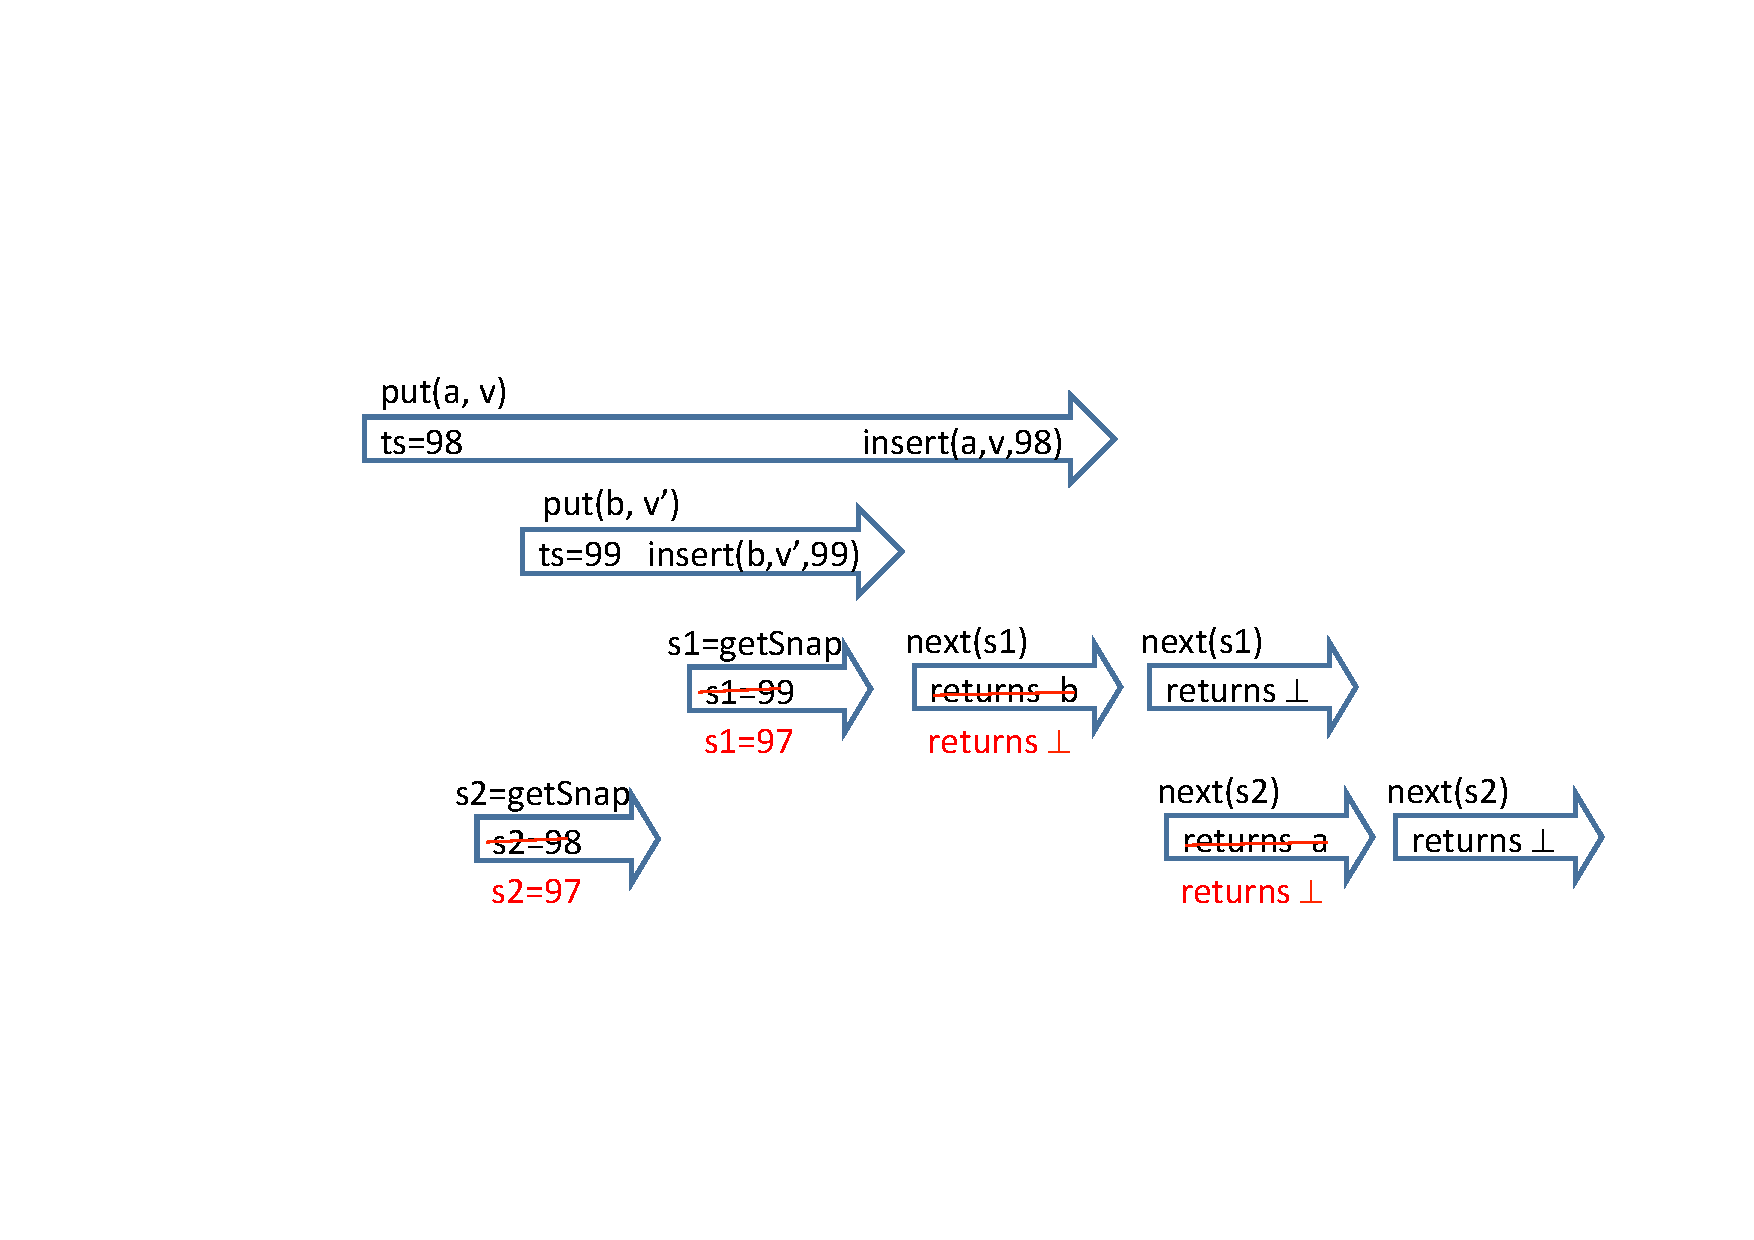
\includegraphics[width=\columnwidth, clip, trim=150 150 50
 		170]{Figures/scanExample}}

		\caption{Snapshots $s_1$ and $s_2$ cannot use the current
		values of \emph{timeCounter}, $99$ and $98$ respectively, since a \scode{next}
		operation pertaining to snapshot $s_1$ may miss the concurrently written key
		$a$ with timestamp $98$, while a \scode{next}
		operation pertaining to snapshot $s_2$ filters out the key $b$ with timestamp $99$.
		The snapshot time should instead be $97$, which excludes the concurrently
		inserted keys.}
\label{fig:snap-ts}
\end{figure}

We remedy this problem by tracking timestamps that were obtained but
possibly not yet written. These are kept in a set data structure, \emph{Active}, which can
be implemented in a non-blocking manner. The \scode{getSnap}
operation chooses a timestamp that is earlier than all active ones.
In the above example, since both $98$ and $99$ are active at the time
$s_1$ and $s_2$ are invoked, they choose $97$ as their snapshot time.


Note that a race can be introduced between obtaining a timestamp and inserting
it into \emph{Active} as depicted in Figure~\ref{fig:race}. In this example, a
\scode{put} operation reads timestamp $98$ from \emph{timeCounter}, and before
it updates the \emph{Active} set to include it, a
\scode{getSnap} operation reads timestamp $98$ from \emph{timeCounter} and finds
the \emph{Active} set empty. The snapshot timestamp is therefore set to $98$.
The value later written by the \scode{put} operation is not filtered out by
the scan, which may lead to inconsistencies, as in the previous example.
%
To overcome this race, the \scode{put} operation verifies that its chosen timestamp exceeds the latest snapshot's timestamp
(tracked in the \emph{snapTime} variable), and re-starts if it does not,
\eurosys{}{while \scode{getSnap} waits until all active \scode{put} operations
have timestamps greater than
\emph{snapTime}.%~\ref{code:snap:blocking}.
}

\begin{figure}[t]
\center
		{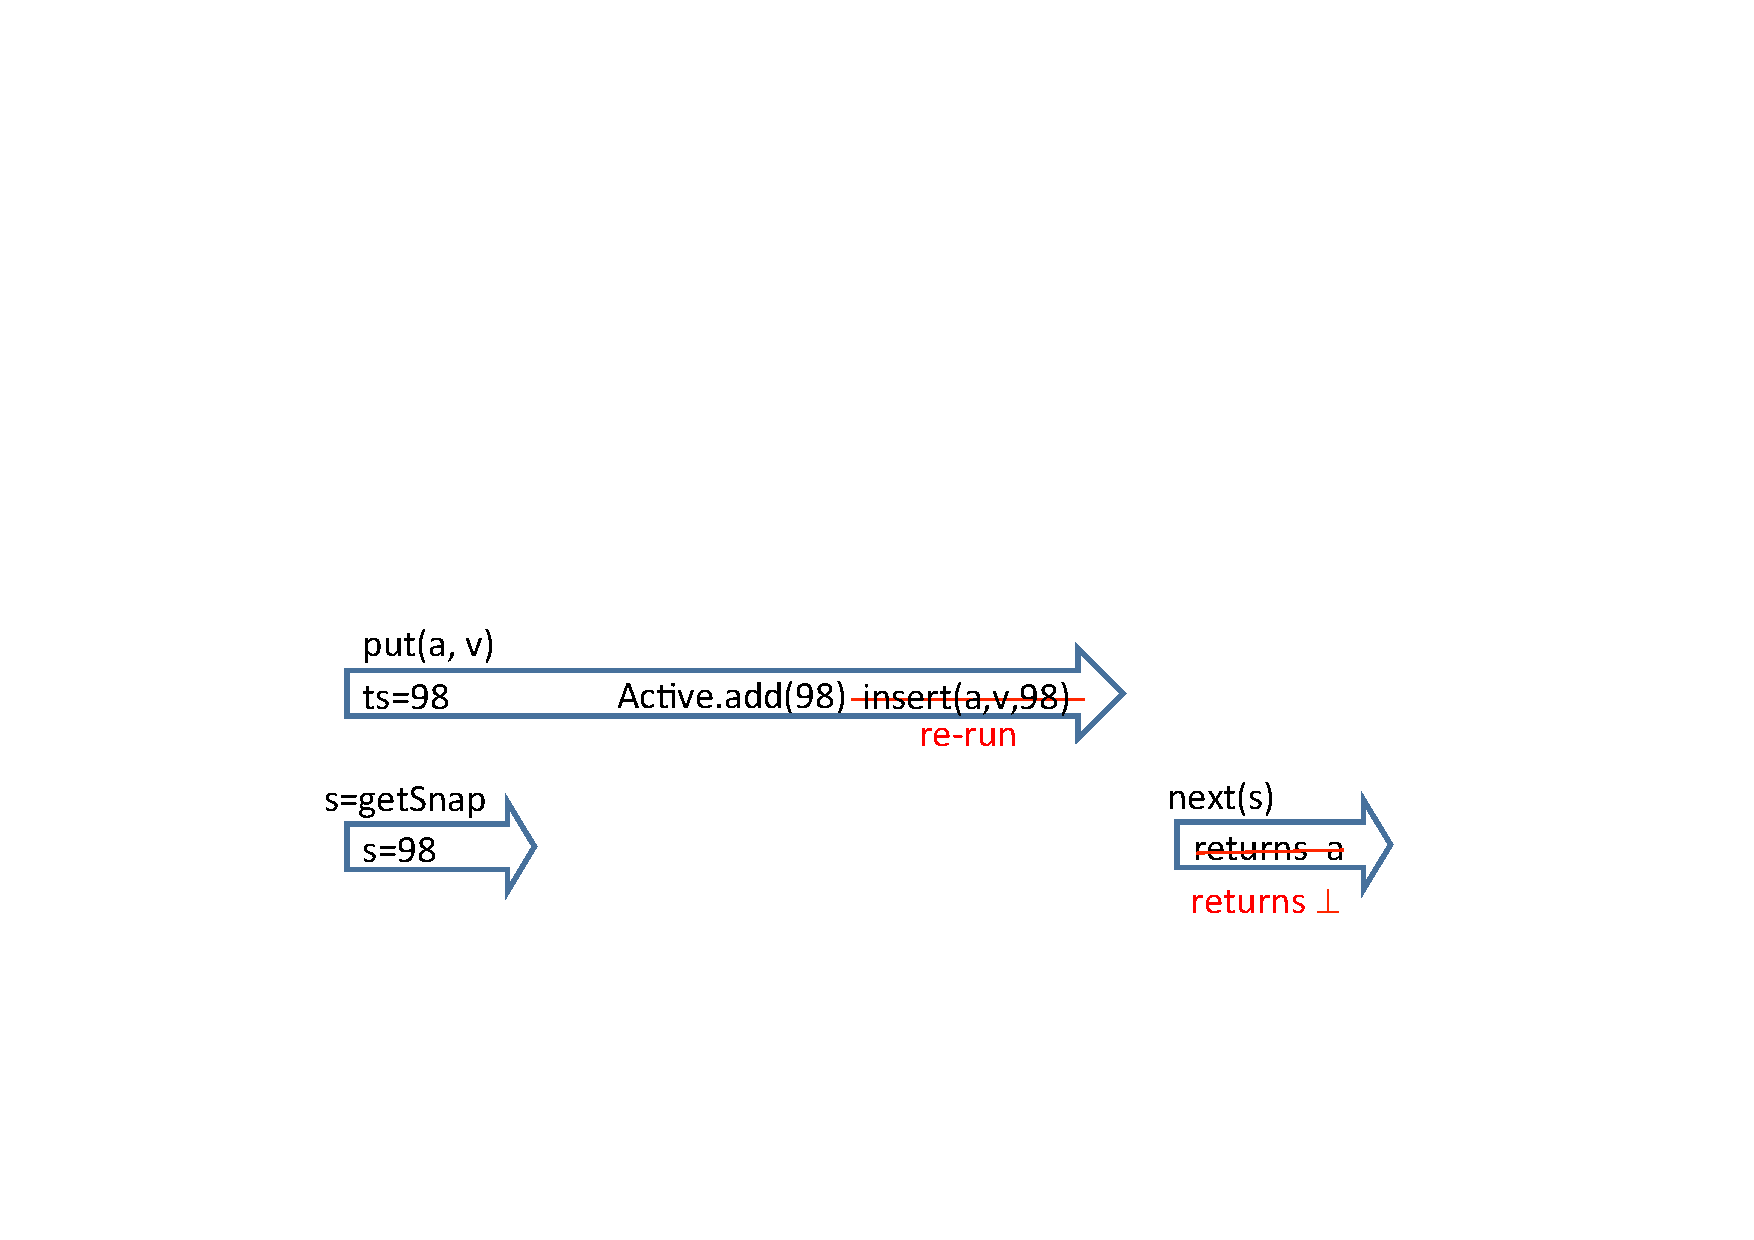
\includegraphics[width=\columnwidth, clip, trim=100 150 100
		300]{Figures/example3}}

		\caption{The put operation cannot use the value $98$ since a
		snapshot operation already assumes there are no active put operations
		before timestamp $99$. Using the timestamp $98$ may lead to the problem
		depicted in Figure~\ref{fig:snap-ts}. The put operation should instead
		acquire a new timestamp.}
  \label{fig:race}
\end{figure}

We note that our scan is serializable but not linearizable~\cite{Herlihy:1990}, in the sense that it can read a consistent state ``in the past''.
That is, it may miss some recent updates,
(including ones written by the thread executing the scan). To preserve
%the \emph{per-thread order}
linearizability, the \scode{getSnap} operation could be modified to wait until it is able
to acquire a \emph{snapTime} value greater than the  \emph{timeCounter}
value at the time the operation started. 
\eurosys{}{This can be done by omitting
lines~\ref{code:active:ts}-\ref{code:snap:ts} in
\algref{snapAlg}. }
%However, in cases where a thread is not
%required to scan its own updates this blocking implementation is not necessary.

Since puts are implemented as insertions with a new timestamp, the key-value store potentially holds many versions for a given key.
Following standard practice in LSM-DS,
old versions are not removed from the memory component, i.e., they exist at least until the component is discarded following its merge into disk.
Obsolete versions are removed during a merge once they are no longer needed for any snapshot.
In other words, for every key and every snapshot, the latest version of the key
that does not exceed the snapshot's timestamp is kept. % in some component.
%We assume an API for installing and removing snapshots which allows reclamation
%of associated values by the merge.

To consolidate with the merge operation, \scode{getSnap} installs the snapshot
handle in a  list  that captures all active snapshots.
Ensuing merge operations query the list to identify the maximal
timestamp before which versions can be removed. To avoid a race between installing a snapshot
handle and it being observed by a merge, the data structure is accessed while
holding the lock. The \scode{getSnap} operation acquires the lock in
shared mode while updating the list, and \scode{beforeMerge} queries the list while holding the
lock in exclusive mode. The timestamp returned by
\scode{beforeMerge} is then used by the merge operation to determine which
elements can be discarded. 
\eurosys{I3}{
%We assume there is a function that removes snapshots by
%removing their handles from the list, either per a user's request, or based on
% TTL.
As in levelDB, we assume handles of unused snapshots are removed
from the list either by the application (through an API call), or based on TTL;
failing to do so may reduce the amount of available memory for useful data.}
%an API for removing the snapshot handle
%from the list when the snapshot is discarded (omitted from the pseudocode).

\begin{algorithm} [t]
\small
\caption{\small  \clsm\ snapshot algorithm.}
\label{alg:snap}
%
\begin{algorithmic}[1]
\makeatletter\setcounter{ALG@line}{0}\makeatother
%
\Procedure{put}{Key $k$, Value $v$}
    \State \emph{Lock}.lockSharedMode()
		\State $ts \gets$ getTS()
    \State $P_{m}$.insert($k,ts,v$)
    \State \emph{Active}.remove($ts$)
    \State \emph{Lock}.unlock()
\EndProcedure
%
\vspace{3pt}
%
% \Procedure{get}{Key $k$}
% %	  \If {$s=\NULL$ } $s \gets \infty$ \EndIf
%     \State find $v$ s.t.\ $(k,ts,v)$ has
%     	highest $ts$ in $P_{m}$, $P'_{m}$, or $P_{d}$
%     \State return $v$
% \EndProcedure
% %
% \vspace{3pt}
% %
% \Procedure{next}{Snapshot $s$}
% %	\Repeat
%     \State $k \gets$ smallest key greater than \emph{current} in $P_{m}$,
%     $P'_{m}$, and $P_{d}$  %in $\{K\}$
%     \State \emph{current} $\gets k$
%     \State find $v$ s.t.\ $(k,ts,v)$ has
%     	highest $ts \leq$ $s$ in $P_{m}$, $P'_{m}$, or $P_{d}$
% %    \Until {$v$ is not marked as deleted}
%     \If {$v$ is marked as deleted} restart \EndIf
%     \State return $\langle k, v \rangle$
% \EndProcedure%
% \vspace{3pt}
%
\Procedure{getSnap}{}
    \State \emph{Lock}.lockSharedMode()
    \State $ts \gets$ \emph{timeCounter}.get()
    \State $ts_a \gets$ \emph{Active}.findMin() \label{code:active:ts}
    \If {$ts_a \not= \NULL$} $ts \gets ts_a - 1$ \EndIf \label{code:snap:ts}
    \State atomically assign $\max(ts, snapTime)$ to \emph{snapTime}  \label{LineSnapTime}
    \While{\emph{Active}.findMin() $<$ \emph{snapTime}} nop
    \label{code:snap:blocking} \EndWhile \State $ts_b \gets snapTime$
    \State install $ts_b$ in the active snapshot list
    \State \emph{Lock}.unlock()
    \State return $ts_b$
\EndProcedure
%
\vspace{3pt}
%
\Procedure{getTS}{}
		\While{\emph{true}}
			\State $ts \gets$ \emph{timeCounter}.incAndGet()
			\State \emph{Active}.add($ts$)
			\If {$ts \leq$ \emph{snapTime} } 	\emph{Active}.remove($ts$) \Else \emph{
			break} \EndIf
		\EndWhile
		\State return $ts$
\EndProcedure
\vspace{3pt}
%
\Procedure{beforeMerge}{}
   \State \emph{Lock}.lockExclusiveMode()
   \State $P_{m}^{'} \gets P_{m}$
   \State $P_{m} \gets$ new in-memory component
   \State $ts \gets$ find minimal active snapshot timestamp
   \State \emph{Lock}.unlock()
   \State return $ts$
\EndProcedure
%

\end{algorithmic}
\label{Al:snapAlg}
\end{algorithm}

\remove{
Our snapshot management algorithm appears in \algref{snapAlg}.
The \scode{put}
and \scode{getSnap} procedures select timestamps as explained above.
The  \scode{get} operation now returns the highsest timestamped value for the given key.
% The \scode{next} operation takes a snapshot as a parameter, and returns, for every key found by the components' iterators,
% the value associated with the highest timestamp smaller than the snapshot time.
Note that since $P_m$ always holds the latest inserted values, and $P_m^{'}$
holds values no older than those in $P_d$, \scode{get} may return as soon as it finds a value older than the requested snapshot
either in $P_m$ or in $P_m^{'}$.
}

Because more than one  \scode{getSnap} operation can be executed concurrently,
we have to update  \emph{snapTime}  with care, to ensure that it does not move backward in time.
We therefore atomically advance \emph{snapTime} to $ts$ 
(e.g., using a CAS\footnote{\emph{Compare and Swap} operation~\cite{Herlihy2008}.}) in line \ref{LineSnapTime}.
%
The rollback loop in \scode{getTS} may cause the starvation of a \scode{put}
operation. We note, however, that each repeated attempt to acquire a timestamp
implies the progress of some other \scode{put} and \scode{getSnap} operations, as expected in non-blocking
implementations.

\subsubsection{Partial Scans and Snapshot Reads}
\label{se:range}

A full snapshot scan traverses
all keys starting with the lowest and ending with the highest one. More common
are partial scans, (e.g., range queries),
in which the application only traverses a small consecutive range of the keys,
or even simple reads of a single key from the snapshot.
Given our snapshot management mechanism, it is straightforward to support these by using
a \eurosys{I5}{find function to locate the first entry to be retrieved (like
finding a key in a \scode{get} operation)}.

\subsection{Atomic Read-Modify-Write}
\label{Se:RMW}

We now introduce a general read-modify-write operation, \scode{RMW(k,f)}, which atomically applies an
arbitrary function $f$ to the current value $v$ associated with key $k$ and stores $f(v)$
in its place.
Such operations are  useful for many applications, ranging from simple vector clock update and validation to implementing full-scale transactions.

%Many state-of-the-art data store implementations  do not provide such general atomic read-modify-write operations. Nevertheless, such operations are extremely useful for many applications, ranging from simple vector clock update and validation to implementing full-scale transactions.

Our solution is efficient and avoids blocking. It is given in
the context of a specific implementation of the in-memory data store as a linked
list or any collection thereof, e.g., a skip-list. Each entry in the linked list
contains  a key-timestamp-value tuple, and the linked list is sorted in
lexicographical order. In a non-blocking implementation of such a data
structure, \scode{put} updates the \emph{next} pointer of the
predecessor of the inserted node using a CAS operation~\cite{Herlihy2008}.

The pseudo-code for read-modify-write on an in-memory linked-list appears in
\algref{RMWAlg}.
The  idea is to use optimistic concurrency control -- having read $v$ as the latest
value of key $k$, our attempt to insert $f(v)$ fails (and restarts) in case a new value has been inserted for $k$ after $v$.
This situation is called a \emph{conflict},
and it means that some concurrent operation has interfered between our read step in line~\ref{LineReadTuple} and our update step in  line~\ref{CASLine}.

\begin{algorithm} [t]
\small
\caption{\small RMW algorithm for linked list memory component.}
\label{alg:RMW}
%
\begin{algorithmic}[1]
\makeatletter\setcounter{ALG@line}{0}\makeatother
%
\Procedure{RMW}{Key $k$, Function $f$}
    \State \emph{Lock}.lockSharedMode()
		\Repeat
	    \State find $(k,ts,v)$ with highest $ts$ in  $P_{m}$, $P'_{m}$, or $P_{d}$ \label{LineReadTuple}
  	  \State \emph{prev} $\gets$ $P_{m}$ node with $\max (k',ts') \leq (k,\infty)$ \label{LineSetPrev}
      \If {\emph{prev.key} $= k$ and \emph{prev.time} $> ts$} continue  \label{conflict1Line}   \EndIf \Comment{conflict}
  	  \State \emph{succ} $\gets$ \emph{prev.next} \label{LineSetNext}
  	  \If {\emph{succ.key} $= k$} continue  \label{conflict2Line}  \Comment{conflict} \EndIf
	  	\State $ts_n \gets$ getTS() \label{newTS}
    	\State create \emph{newNode} with $(k,ts_n,f(v))$
    	\State \emph{newNode.next} $\gets$ \emph{succ}
	    \State \emph{ok} $\gets$ CAS(\emph{prev.next, succ, newNode}) \label{CASLine}
      \If { $\neg$\emph{ok} } \emph{Active}.remove($ts_n$) \Comment{conflict}
      \EndIf
    \Until { \emph{ok} }	
    \State \emph{Active}.remove($ts_n$)
    \State \emph{Lock}.unlock()
\EndProcedure
%
\end{algorithmic}
\label{Al:RMWAlg}
\end{algorithm}

The challenge is to detect conflicts efficiently.
Here, we take advantage of the fact that all updates occur in RAM, ensuring that all conflicts will be manifested in the in-memory component.
We further exploit the linked list structure of this component.
In line~\ref{LineSetPrev}, we locate, and store in \emph{prev}, the insertion point for the new node.
%
If \emph{prev} is a node holding key $k$ and a timestamp higher than $ts$,
then it means that another thread has inserted a new node for $k$ between lines~\ref{LineReadTuple} and \ref{LineSetPrev} ---
this conflict is detected in line~\ref{conflict1Line}.
%
In line~\ref{conflict2Line}, we detect a conflict that occurs when
another thread inserts a new node for $k$ between lines~\ref{LineSetPrev} and
\ref{LineSetNext} --- this conflict is observed when \emph{succ} is a node
holding key $k$.
%
If the conflict occurs after line~\ref{LineSetNext}, it is detected by failure of the CAS in line~\ref{CASLine}.

%In case $k$ was already in the in-memory list, \emph{prev} is a node holding key $k$, and otherwise, it holds a smaller key.
%A conflict is reflected by a change to the successor of \emph{prev}.
%If it changes before we read it into \emph{succ} in line~\ref{LineSetNext}, we detect the conflict in line~\ref{conflictLine}.
%If the conflict occurs after line~\ref{LineSetNext}, the conflict is detected by failure of the CAS in line~\ref{CASLine}.


\remove{
For example, consider a \scode{RMW} operation on key $15$, and assume that this key is found in
the disk component.
When the operation begins, \emph{prev} is set to some node $n$ holding the largest key smaller than $15$.
Assume now that a concurrent \scode{put} operation inserts a new value for key $15$. This value is
also inserted after $n$.
If  \scode{put}  changes \emph{n.next}  before line~\ref{LineSetNext}, then
the conflict is detected in line~\ref{conflictLine}. If it changes
after the \scode{RMW} operation executes line~\ref{LineSetNext} and before it executes line~\ref{CASLine},
then the CAS fails, and again, the operation restarts.
Otherwise, the \scode{put} operation is ordered after the \scode{RMW}, and there is no conflict.
}

When the data store consists of multiple linked lists, as
\emph{libcds}'s lock-free skip-list does~\cite{libcds}, items are inserted to
the lists one at a time, from the bottom up~\cite{Herlihy2008}.
Only the bottom  list is required for correctness, while the others ensure the
logarithmic search complexity. Our implementation thus
% , like \emph{libcds}'s lock-free skip-list~\cite{libcds},
first inserts the new item
to the bottom list atomically using \algref{RMWAlg}. It then adds the item to each higher list using a CAS as
in line~\ref{CASLine}, but with no need for a new timestamp~\ref{newTS} or
conflict detection as in lines~\ref{conflict1Line} and~\ref{conflict2Line}.

We note that the lock-free skip-list \cite{libcds}
 (which is based on the skip-list algorithm in~\cite{Herlihy2008})
satisfies the requirements specified in Section~\ref{Se:Snapshots} ---
%Although, in the general case, this data structure does not  guarantee weak
% consistency, in our case it does ensure this property.
%In this data structure,
weak consistency is guaranteed as long as items are not
removed from the skip-list, as is the case in \clsm.
% --- and in our algorithm, items are never removed from the skip-list as long as it is being used.
%(Items are removed and freed only when the entire skip-list is freed).





\section{Implementation}
\label{sec:impl}

We implement \clsm\ in C++ based on the popular open source {\leveldb} LSM-DS library~\cite{leveldb}.
{\leveldb} is used by numerous applications including Google Chrome and
Facebook's embeddable  key-value store~\cite{RocksDB}.
%Facebook's distributed key-value store back-end (RocksDB~\cite{RocksDB}).

{\leveldb\/} implements a rich API that includes read (get), write (put), and various snapshot operations.
Its memory component is implemented as a skip list with custom concurrency control.
%{\leveldb\/} is durable -- i.e.,
Every write is logged to a sequential
file following the LSM-DS update. Typically, the data store is configured to perform logging asynchronously,
which allows writes to occur at memory speed; hence, a write only queues the request for logging and a handful of writes may be lost due to a crash.
{\leveldb\/} features a number of optimizations, including multilevel merge, custom memory allocation,
caching via memory-mapped I/O,  Bloom filters~\cite{Bloom1970} to speed up reads, etc.

The original {\leveldb\/} acquires a global exclusive lock to protect critical sections at the beginning
and the end of each read and write. The bulk of the code is guarded by a mechanism
that allows a single writer thread and multiple reader threads to execute at any given time.
Snapshots are implemented using timestamps -- the timestamp management is simpler than ours (i.e., no  need for \emph{Active} set) since concurrent write operations are not permitted.
{\leveldb\/} supports an atomic batch of write operations that is implemented using coarse-grained synchronization of simple write operations.
%\Idit{Please say how snapshots are implemented-- does it use a \emph{timeCounter} like we do?
%Does it use a lock to avoid the need for \emph{Active}? What about atomic batch operations?}

{\clsm\/} supports the full functionality of {\leveldb}'s API.
Its implementation inherits the core of {\leveldb}'s modules (disk component, cache, merge function, etc), and benefits
from the same optimizations.
It implements the algorithm described in Section~\ref{sec:algorithm}, which eliminates the blocking parts of the
{\leveldb\/} code.
Our support for atomic batches of write operations continues to block (similarly to the original {\leveldb\/}) --
its synchronization is implemented by holding the shared-exclusive lock in exclusive mode.

We harness the \emph{libcds} concurrent data structures' library~\cite{libcds}
to implement the in-memory store and the logging queue (via the non-blocking skip list and queue implementations, respectively).
We also implement multiple custom tools based
on atomic hardware instructions: a shared-exclusive lock, and a non-blocking memory allocator~\cite{michael2004scalable}.
%, and non-blocking timestamp and reference counters.
\eurosys{I6}{All accesses we add to shared memory are protected by memory
fences, whereas the libraries we use include fences where deemed necessary by their developers.}

%The RMW abstraction is not supported by {\leveldb\/} originally. {\clsm\/} implements its popular put-if-absent
%variation~\cite{Herlihy2008}, based on our algorithm. To establish a comparison baseline, we augment {\leveldb\/}
%with a textbook \emph{lock-striping} implementation~\cite{GrayTP1993} (Section~\ref{sec:eval}).

Relaxing {\leveldb}'s single-writer constraint implies that writes might get logged out of order.
Since all the log records bear {\clsm}-generated timestamps, the correct order is easily
restored upon recovery.

%The RMW abstraction is not supported by {\leveldb\/} originally.
%To establish a comparison baseline, we augment {\leveldb\/}
%with a textbook \emph{lock-striping} implementation~\cite{GrayTP1993} (Section~\ref{sec:eval}).

\section{Evaluation}
\label{sec:eval}


We evaluate our {\clsm\/} implementation versus a number of open source competitors.
%, in terms of throughput and latency, on a suite of benchmarks.
In Section~\ref{sec:microbenchmarks}, our experiments are based on  synthetic CPU-bound workloads.
In Section~\ref{sec:realworkloads} we use real web-scale application workloads.
Finally, in Section~\ref{sec:heavyCompaction}, we use a synthetic disk-bound benchmark from {\rocksdb}'s benchmarks suite~\cite{RocksDBBenchmarks}.

%Our experiments include synthetic benchmarks as well as real web-scale
%application workloads. They exercise different combinations of reads, writes, read-modify-writes,
%and snapshot scans in CPU-bound scenarios.

Our platform is a Xeon E5620 machine with 2 quad-core CPUs, each core with
two hardware threads (16 hardware threads overall).
The server has 48GB of RAM and 720GB SSD storage\footnote{Composed of four 240GB SSD SATA/300 OCZ Deneva MLC, configured as RAID-5.}.

We vary the concurrency degree in our experiments from one to sixteen worker threads performing operations;
these are run in addition to the maintenance compaction thread (or threads in Section~\ref{sec:heavyCompaction}).


We compare {\clsm} with four open-source LSM data stores: {\leveldb}~\cite{leveldb},
{\hyperleveldb}~\cite{Hyperdex2012,HyperLevelDB}, {\rocksdb}~\cite{RocksDB}, and {\blsm}~\cite{BLSM2012}.
{\hyperleveldb} and {\rocksdb} are extensions of  {\leveldb} that employ specialized  synchronization to improve parallelism
(see~\cite{RocksDBOptimizedLocks}),
and {\blsm\/} is a single-writer prototype that capitalizes on careful scheduling
of merges.
%
Unless stated otherwise, each LSM store is configured to employ an in-memory
component of 128MB \eurosys{E2}{(this is the standard value in key-value stores
like HBase)}; we use the default values of all other configurable parameters.

Recall that in LSM-DS, component merges occur as a background process, which is often called \emph{compaction}.
All systems except {\rocksdb} use a single background thread for compaction.
{\rocksdb} has a configurable parameter determining the maximum number of compaction threads,
which we set to one\footnote{This is the default value in {\rocksdb}.}, except in Section~\ref{sec:heavyCompaction}.
We note that in experiments that involve writes (i.e., put operations), the compaction thread is working a significant  portion of the time --- in the CPU-bound experiments reported in Sections~\ref{sec:microbenchmarks} and~\ref{sec:realworkloads}, we found that it runs  roughly between a quarter and three-quarters of the time, in all systems. In Section~\ref{sec:heavyCompaction} we consider disk-bound workloads, where compaction runs virtually all the time, and creates a bottleneck.

\subsection{Synthetic Workloads}
\label{sec:microbenchmarks}


We start with a set of benchmarks that exercise the systems in a variety of controlled settings.
%The benchmarks experiment with concurrency degrees from 1 to 16 threads.
Our experiment harnesses a 150GB dataset (100x the size of the
collection used to compare {\hyperleveldb\/} to {\leveldb\/} in the publicly available
benchmark~\cite{hyperdex}).
The key-value pairs have 8-byte keys, and the value size is $256$ bytes.


 {\bf {Write performance.}}
We start by exploring a write-only workload.
The keys are drawn uniformly at random from the entire range.
(Different distributions lead to similar results --
recall that the write performance in LSM stores is locality-insensitive.)

Figure~\ref{fig:100w_throughput} depicts the results in terms of throughput.
{\leveldb}, {\hyperleveldb\/}, and {\clsm\/} start from approximately the same point, but
they behave differently as we increase the number of threads.
{\leveldb}, {\blsm} and {\rocksdb} are bounded by their single-writer
architectures, and do not scale at all. \eurosys{E5}{Moreover, having multiple
threads contending for a single synchronization point (e.g., a writers queue)
causes the throughput to decrease.} {\hyperleveldb} achieves a $33\%$ throughput
gain with $4$ workers, and deteriorates beyond that point.
{\clsm\/}'s throughput scales $2.5$x and becomes saturated at $8$ threads. \eurosys{E4}{The degragation in write performance can be explained by cross-chip latency and cache invalidations, since only the 16 threads experiment spans more than one chip.} {\clsm\/}'s peak rate
exceeds $430$K writes/sec, in contrast with $240$K for {\hyperleveldb}, $160$K for {\leveldb} and $65$K for {\rocksdb}.
%
%Note that {\clsm\/}'s peak performance is achieved with $8$ threads. This happens due to
%intensive cache synchronization between the two CPU's, as all cores perform frequent atomic
%hardware instructions.


%\clsm's advantage can be explained via its improved CPU utilization. For example, with 8 threads {\clsm}'s per-core
%sustained utilization reaches 94\%, whereas {\leveldb}'s is just above 40\%.


Figure~\ref{fig:100w_latencyVSthroughput} refines the results by
presenting the throughput-latency perspective, where the latency is computed
for the $90$-th percentile; other percentiles exhibit similar trends.
For better readability we delineate improvement trends and omit points
exhibiting decreasing throughput. This figure marks the point in which
each implementation saturates, namely, either achieves a slight
throughput gain while increasing the latency by a factor of $2$x-$3$x or
achieves no gain at all. \eurosys{E}{It is clear that {\clsm} scales better than all competitors.}

%Figure~\ref{fig:100w_latency} compares the systems in terms of latency (the median,
%the 90\% and the 99\%), for $8$ threads.
%{\clsm} achieves the lowest latency, e.g., with
%8 threads its median write latency is 15 {\microsec}, and the 90th percentile is
%31 {\microsec}. The single-writer implementations are most vulnerable to latency
%variability -- e.g., for {\leveldb\/} and {\blsm\/} the median latencies exceed
%75 {\microsec} and 100 {\microsec}, respectively.

%{\color{red}
%Our measurements show that scans support in {\clsm}'s writes (active set
%maintenance, see Section~\ref{sec:algorithm}) incurs insignificant overhead in
%most cases.
%For applications that do not require snapshot scans, stripping the
%snapshot-support code can boost throughput in some settings up to 15\% beyond
%the demonstrated numbers.
%}



\begin{figure*}%[t]
  \centering
  \begin{subfigure}[t]{0.49\textwidth}
   \center
   \fbox{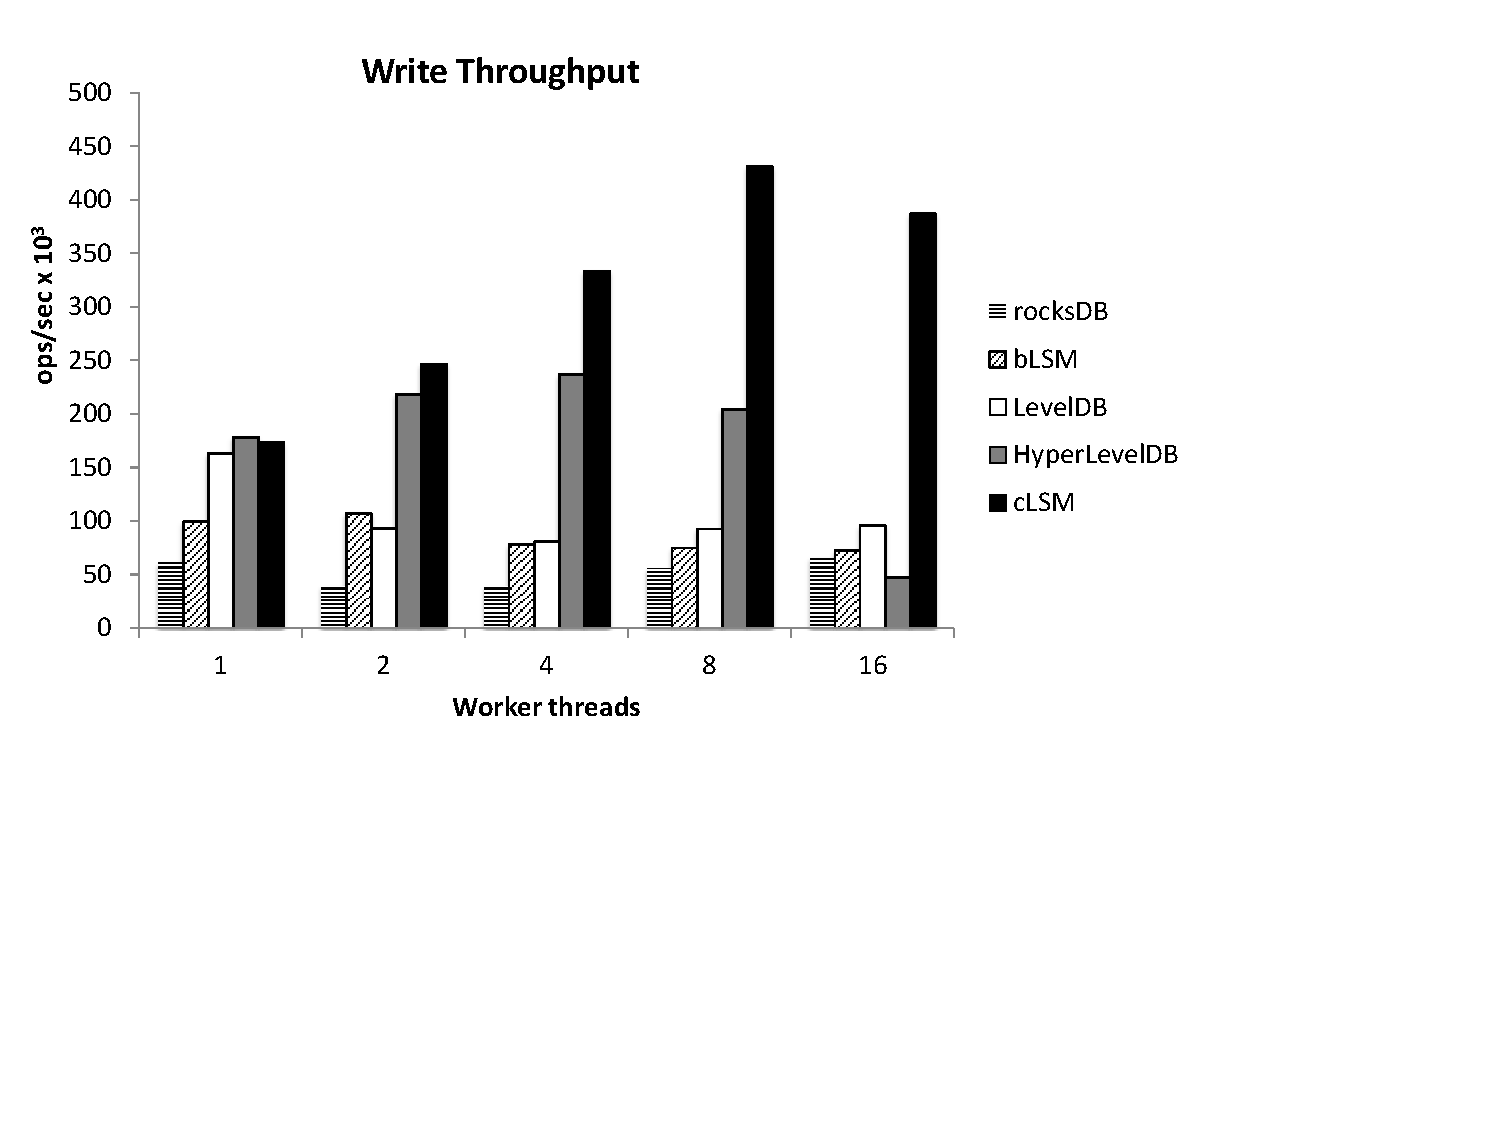
\includegraphics[width=0.9\textwidth,clip, trim =0 180 150 0]{Figures/100_write_throughput.pdf}}
		%{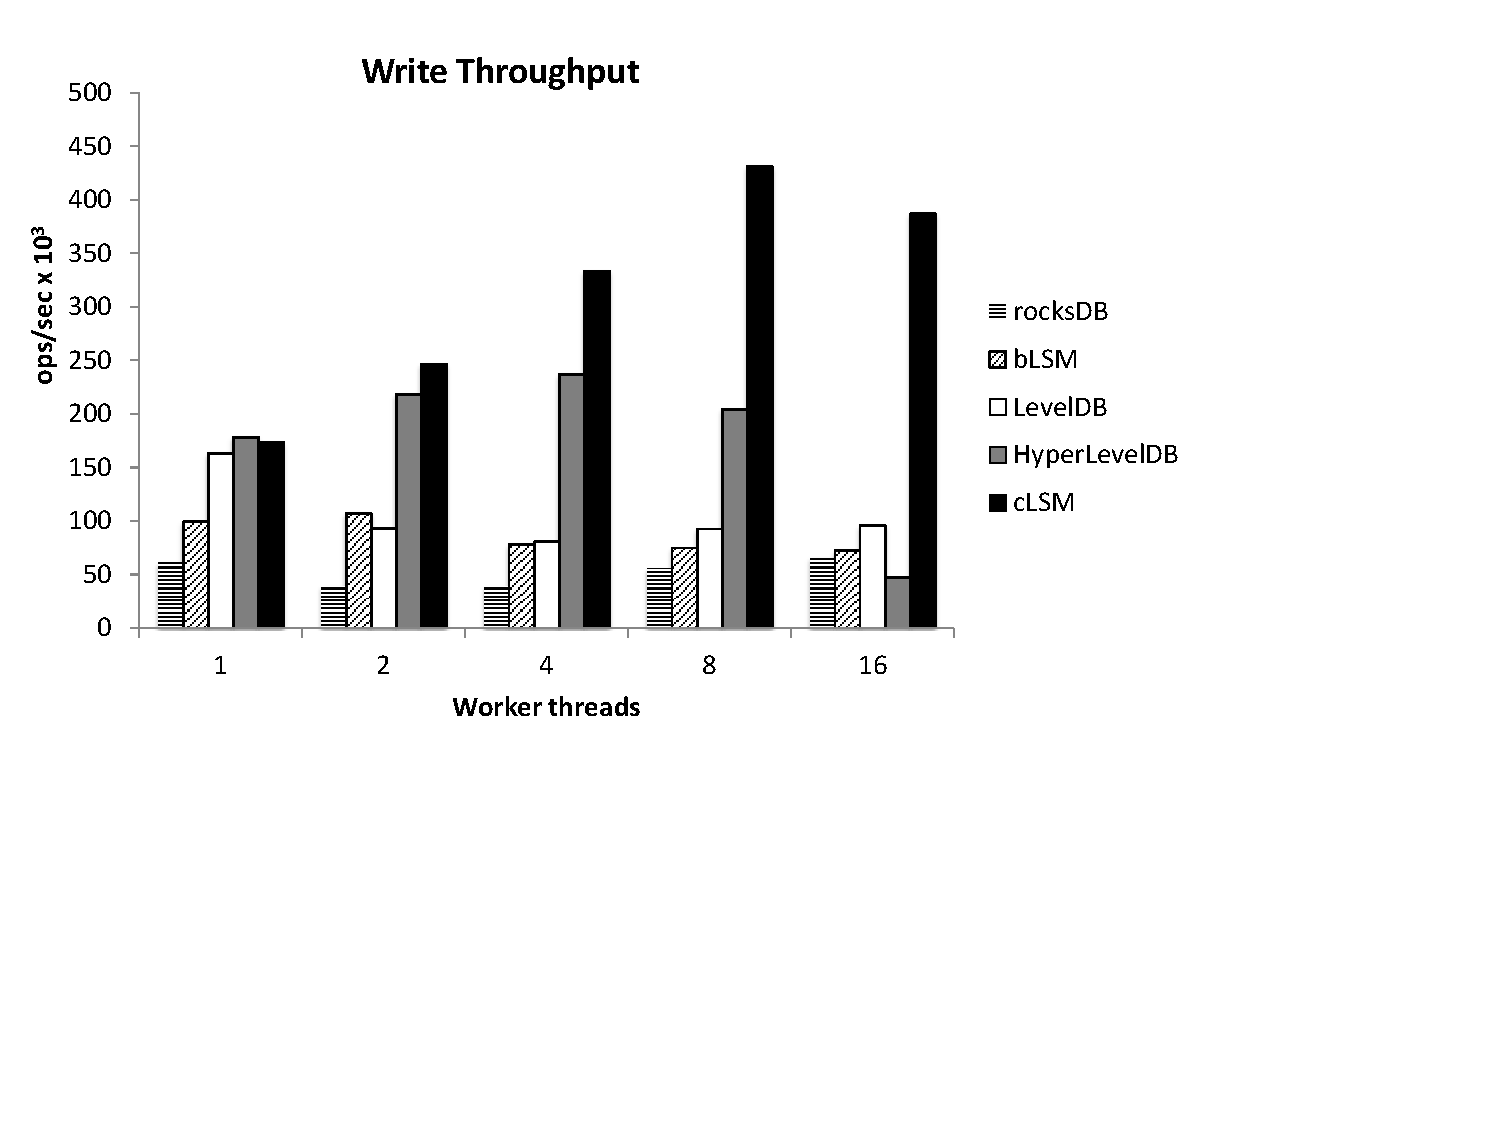
\includegraphics[height=1.8in]{Figures/100_write_throughput.pdf}}
		\caption{Throughput}
               \label{fig:100w_throughput}
  \end{subfigure}%
 %\hspace{0.2\textwidth}
  \begin{subfigure}[t]{0.49\textwidth}
   \center
		\fbox{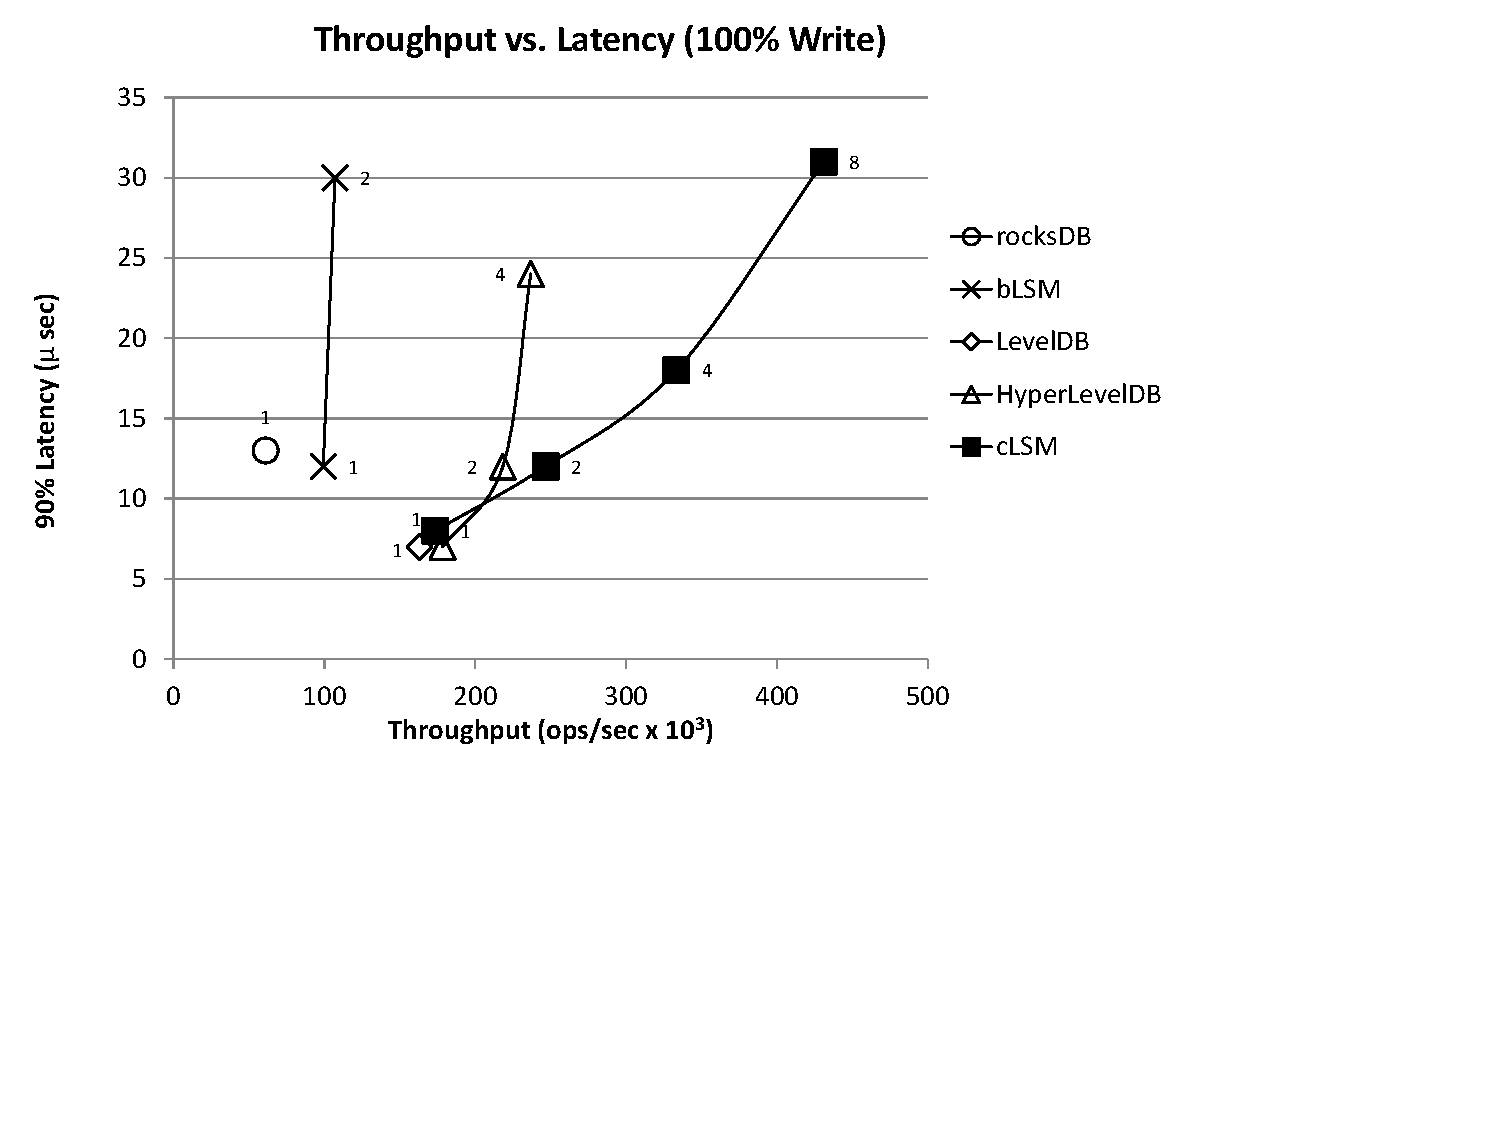
\includegraphics[width=0.9\textwidth,clip, trim =0 180 160 0]{Figures/100_write_latency_vs_throughput.pdf}}
		\caption{Throughput versus latency; each data point is labeled with the number of threads}
               \label{fig:100w_latencyVSthroughput}
  \end{subfigure}%
\caption{\bf{Write performance -- a 100\% write scenario, with the keys uniformly distributed across the domain.
{\clsm\/} scales to 8 threads and achieves 80\% throughput advantage over the closest competitor, which only scales to 4.
%With 8 threads -- {\clsm\/} is significantly faster in all latency percentiles.
}}
\label{fig:100w}
\end{figure*}





{\bf{Read performance.}}
We turn to evaluate performance in a read-only scenario. In this context,
uniformly distributed reads would not be indicative, since the system would spend most of the time in disk seeks,
devoiding the concurrency control optimizations of any meaning. Hence, we employ a skewed distribution that
generates a CPU-intensive workload: $90\%$ of the keys are selected randomly from ``popular'' blocks that
comprise $10\%$ of the database. The rest are drawn u.a.r. from the whole range. This workload is both dispersed
and amenable to caching. Its locality is similar to that of production workloads analyzed in
Section~\ref{sec:realworkloads}. All the following experiments exercise this distribution.


Figure~\ref{fig:100r_throughput} demonstrates throughput scalability.
{\leveldb\/} and  {\hyperleveldb\/} exhibit similar performance.
Neither scales beyond $8$ threads, reflecting the limitations of {\leveldb}'s concurrency control, \eurosys{E4}{namely, read operations blocking even when data is available in memory.}
On the other hand, {\clsm} and {\rocksdb} scale all the way to $128$ threads, far beyond
the hardware parallelism
(more threads than cores are utilized, since some threads block when reading data from disk).
In all cases, {\rocksdb} is not only slower than \eurosys{E}{{\clsm}, but even slower than {\leveldb\/}}.
%{\blsm} has similar performance in all cases.
In this experiment, the peak throughput of {\clsm} is almost $1.8$ million
reads/sec -- $2.3$x as much as the peak competitor rate.


%On the other hand, in {\clsm} the reads perform much fewer synchronization instructions, hence less CPU cache
%synchronization overhead is incurred. We see that {\clsm}  scales all the way to $128$ threads, far beyond
%the hardware parallelism.
%With this many threads, there are enough workers to saturate all available cores at any given moment.
%%(i.e., no throughput is wasted on threads blocked on cache misses).
%The peak throughput is almost $1.8$ million reads/sec -- 2.3x as much as the peak competitor rate.


Again, Figure~\ref{fig:100r_latencyVSthroughput} shows the throughput-latency (90-th percentile) perspective. This figure
emphasizes the scalability advantage of {\clsm}: it shows
that while {\rocksdb} scales all the way, this comes at a very high latency
cost, an order of magnitude higher than other {\leveldb}-based solutions with
the same throughput ($800$K reads/sec).

%%The read latencies depend on the system's internal parallelism.
%Figure~\ref{fig:100r_latency} depicts the latency
%distribution with 16 threads (when no thread is starved of a CPU resource). Here, {\clsm\/} exhibits a median latency
%of just 13 {\microsec}, and the 90\% latency is 17 {\microsec}. {\leveldb}'s and {\hyperleveldb}'s
%medians are 41 {\microsec} and 55 {\microsec}, respectively. The 99\% latencies are not shown since they are similar among all the
%data stores; these reads hit the disk, and hence, are two orders of magnitude slower.

\begin{figure*}
  \centering
  \begin{subfigure}[t]{0.49\textwidth}
   \center
		\fbox{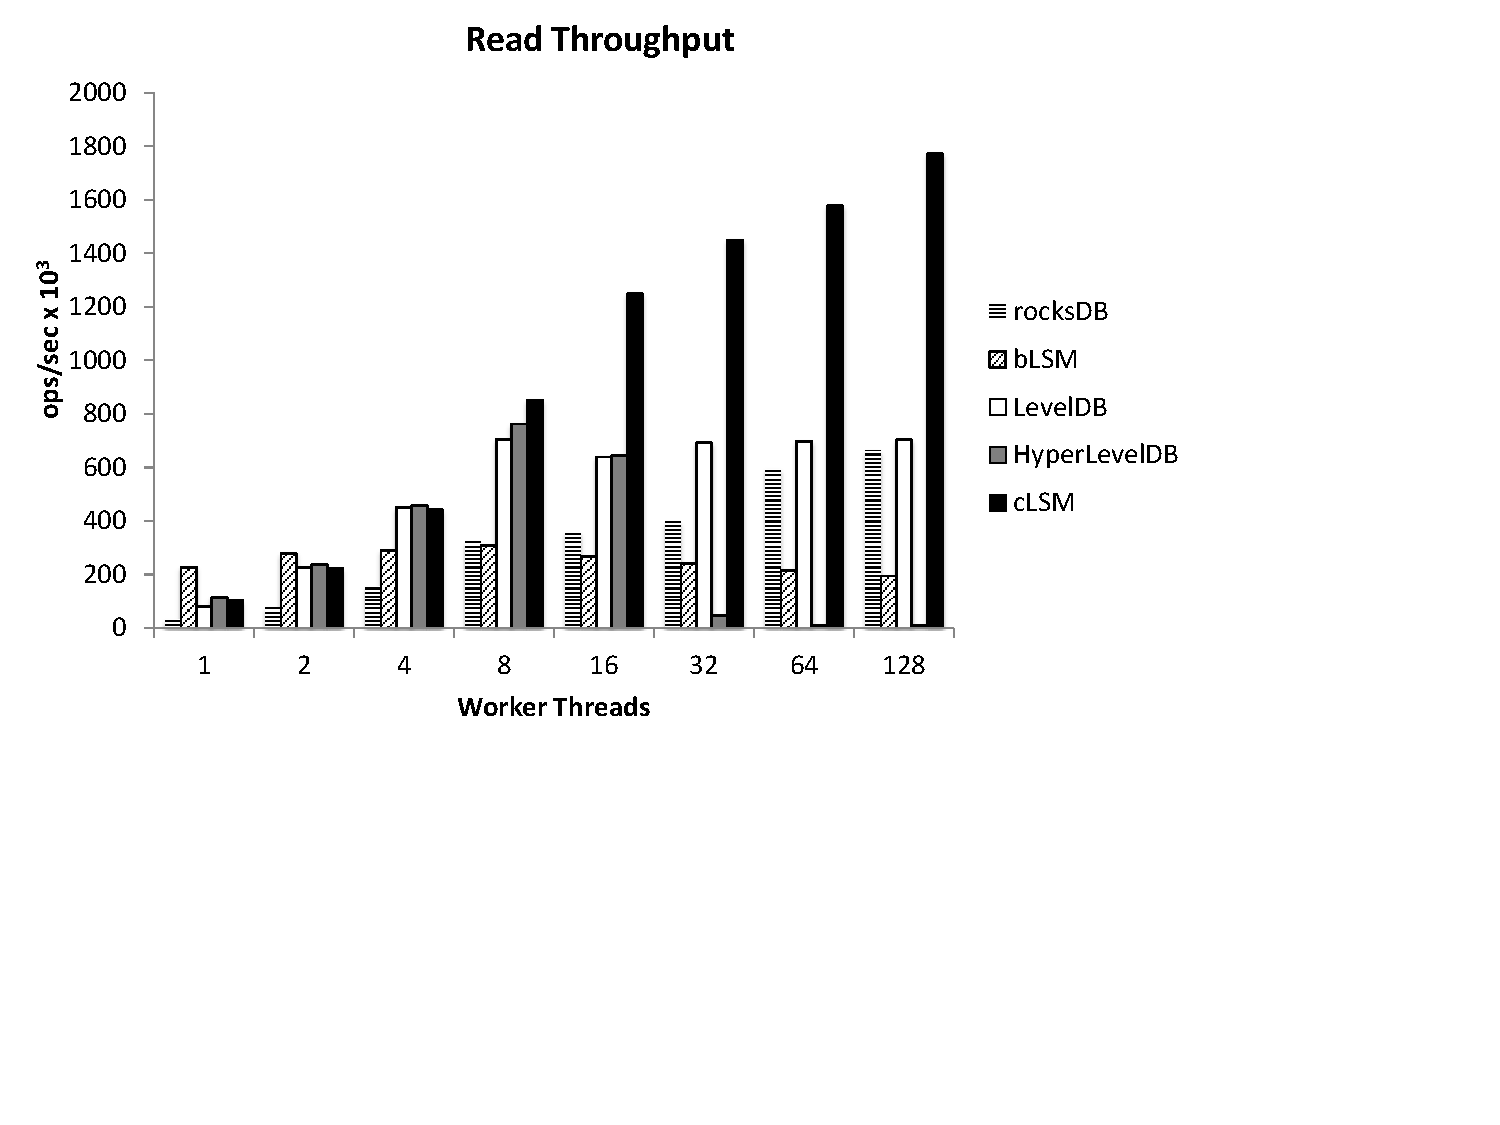
\includegraphics[width=0.9\textwidth,clip, trim =0 180 150 0]{Figures/100_read_throughput.pdf}}
		\caption{Throughput}
               \label{fig:100r_throughput}
  \end{subfigure}%
%\quad
% \hspace{0.2\textwidth}
  \begin{subfigure}[t]{0.49\textwidth}
   \center
        \fbox{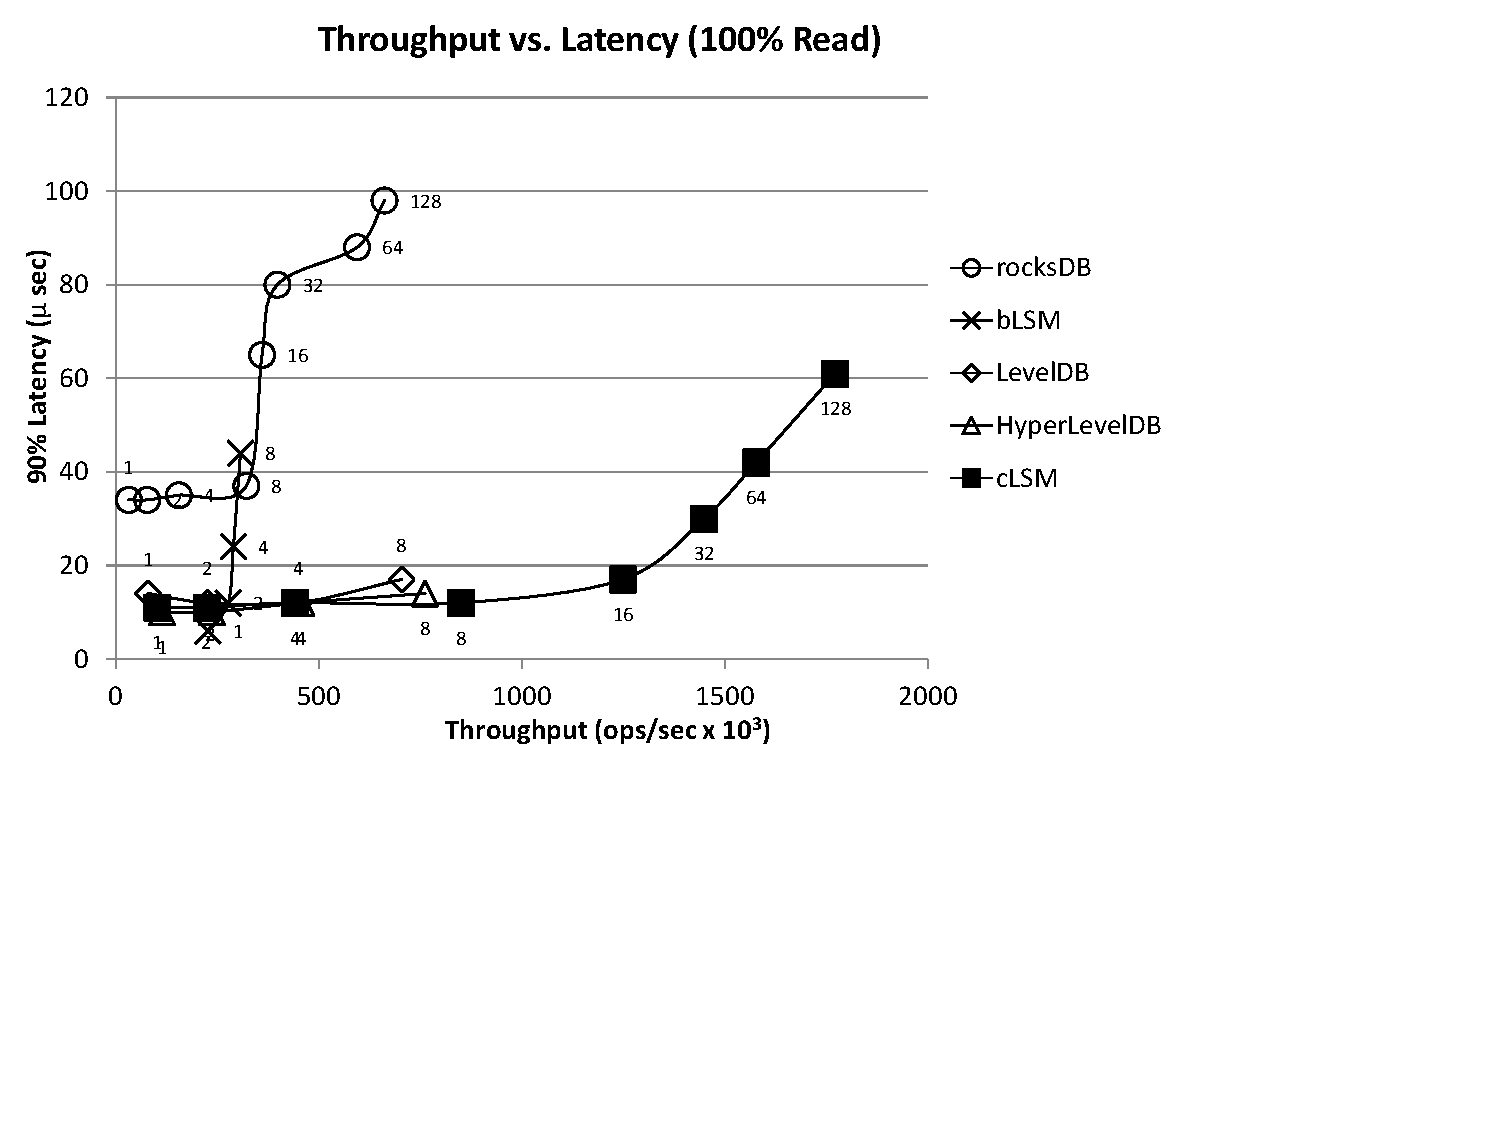
\includegraphics[width=0.9\textwidth,clip, trim =0 180 160 0]{Figures/100_read_latency_vs_throughput.pdf}}
		%{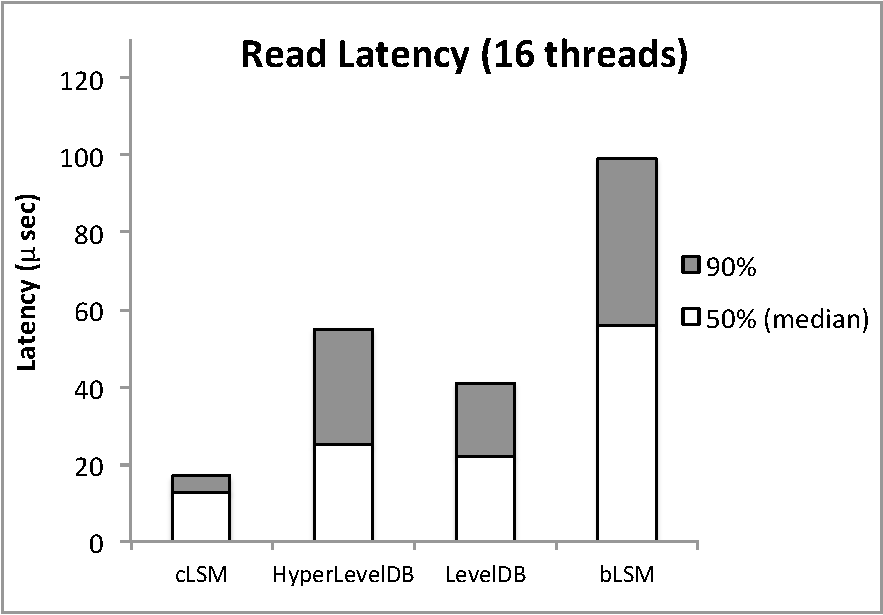
\includegraphics[height=1.8in]{Figures/100_read_16_thread_latency.pdf}}
		\caption{Throughput versus latency; each data point is labeled with the number of threads}
               \label{fig:100r_latencyVSthroughput}
  \end{subfigure}%
\caption{\bf{Read performance -- a 100\% read scenario with locality (90\% of keys picked from 10\% popular blocks).
%{\clsm\/} scales to 128 threads and achieves 130\% throughput advantage over the closest competitor.
}}
\label{fig:100r}
\end{figure*}




{\bf {Mixed workloads.}}
Figure~\ref{fig:50r50w_throughput} depicts the throughput achieved by the different systems
under a 1:1 read-write mix. %The results are consistent with the previous sections.
The original {\leveldb\/} fails to scale, even though the writes are now
only 50\% of the workload.
{\hyperleveldb\/} slightly improves upon that result, whereas {\clsm\/} fully
exploits the software parallelism, scaling beyond 730K operations/sec with 16 workers.

\eurosys{E4}{We note that while under {\clsm\/} and {\hyperleveldb\/} the reads and the writes scale independently (and the throughput numbers are roughly the avarage of the 100\% writes  and 100\% reads scenarios), in  {\leveldb\/} and  {\rocksdb} the writes impede the reads' progress, and therefore the absolute numbers are lower than the average of the 100\% writes  and 100\% reads scenarios.}


Figure~\ref{fig:50scan50w_throughput} repeats the same experiment with reads replaced by range scans.
({\blsm\/} is not part of this evaluation because it does not directly support consistent scans).
The size of each range is picked uniformly between 10 and 20 keys. The number of scan operations is therefore
smaller than the number of writes by an order of magnitude, to maintain the balance between the number
of keys written and scanned. The cumulative throughput is measured as the overall number of accessed keys.
Similarly to the previous cases, the competitors are slower than {\clsm} by more than $60\%$.
\eurosys{E4}{Note that scans are faster than read operations since in each scan operation, the scanned items are located close to the first item, which results in write operations running substantially more than 50\% of the time, and the cross-chip effect causes a small degragation in {\clsm}'s throughput with 16 worker threads.}

\begin{figure*}
  \centering
  \begin{subfigure}[t]{0.49\textwidth}
   \center
        \fbox{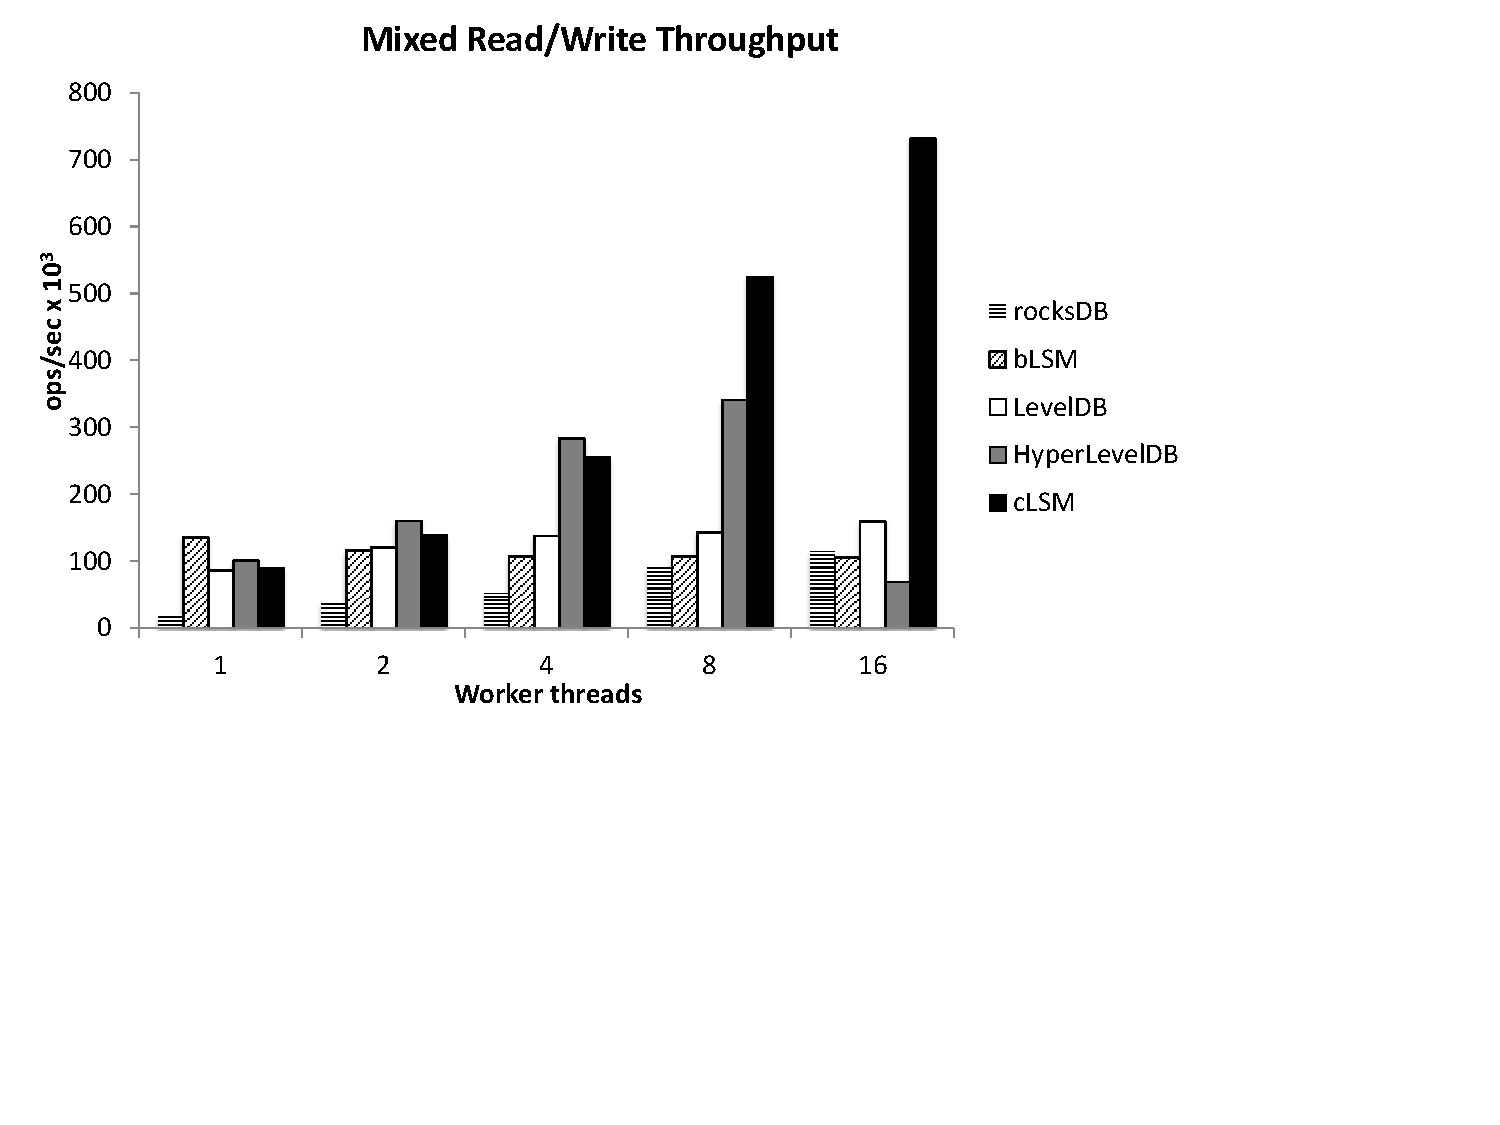
\includegraphics[width=0.9\textwidth,clip, trim =0 180 150 0]{Figures/50r50w_throughput.pdf}}		
		\caption{50\% read, 50\% write}
               \label{fig:50r50w_throughput}
  \end{subfigure}%
%\hspace{0.2\textwidth}
  \begin{subfigure}[t]{0.49\textwidth}
   \center
        \fbox{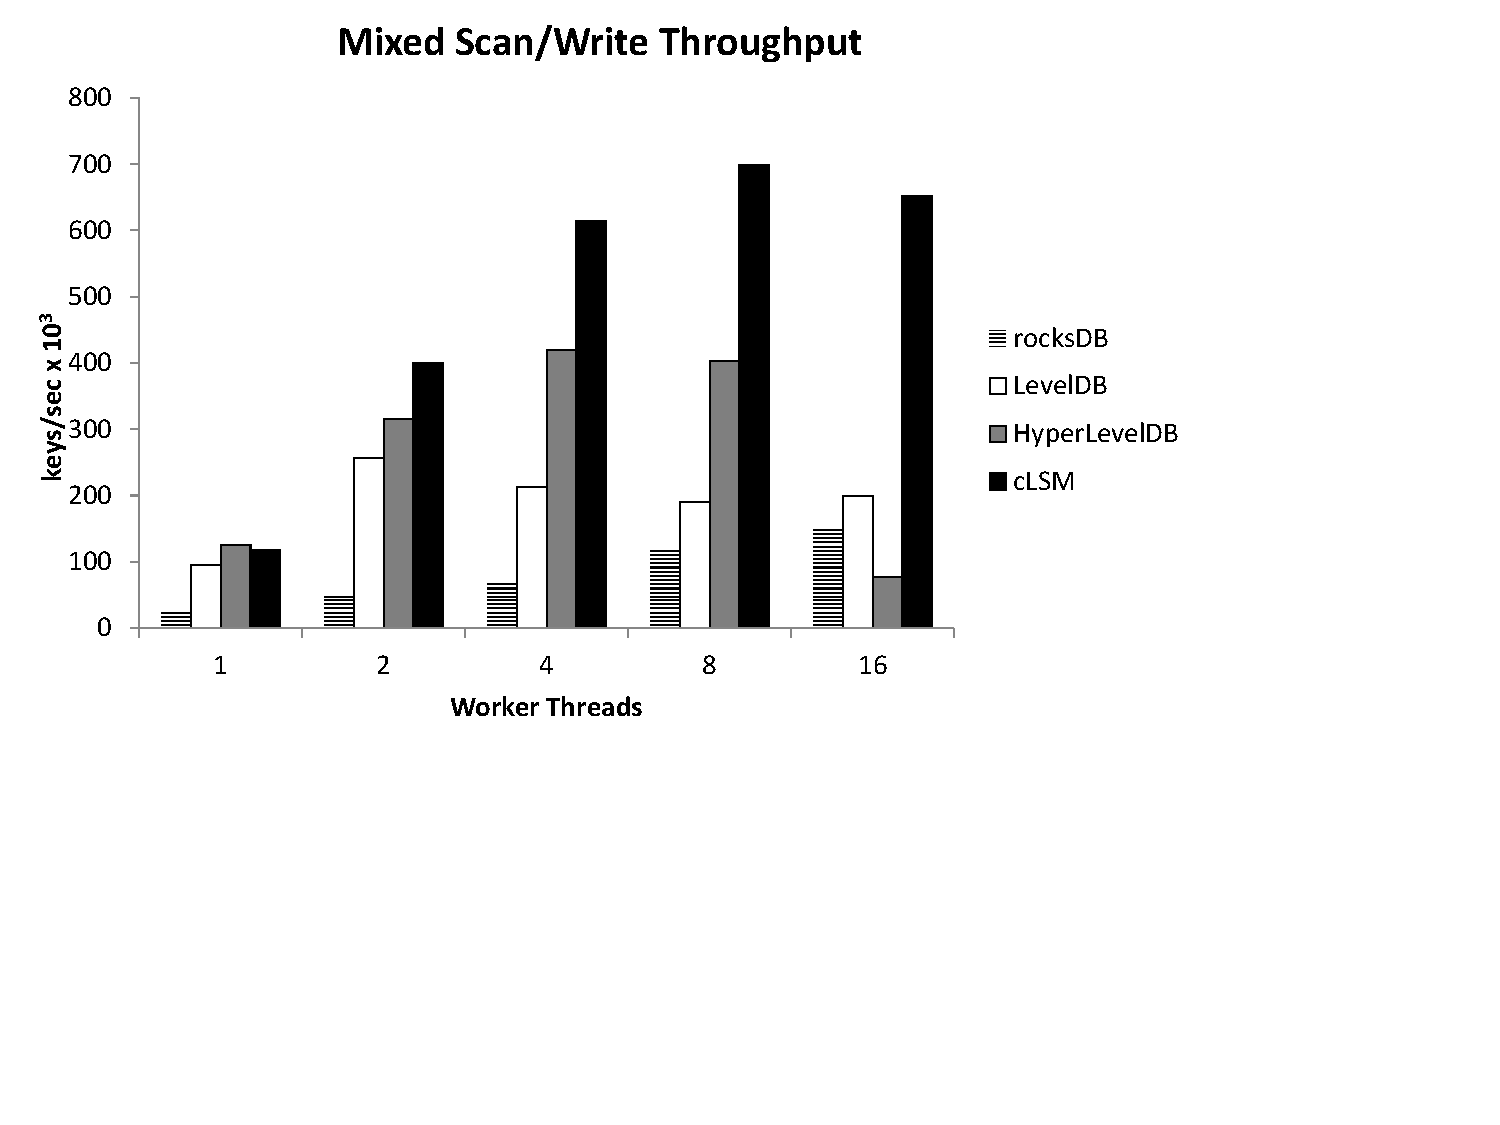
\includegraphics[width=0.9\textwidth,clip, trim =0 180 150 0]{Figures/50scan50w_throughput.pdf}}		
		\caption{50\% scan, 50\% write}
               \label{fig:50scan50w_throughput}
  \end{subfigure}%
\caption{\bf{Throughput in mixed workloads.
%(a) 50\% read/50\% write -- {\clsm}'s peak rate is superior vs the closest competitor by 2.1x. (b) 50\% scan/50\% write --
%{\clsm}'s peak rate (keys per second) is superior by 1.6x.
}}
\label{fig:mixed}
\end{figure*}


We next evaluate how the system may benefit from additional RAM.
%
Figure~\ref{fig:50r50w_buffer} compares {\leveldb}'s and {\clsm}'s benefit from larger memory components,
under the read-write workload, with 8 working threads. {\leveldb\/} performs nearly the same for
all sizes beyond 16MB, whereas {\clsm\/} keeps improving with the memory buffer growing to 512MB.
%This can be explained by the fact that {\clsm} permits several concurrent threads to insert items into the in-memory component,
%whereas in {\leveldb\/} only a single thread may update the in-memory component.
%
%This can be explained as follows.
In general, LSM data stores may gain from increasing the in-memory component
size thanks to better batching of disk accesses~\cite{hbaseRegionArch}. However, this also entails slower in-memory operations. We see that \clsm\ successfully masks this added latency via its high degree of parallelism,
which the less scalable alternatives fail to do.


{\bf {Read-Modify-Write.}}
We now explore the performance of atomic RMW operations (put-if-absent flavor~\cite{shacham2014verifying}).
%None of {\clsm}'s competitors supports the RMW abstraction originally.
To establish a comparison baseline, we augment {\leveldb\/} with a textbook RMW implementation
based on lock striping~\cite{GrayTP1993}. The algorithm  protects each RMW and write
operation with an exclusive granular lock to the accessed key.
The basic read and write implementations remain the same.%, including the concurrency control.

We compare the lock-striped {\leveldb\/} with {\clsm}. The first workload under study is comprised
solely of RMW operations. As shown in Figure~\ref{fig:100rmw_throughput}, {\clsm\/} scales to almost 400K operations/sec -- a $2.5$x
throughput gain compared to the standard implementation.
This volume is almost identical to the peak write load.
%This is explained by  {\clsm}'s high CPU utilization, which allows scaling to 16 threads.
%The median latency with that configuration is 17 {\microsec}, versus {\leveldb}'s 36 {\microsec} (Figure~\ref{fig:100rmw_latency}).


\begin{figure}%[tb]
\centerline{
\fbox{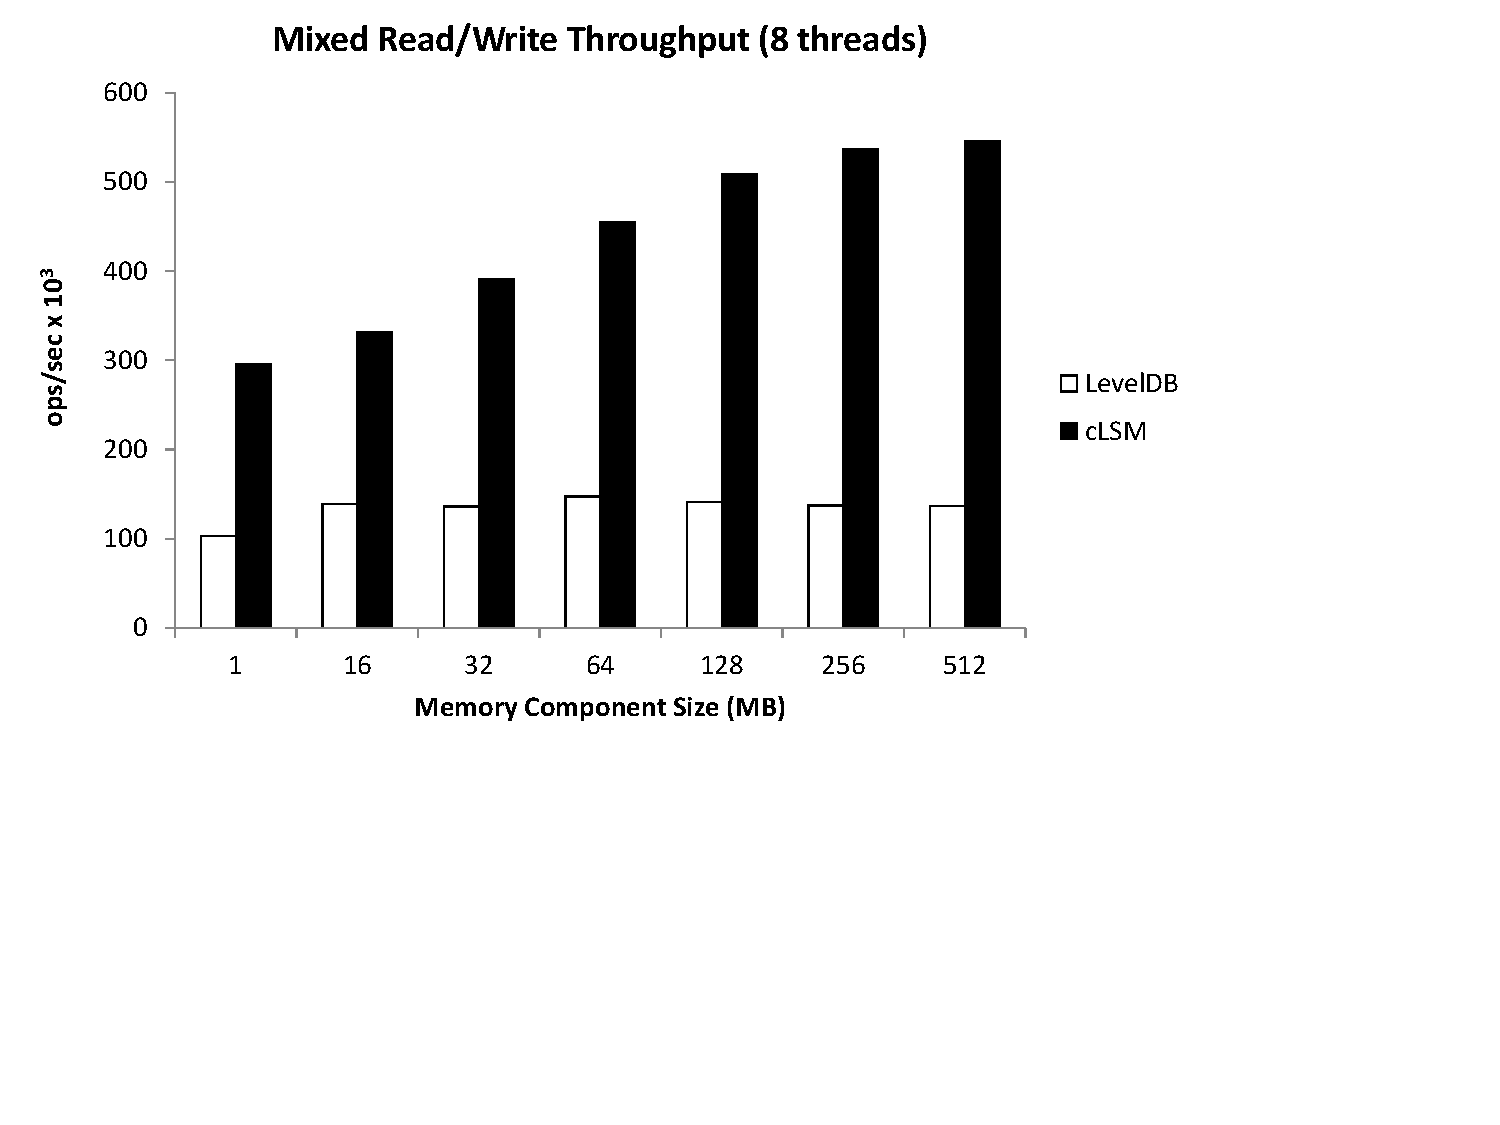
\includegraphics[width=0.45\textwidth,clip, trim =0 180 150 0]{Figures/50r50w_buffer.pdf}}
}
\caption{\bf{Mixed reads and writes benefit from memory component size with 8 threads.
{\clsm\/} successfully exploits RAM buffers of up to 512MB, whereas {\leveldb} can only exploit 16MB. }}
\label{fig:50r50w_buffer}
\end{figure}

\begin{figure}%[tb]
\centerline{
\fbox{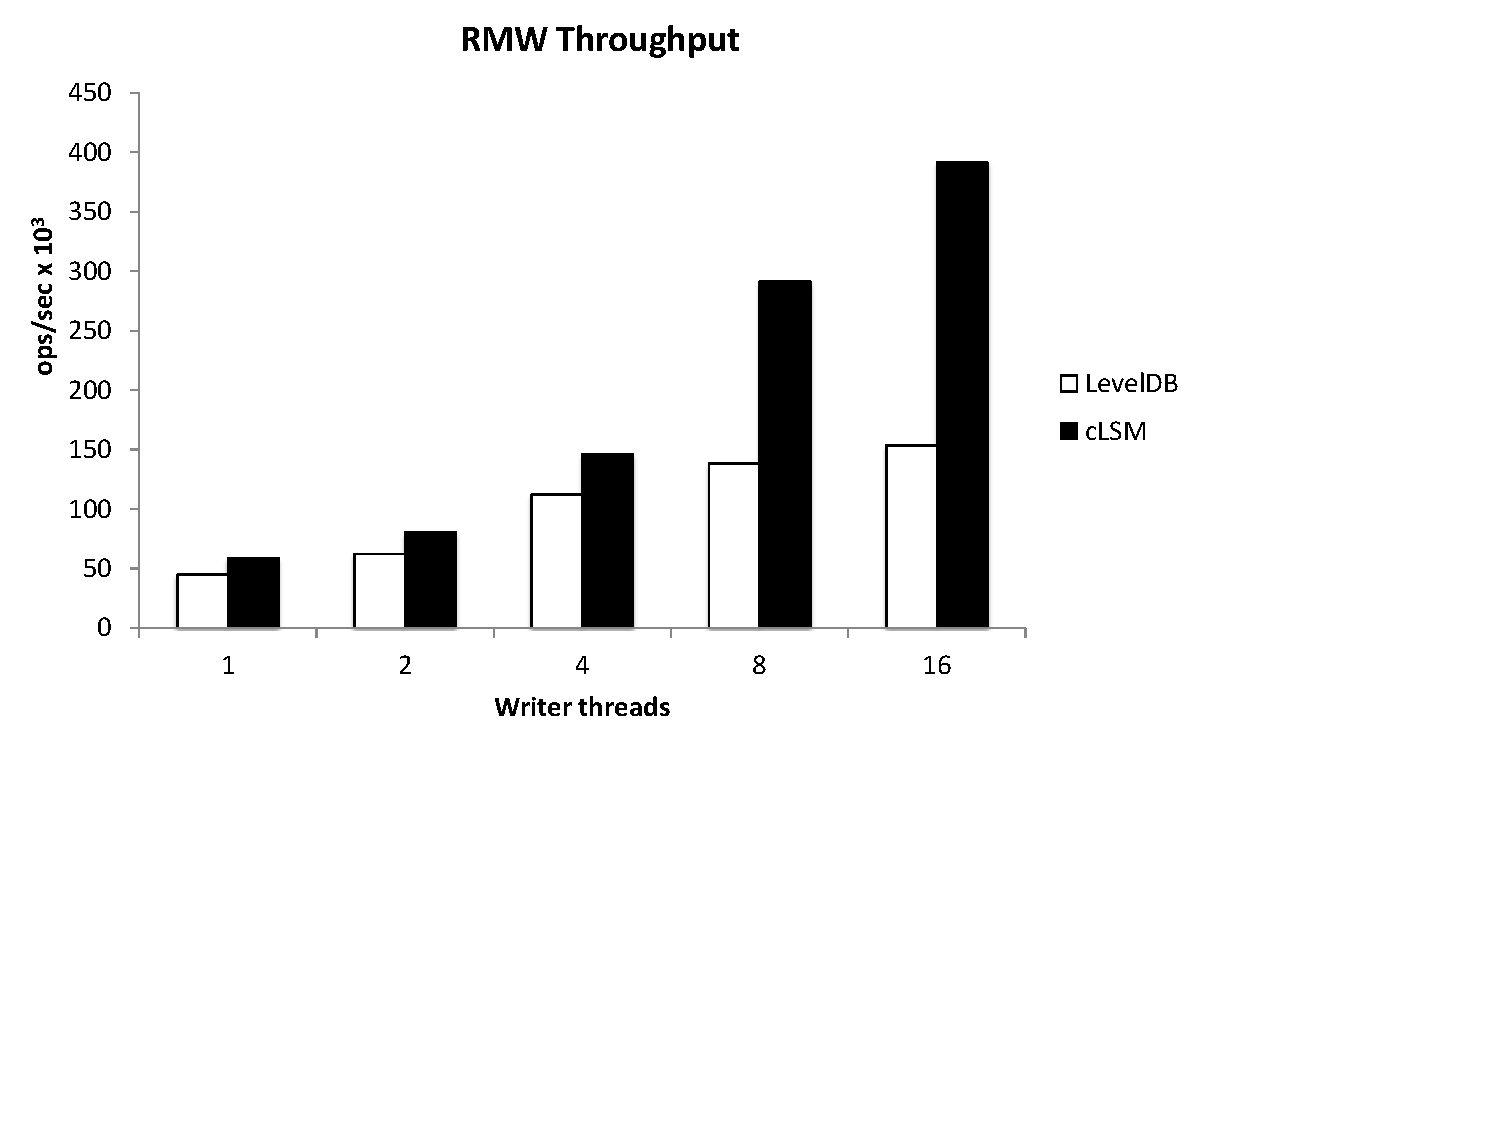
\includegraphics[width=0.45\textwidth,clip, trim =0 180 150 0]{Figures/100_rmw_throughput.pdf}}
}
\caption{\bf{Read-modify-write (RMW) throughput -- a 100\% put-if-absent scenario with locality.
{\clsm\/} improves upon lock-striping by 150\%.}}
\label{fig:100rmw_throughput}
\end{figure}

%\begin{figure*}[tb]
%  \centering
%  \begin{subfigure}[t]{0.49\textwidth}
%   \center
%        \fbox{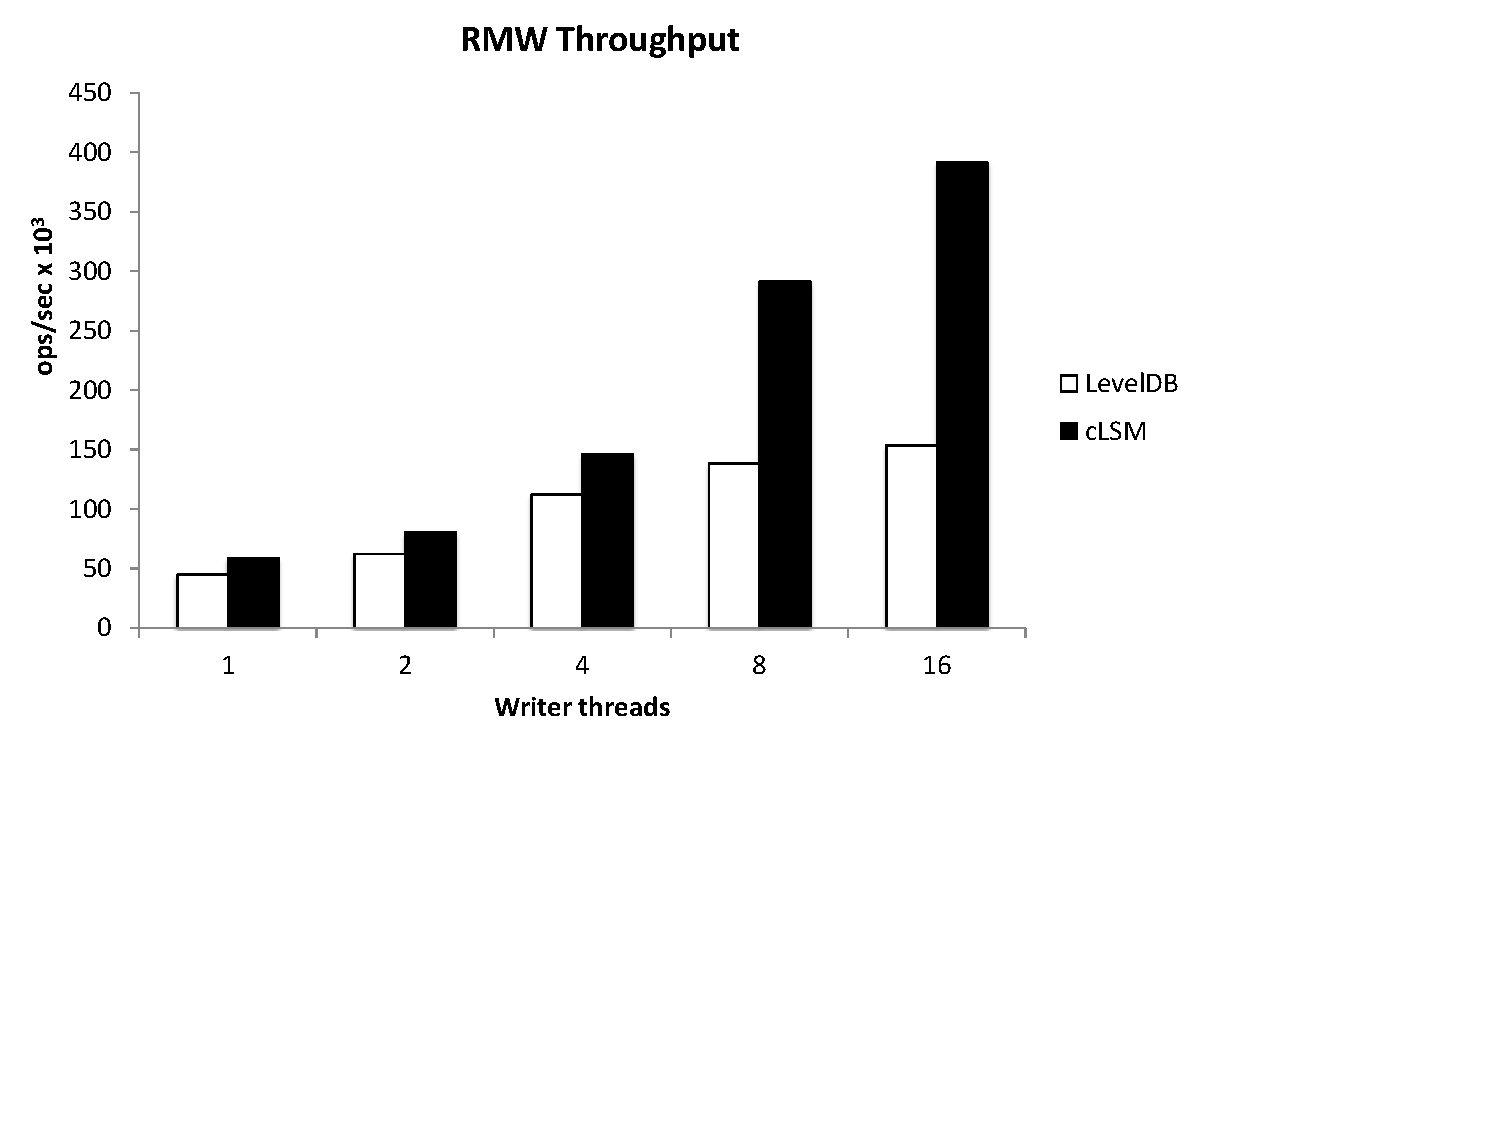
\includegraphics[width=0.9\textwidth,clip, trim =0 180 165 0]{Figures/100_rmw_throughput.pdf}}
%		\caption{Throughput}
%               \label{fig:100rmw_throughput}
%  \end{subfigure}%
%%\quad
% %\hspace{0.2\textwidth}
%  \begin{subfigure}[t]{0.49\textwidth}
%   \center
%		\fbox{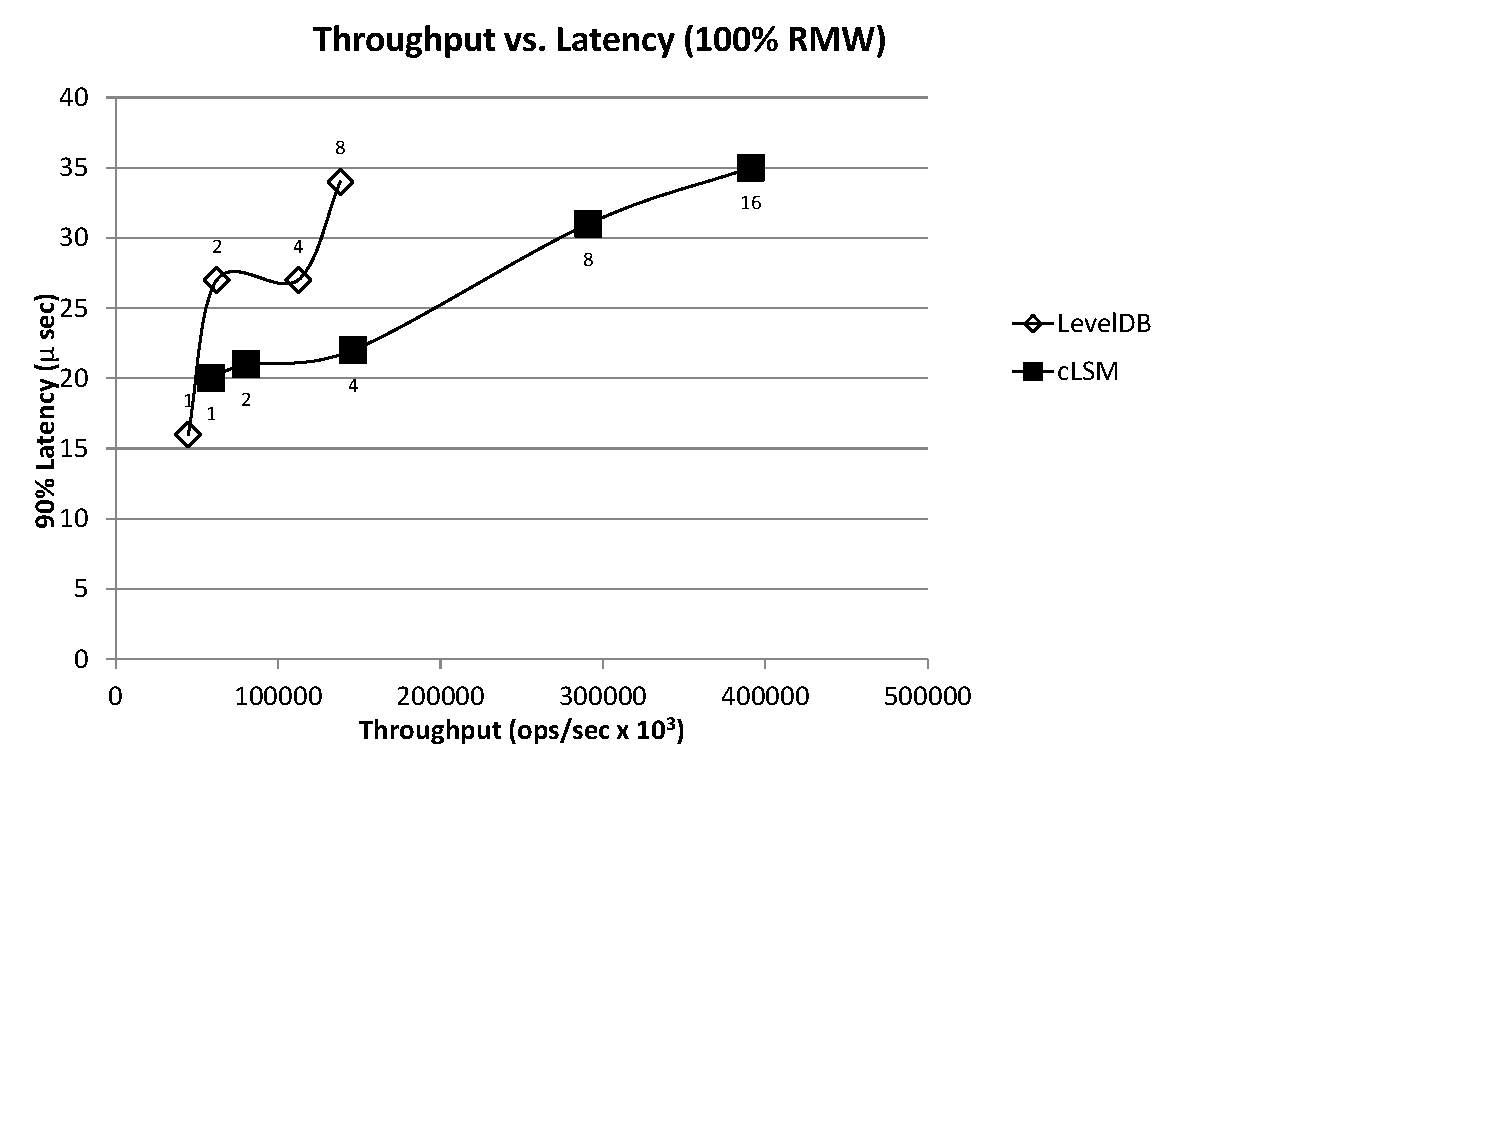
\includegraphics[width=0.9\textwidth,clip, trim =0 180 165 0]{Figures/100_rmw_latency_vs_throughput.pdf}}
%		\caption{Throughput versus Latency}
%               \label{fig:100rmw_latency}
%  \end{subfigure}%
%\caption{\bf{Read-modify-write (RMW) performance -- a 100\% put-if-absent scenario with locality.
%{\clsm\/} exceeds the na\"{\i}ve lock-striping throughput by 150\%, and
%has superior median and 90\% latencies.}}
%\label{fig:100rmw}
%\end{figure*}

%{\bf {Disk Activity.}}
%In the above experiments, the {\clsm} performance can be explained by its effective in-memory synchronization.
%In order to understand the behaviour of the {\clsm}'s disk-component, we measure the amount of time the \emph{compaction procedures} are running
%(as described in Section~\ref{ssec:lsm}, compactions are used to rearrange the internal components of the disk-component).
%Figure~\ref{fig:CompactionsExecution} shows the percentage of execution time in which compactions are running in our experiments.
%The results indicate that, in most cases, compactions are running for at least $50\%$ of the execution time.
%Note that, {\clsm}'s compactions are executed by a single background thread (the implementation of the disk compactions has been taken from {\leveldb}).
%
%\begin{figure}
%\footnotesize
%\begin{tabular}{ c | c }
%%  Workload & Average $\%$ time compaction is running   \\
%  Workload & Average $\%$ time    \\
%           & compactions are running in the background  \\
%  \hline
%  100\% write & 65\%   \\
%  100\% read & 49\%   \\
%  50\% write, 50\% read & 75\%   \\
%\end{tabular}
%\caption{\bf{Execution time of compactions in {\clsm}.}}
%\label{fig:CompactionsExecution}
%\end{figure}



\subsection{Production Workloads}
\label{sec:realworkloads}

\begin{figure*}[tb]
  \centering
  \begin{subfigure}[t]{0.4\textwidth}
   \center
        \fbox{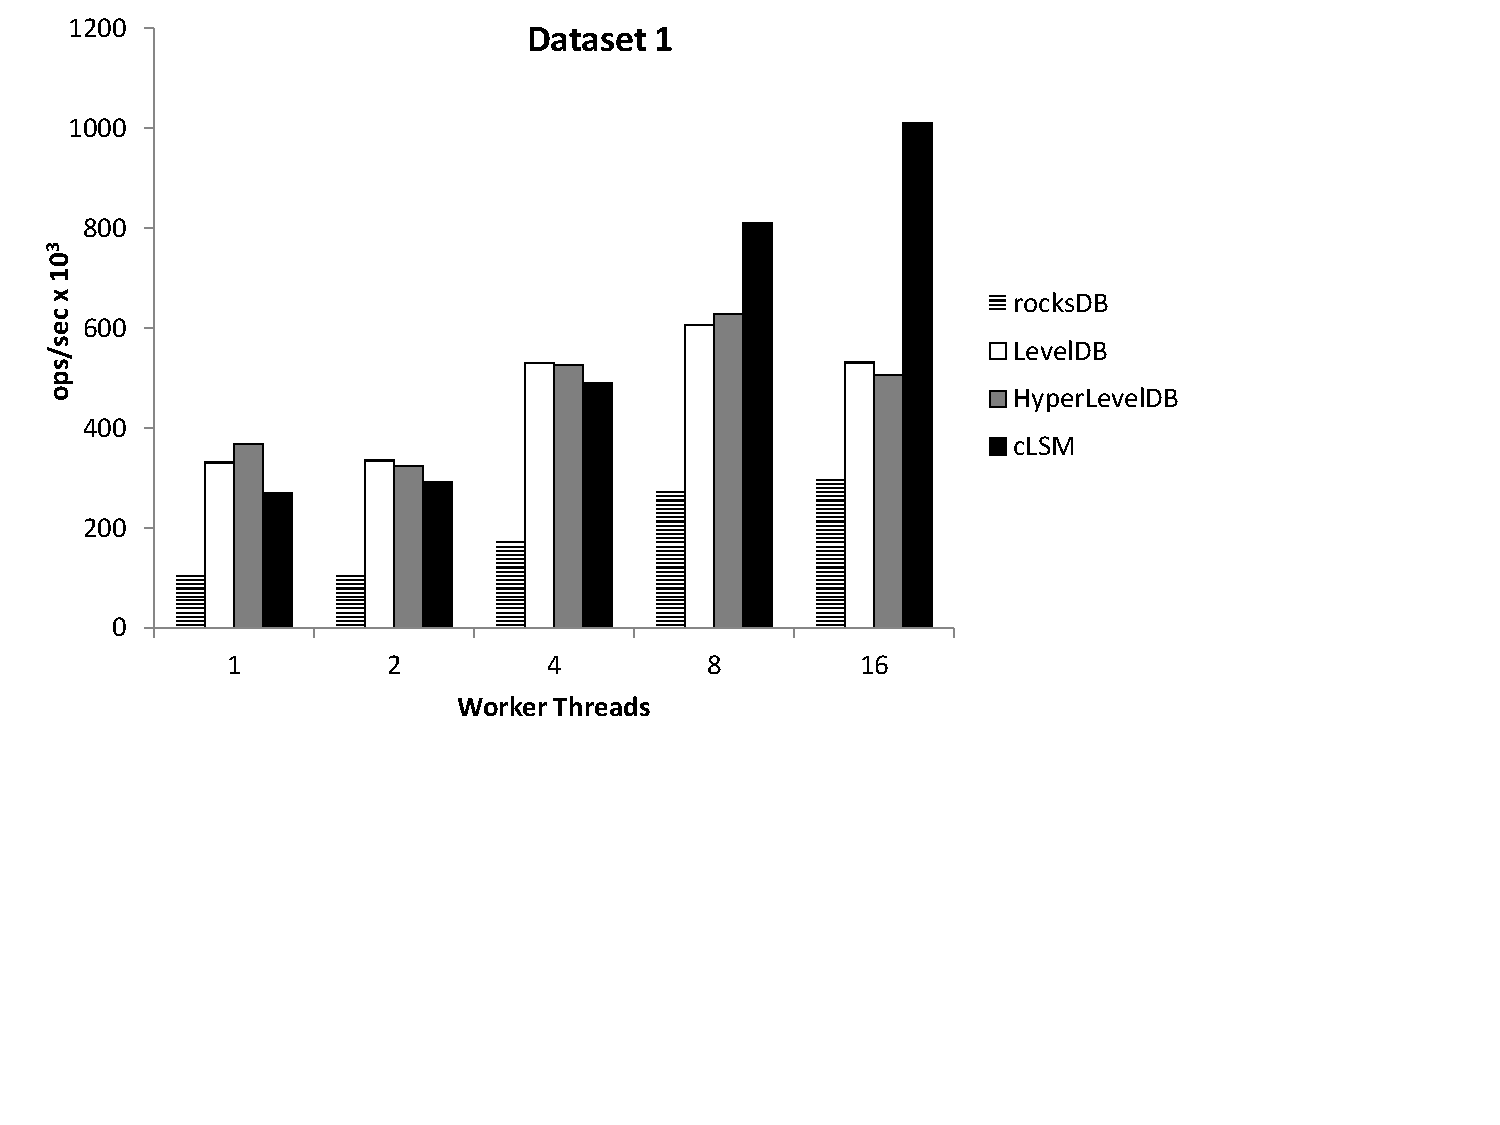
\includegraphics[width=0.9\textwidth,clip, trim =0 180 155 0]{Figures/prodA.pdf}}	
		\caption{93\% reads}
               \label{fig:prodA}
  \end{subfigure}%
%\quad
 %\hspace{0.05\textwidth}
  \begin{subfigure}[t]{0.4\textwidth}
   \center
        \fbox{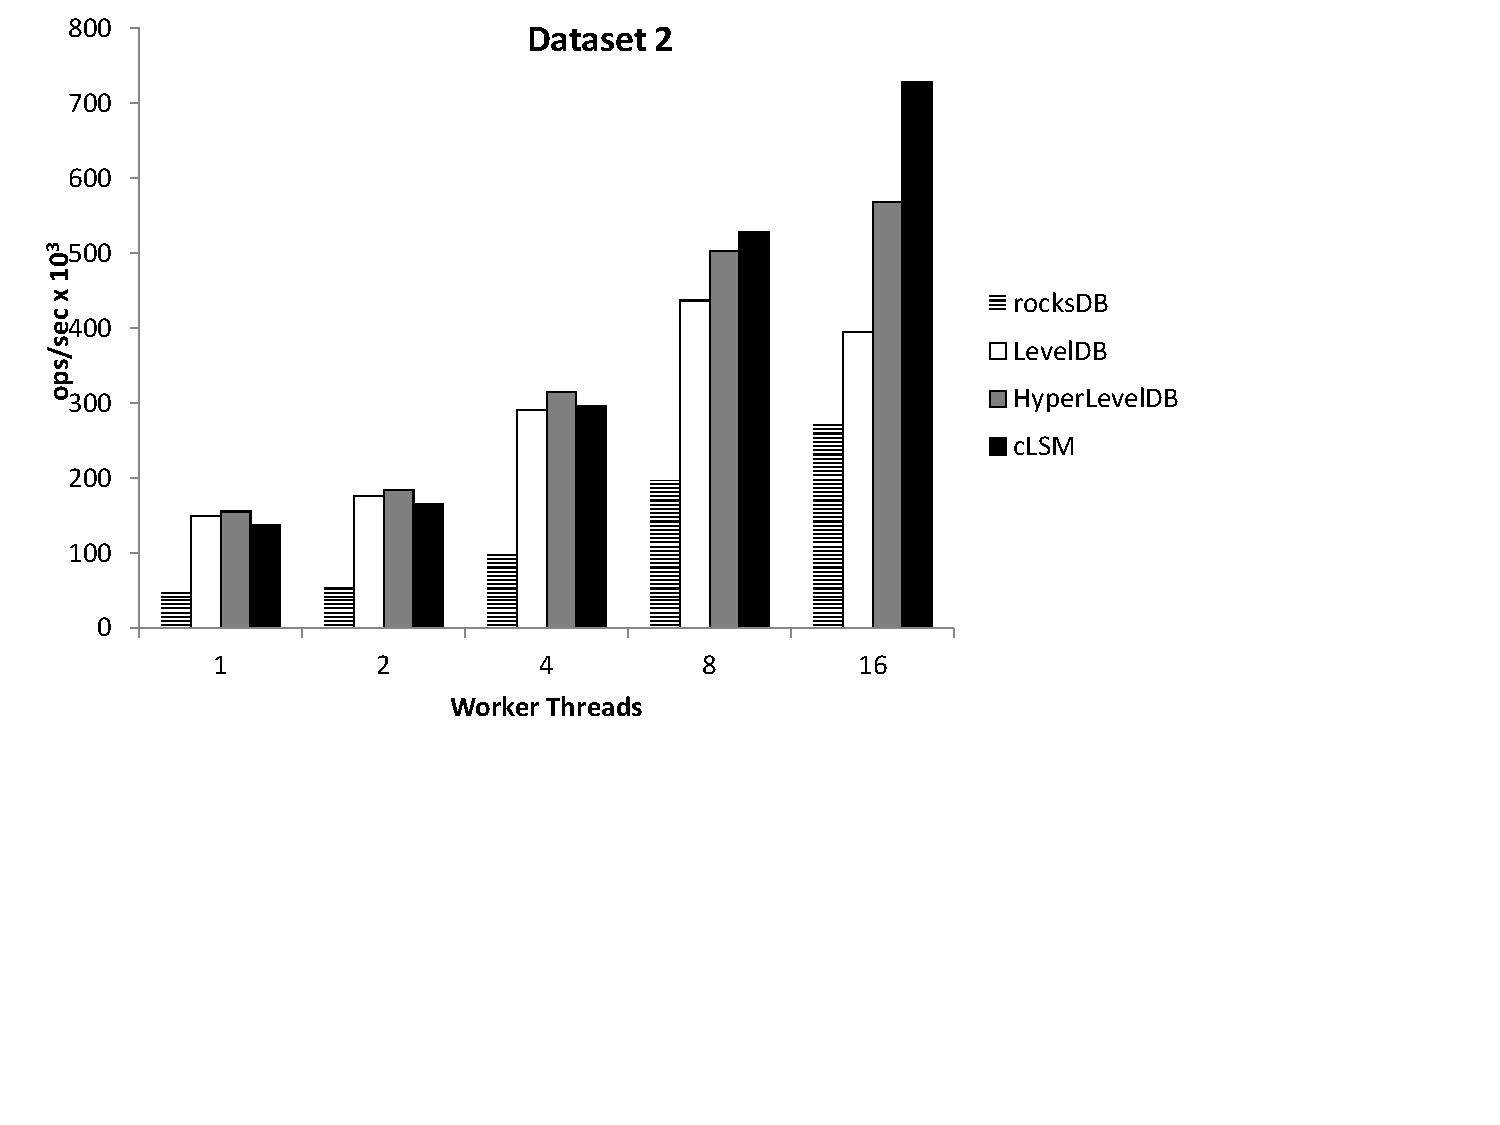
\includegraphics[width=0.9\textwidth,clip, trim =0 180 155 0]{Figures/prodB.pdf}}
		\caption{85\% reads}
               \label{fig:prodB}
  \end{subfigure}%
\hfill
  \centering
  \begin{subfigure}[b]{0.4\textwidth}
   \center
        \fbox{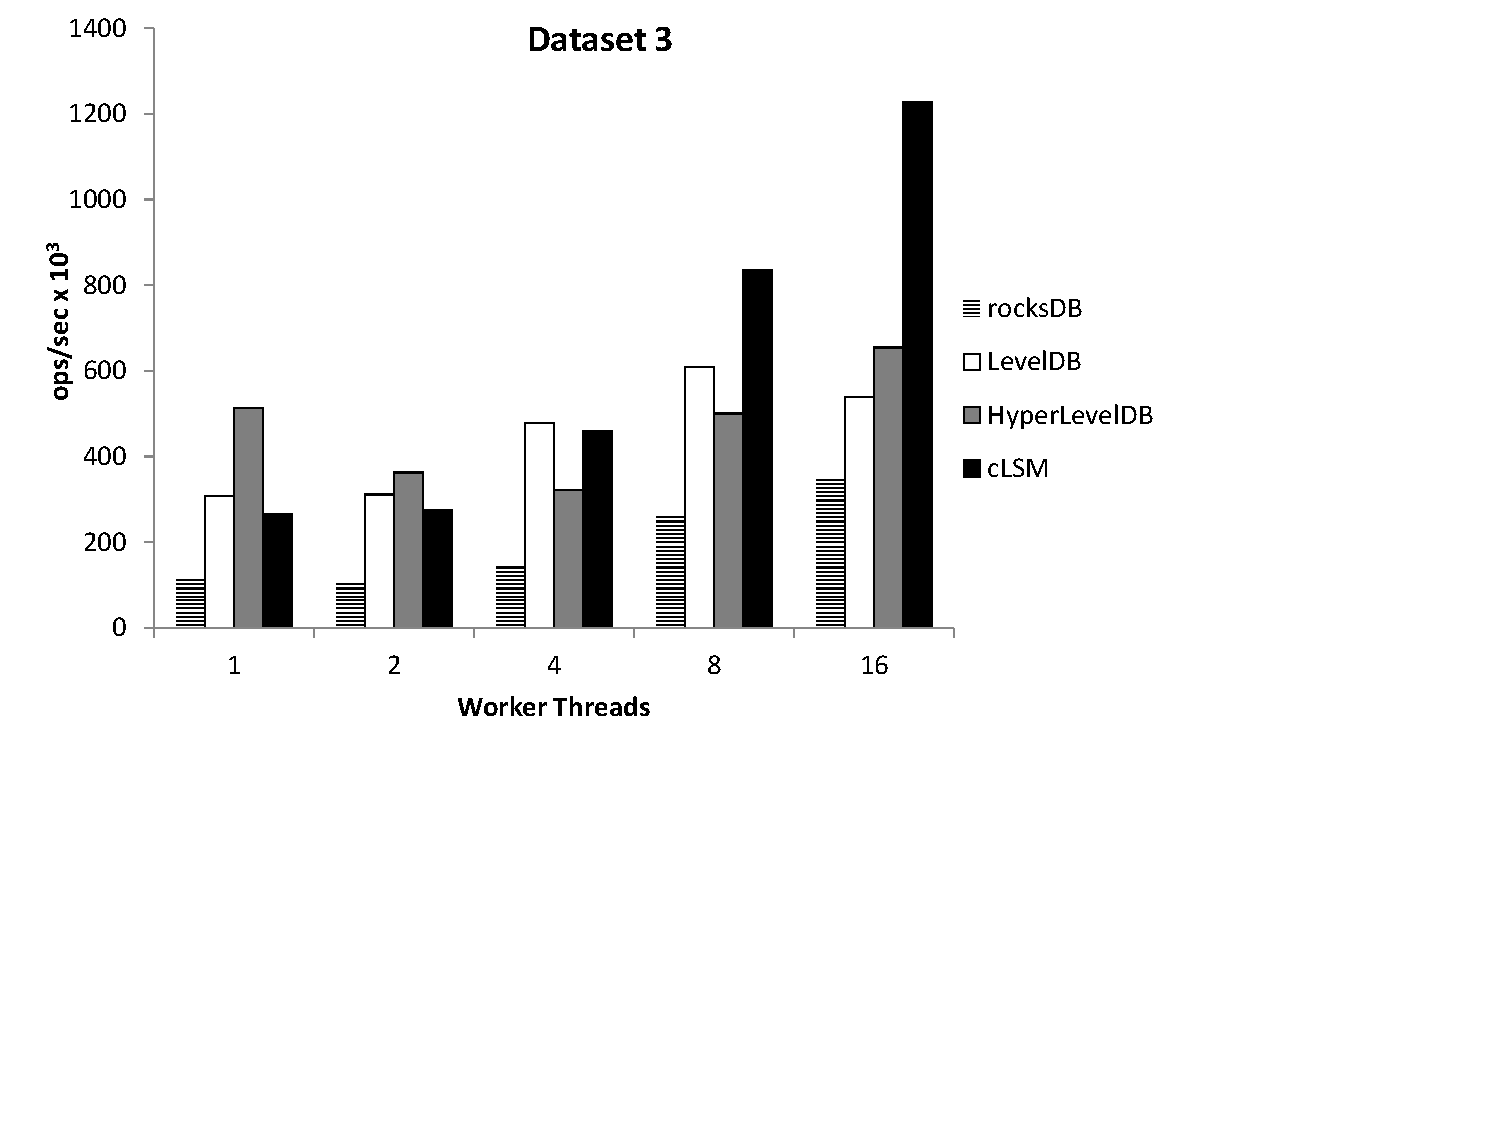
\includegraphics[width=0.9\textwidth,clip, trim =0 180 155 0]{Figures/prodD.pdf}}
		\caption{96\% reads}
               \label{fig:prodD}
  \end{subfigure}%
%\quad
 %\hspace{0.05\textwidth}
  \begin{subfigure}[b]{0.4\textwidth}
   \center
        \fbox{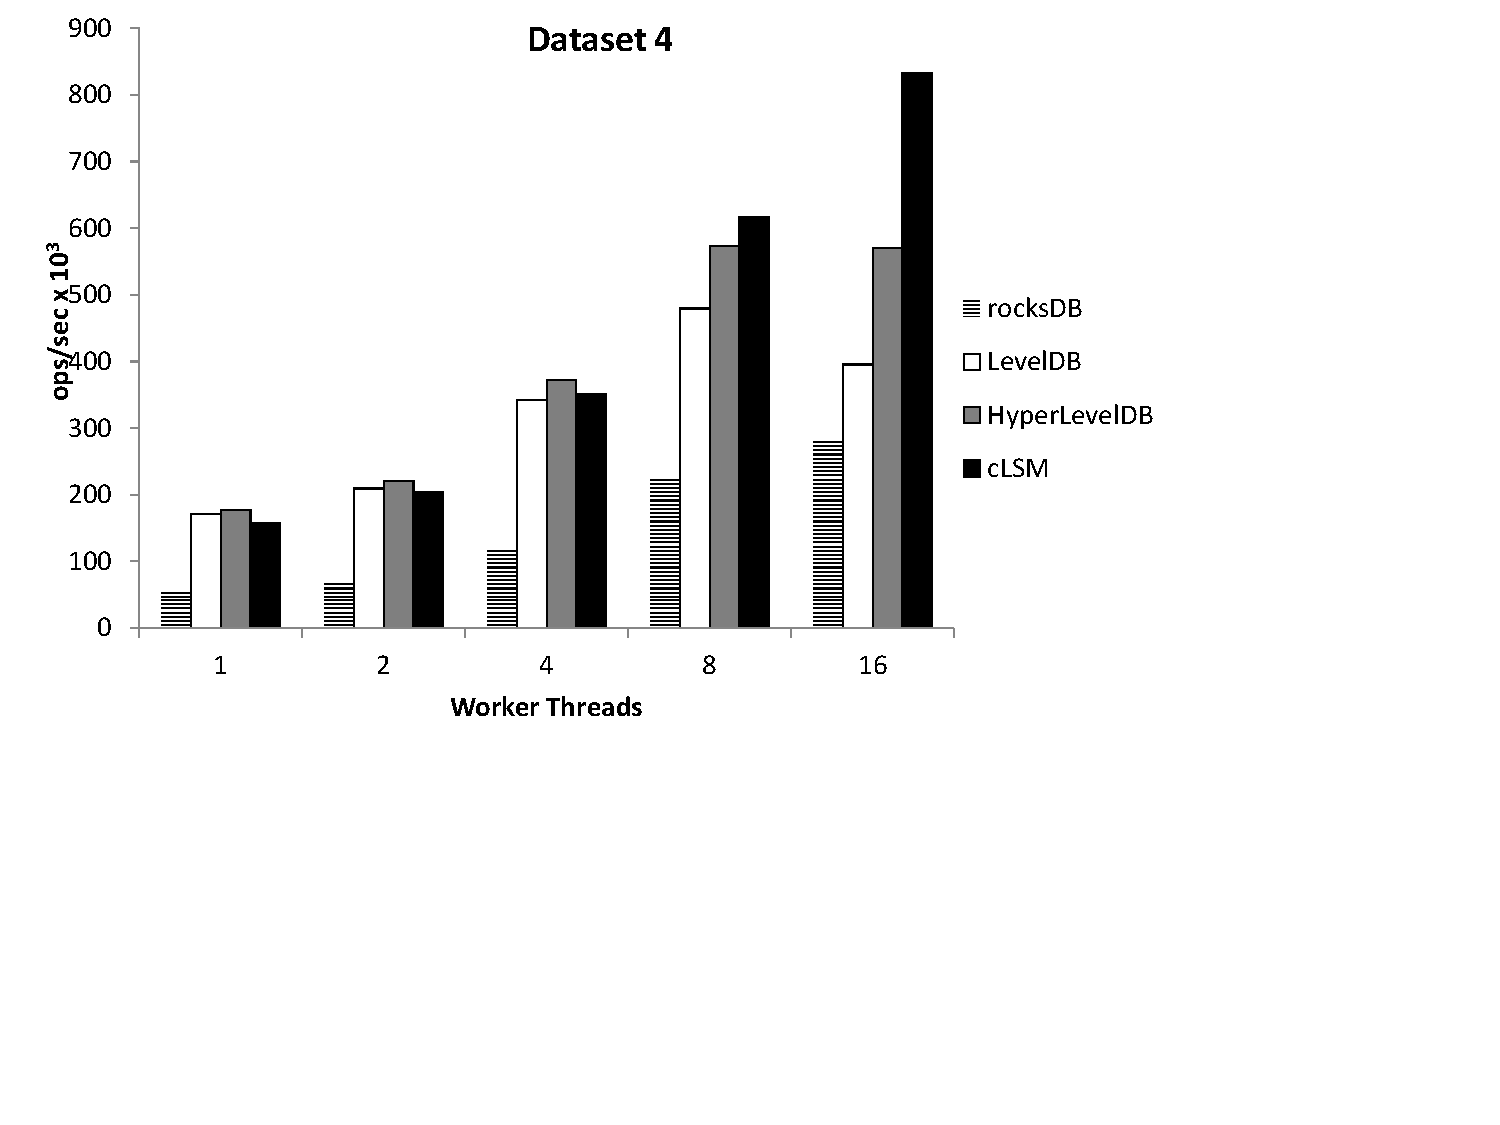
\includegraphics[width=0.9\textwidth,clip, trim =0 180 155 0]{Figures/prodE.pdf}}
		\caption{86\% reads}
               \label{fig:prodE}
  \end{subfigure}%
\caption{\bf{
Throughput in workloads collected from a production web-scale system.
}}
\label{fig:production}
\end{figure*}

We study a set of $20$ workloads logged in a production key-value store that
serves some of the major personalized content and advertising systems on the web. Each log captures the
history of operations applied to an individual partition server. The average
log consists of approximately 5 million operations.
\eurosys{E1}{Operations have variable key and value sizes, averaging $40$-bytes per key, and 1KB
values.} The captured workloads are read-dominated (85\% to 95\% reads).  The key distributions are heavy-tail,
all with similar locality properties. In most settings, 10\% of the keys stand for more than 75\% of the requests,
while the 1-2\% most popular keys account for more than 50\%. Approximately 10\% of the keys are only
encountered once.


Figure~\ref{fig:production} depicts the evaluation results for 4 representative workloads.
Although {\clsm} is slower than the alternatives with a small number of
threads, its scalability is much better.
These results are similar to the results shown in~\ref{fig:50r50w_throughput}.
\eurosys{E1}{However, our advantage over
the competitors is reduced, because, with larger keys and values, the
synchronization overhead is less pronounced.}




\remove{
We also use the logs to conduct an  experiment that compares two approaches to vertical scalability.
We evaluate {\clsm\/} with one big partition versus {\leveldb\/} and {\hyperleveldb\/} with four small partitions.
%Recall that, in many cases, the former setting is more efficient from the I/O perspective~\cite{hbaseRegionArch}.
In this experiment, each small partition
is based on a distinct log, and the big partition is a union thereof.  Each of the small partitions is served
by a dedicated $1/4$ of the thread pool (resource separation), whereas the big partition is served by all
worker threads (resource sharing).
Figure~\ref{fig:production_partitions} depicts the comparison.
We see that {\clsm\/}'s improved concurrency control scales better than partitioning, achieving a peak throughput of above 1 million operations/sec -- approximately 25\% above the competition.
%
This suggests that vertical scalability can sometimes go further than increased horizontal scaling.


\begin{figure}[tbh]
\centerline{
{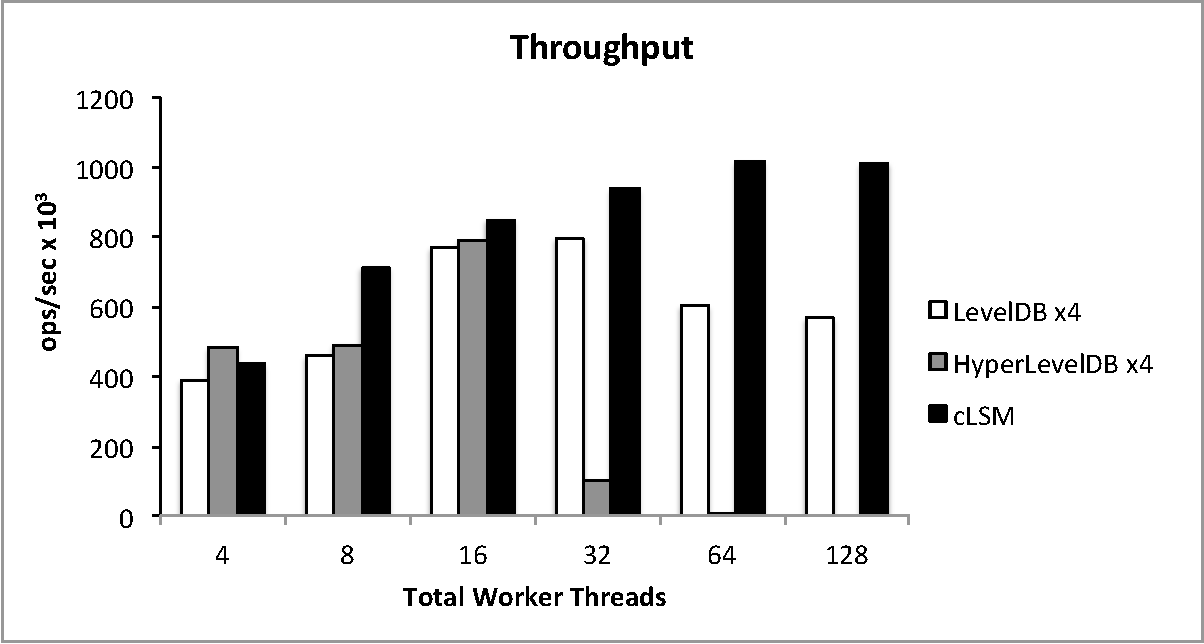
\includegraphics[width=\columnwidth]{Figures/prod4Partitions.pdf}}
}
\caption{\bf{Production workload -- comparing two approaches to vertical scalability.
The resource-isolated configuration exercises {\leveldb\/} and {\hyperleveldb\/} with
4 separate partitions, whereas the resource-shared configuration evaluates {\clsm\/} with
one big partition.
%{\clsm} scales 25\% beyond the competition.
}}
\label{fig:production_partitions}
\end{figure}
}


\subsection{Workloads with Heavy Disk-Compaction}
\label{sec:heavyCompaction}

The above experiments demonstrate situations in which the in-memory access is the main performance bottleneck.
Recently, the {\rocksdb} project has shown that in some scenarios, the main  performance bottleneck is  disk-compaction~\cite{RocksDBBenchmarks}.
%
In these scenarios, a huge number of items is inserted (at once) into the LSM store, leading to many heavy disk-compactions.
As a result of the high disk activity, the  $C_{m}$ component frequently becomes full before the $C_{m}'$ component has been merged into the disk.
This causes client operations to wait until the merge process completes.

We use a benchmark from~\cite{RocksDBBenchmarks} to demonstrate this situation.
In this benchmark, the initial database is created by sequentially inserting 1 billion items.
During the benchmark, 1 billion update operations are invoked by the worker threads.
\eurosys{E3}{As in~\cite{RocksDBBenchmarks}, each key is of size $10$
bytes; however, each value is of size $400$ bytes (instead of $800$)} to ensure that our $720$GB disk is sufficient.


We compare {\clsm} with {\rocksdb} \eurosys{E3}{following the configuration
in~\cite{RocksDBBenchmarks}.
% For {\rocksdb}, we use the configuration in~\cite{RocksDBBenchmarks}.
{\rocksdb} is configured to use multi-threaded compactions so that multiple
threads can simultaneously compact non-overlapping key
ranges in multiple levels.
%For {\clsm}, we adopt part of the {\rocksdb} configuration:
%
%although {\clsm} and {\rocksdb} have different configurable parameters,
%some of these parameters appear in both configurations;
For each parameter that appears both in {\clsm} and {\rocksdb}, we configure the
systems to use the same values.
Specifically, these parameters are: size of
in-memory component ($128$MB), total number of levels ($6$ levels), target file size at level-1 ($64$MB),
and number of bytes in a block ($64$KB).
}

Figure~\ref{fig:HeavyCompactions} depicts the results of this benchmark.
The results show that both {\clsm} and  {\rocksdb}  scale all the way to $16$ worker threads (despite the fact that disk-compaction is running most of the time).
At $16$ threads, {\clsm} becomes equivalent to {\rocksdb}.
Notice that {\rocksdb} uses an optimized compaction algorithm  that utilizes several background threads,
whereas {\clsm} uses a simpler compaction algorithm executed by a single background thread.
It should be noted that {\rocksdb}'s compaction optimizations are orthogonal to our improved parallelism among worker threads.

%\remove{
%eshcar - moved to related.tex for placment
\begin{figure}[t]
\centerline{
\fbox{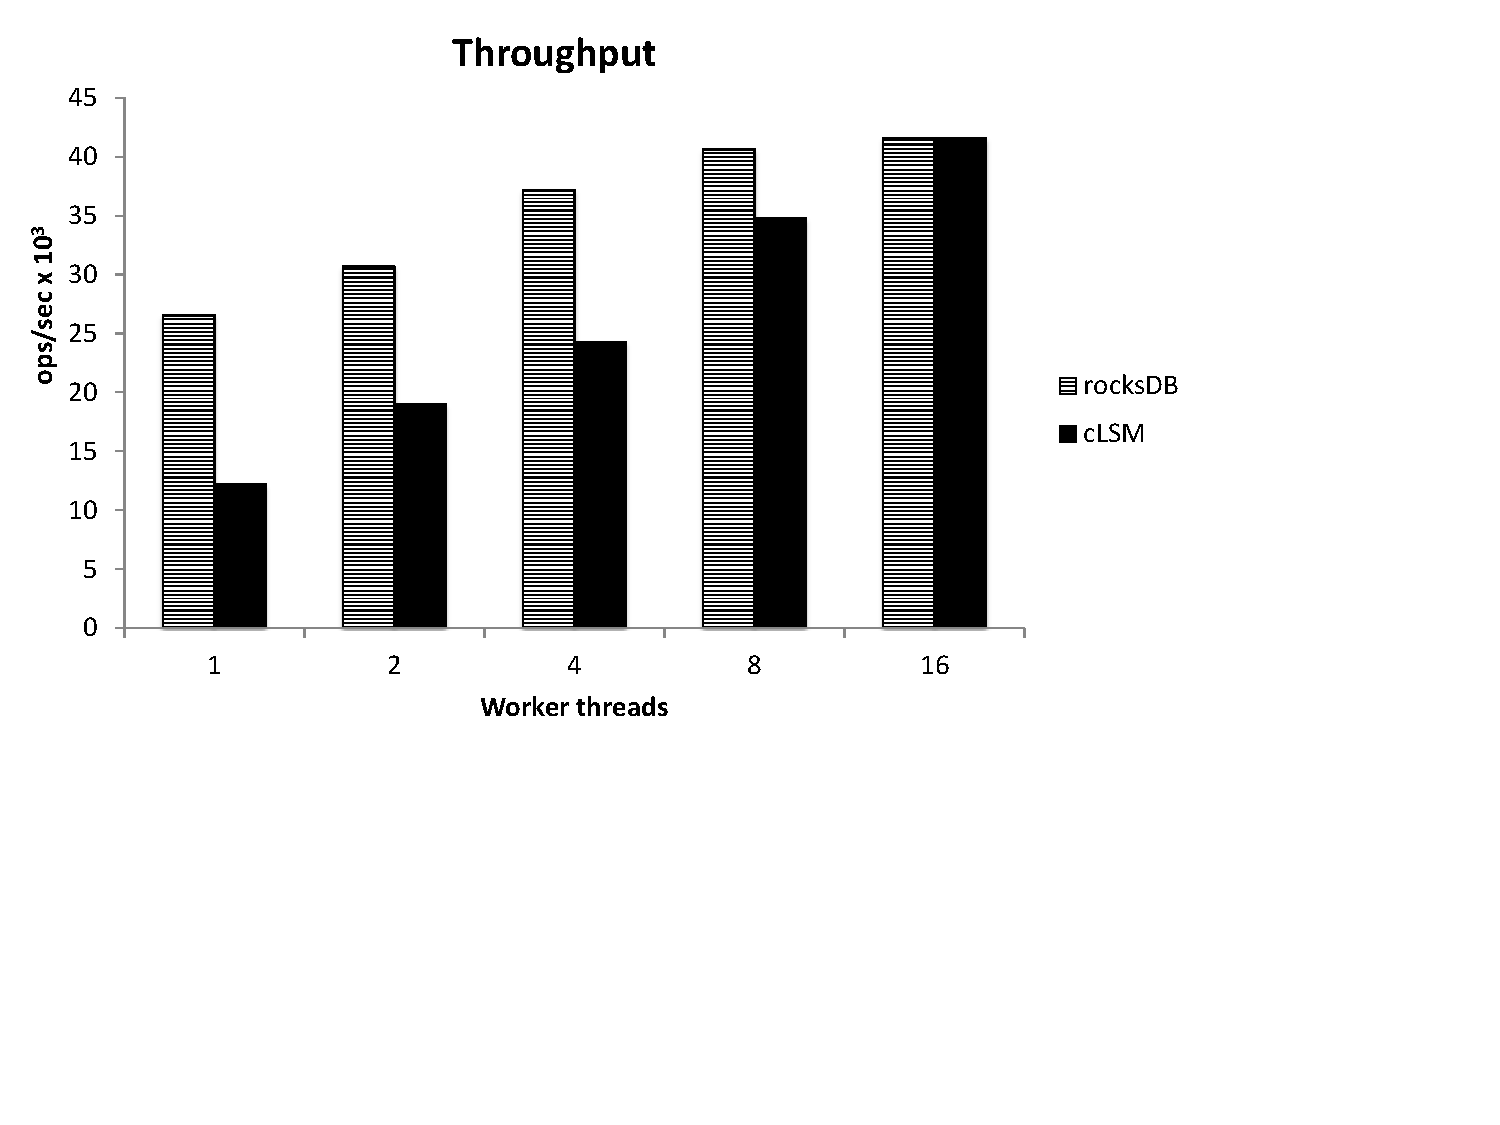
\includegraphics[width=0.45\textwidth,clip, trim =0 180 150 0]{Figures/HeavyCompactions.pdf}}
}
\caption{\bf{Workload with heavy disk-compaction.}}
\label{fig:HeavyCompactions}
\end{figure}
%}





\section{Related Work}
\label{sec:related}


The basis for LSM data structures is the \emph{logarithmic
method} \cite{Bentley79}.
It was initially
proposed as a way to efficiently transform static search structures into dynamic ones.
%
%A \emph{binomial list} structure stored a sequence of sorted arrays, called
%\emph{runs} each of size of power of two. Inserting an element triggers a
%cascaded series of merge-sorting of adjacent runs. Searching an
%element is done by applying a binary search on the runs starting with the
%smallest run until the element is found.

This method inspired the original work on
\emph{LSM-trees}~\cite{O'Neil1996} and its variant for multi-versioned
data stores~\cite{Muth1998}. LSM-trees provide
low-cost indexing for key-value stores with high rates of put operations, by deferring
in-place random writes and batching them into sequential writes. The LSM-tree
indexing approach employs $B^{+}$-tree-like structures as its disk components,
and for the main memory component, an efficient key-lookup structure similar to a
(2-3)-tree or---more common in recent
implementations---a skip-list~\cite{Pugh90}.

Nowadays, key-value stores are commonly implemented as LSM data
stores~\cite{Bigtable2006,PNUTS2008,hbase,Lakshman2010,RocksDB}.
Google's {\leveldb}~\cite{leveldb} is the state-of-the-art implementation of a
single machine LSM that serves as the backbone in many of such key-value stores.
%
It applies
coarse-grained synchronization that forces all puts to be executed sequentially,
and a single threaded merge process. %, which causes frequent write-stalls.
These two design choices
significantly reduce the system throughput in multicore environment.
This effect is mitigated by {\hyperleveldb}~\cite{HyperLevelDB},  the data storage engine that powers
HyperDex~\cite{Hyperdex2012}. It improves on {\leveldb} in two key ways:
(1) by using fine-grained locking to increase concurrency, and (2) by using a
different merging strategy. Our evaluations show that {\clsm} outperforms both
of them.

\remove{
\begin{figure}[t]
\centerline{
\fbox{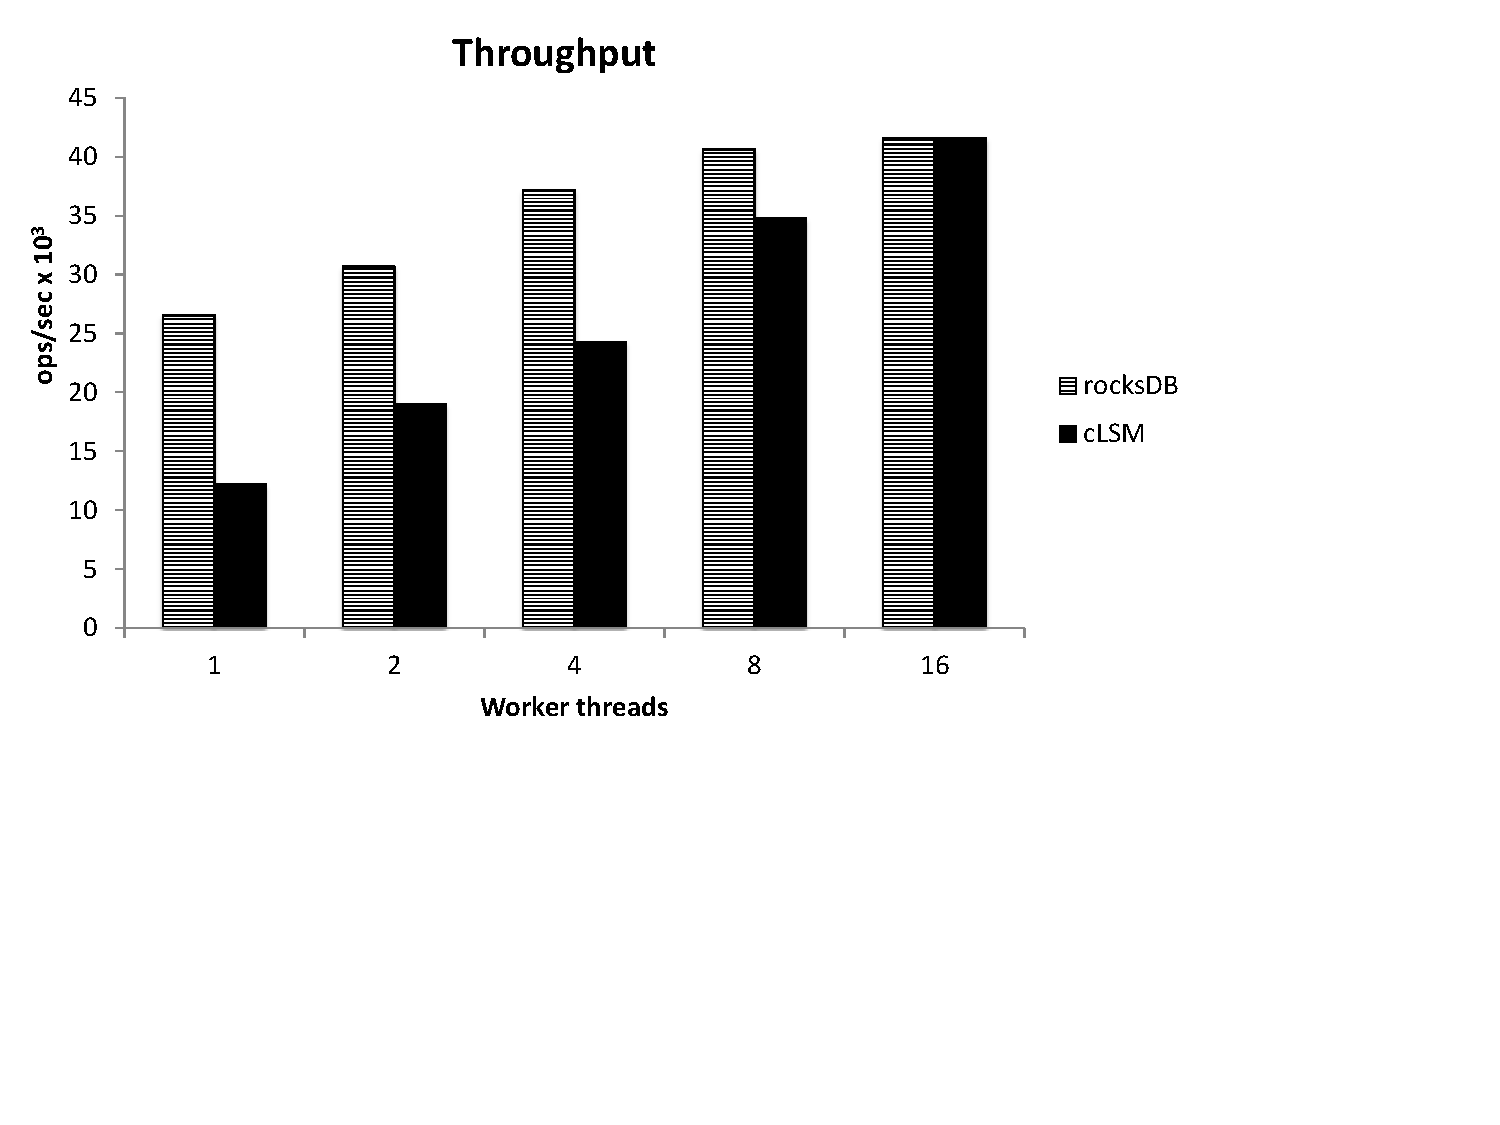
\includegraphics[width=0.45\textwidth,clip, trim =0 180 150 0]{Figures/HeavyCompactions.pdf}}
}
\caption{\bf{Workload with heavy disk-compaction.}}
\label{fig:HeavyCompactions}
\end{figure}
}

Facebook's key-value store, RocksDB~\cite{RocksDB} also builds on {\leveldb}.
%Its memory component supports a single writer and multiple readers.
Much
effort is done in order to reduce critical sections in the memory
component~\cite{RocksDBReduceLocks, RocksDBOptimizedLocks}.
Specifically, readers avoid locks by caching metadata in their thread local storage. Only when a newer
version becomes available readers use locks to get hold of a reference to it.
In addition, the merge process of disk components is executed by multiple
threads concurrently, and some thread is always reserved for flushing the memory
component to the disk.%, thereby avoiding write-stalls.
%RocksDB also supports a basic operator that allows applications to efficiently execute read-modify-write operations.

% bLSM
In the same vein, {\blsm}~\cite{BLSM2012}
introduces a new merge scheduler,
which bounds the time a merge can block write operations.
%In addition, {\blsm}
%leverages Bloom filters~\cite{Bloom1970} to reduce the number of seeks
%(random reads). This results in accelerating searches of items that are not stored in the
%database -- mostly important when invoking an \emph{insert if not
%exists} operation.
As {\blsm} optimizations focus on the merging process and disk
access, it is orthogonal to our work on memory optimizations.



Several approaches for optimizing the performance of the general
logarithmic method have been proposed in recent years.
%
% FD
One such approach suggests adopting a new tree-indexing data structure,
\emph{FD-tree}~\cite{Li2010}, to better facilitate the properties of
contemporary flash disks and solid state drives (SSDs). Like components in LSM-trees, FD-trees maintain multiple
\emph{levels} with cross-level pointers. This approach applies
the \emph{fractional cascading}~\cite{Chazelle86} technique to speed up search
in the logarithmic structure.
%
\remove{
FD-trees aim to (1) minimize the number of
random writes as well as (2) limit them to a small neighborhood, while (3)
preserving high search efficiency. Like the components in LSM-trees, FD-trees
maintain multiple \emph{levels}. Random writes transform into sequential writes
that are initially performed on the top level, and then gradually migrated to
lower levels in batches. The main difference is that instead of having an index
structure at each level (as is the case in LSM components) a level in an
FD-tree holds cross level pointers called \emph{fences} within the sequence of
sorted key entries.
A fence points to a location within the
next level, such that the range between two consecutive fences in level $i$
spans the key range within the page in level $i+1$ that is pointed by the first fence. Essentially,
the cross levels pointers projected by the fences of levels $0\ldots i$ capture
an indexing structure for level $i+1$. Maintaining this implicit structure allows FD-trees
to achieve all 3 properties mentioned above.
}
% FD+
A follow-up work~\cite{FDPlus2012} further refines FD-trees to support
concurrency,  allowing concurrent reads and writes during ongoing index
reorganizations.
\remove{ thus improving both latency and throughput.
The main idea is that a merge of levels $0\ldots m$ progress as a
wavefront within these $m+1$ level. Each level is partitioned into its prefix -- already processed, and yet unprocessed suffix.
The two parts of each level always reflect a single coherent structure. At the
same time, writes are applied to the processed part of the top level, and reads
check the wavefront fence to determine which part of the level to search in.
Blocks in the unprocessed parts are reclaimed only when no new read can go
through them. The top level, which is stored in memory uses a single lock to
control its access. Disk-resident levels use a multi-readers-single-writer lock
per block.
}

With a similar goal of exploiting flash storage as well as the caches of modern
multi-core processors, \emph{Bw-tree}~\cite{LevandoskiLS13} is a new
form of a B-tree, used as an index for a
persistent key-value store.
%To best exploit main memory
The
implementation is non-blocking, allowing for better scalability (throughput). It
also avoids cache line invalidation thus improving cache performance (latency).
Instead of locks, their implementation, which bares similarity to B-link
design~\cite{Lehman1981}, uses CAS instructions, and therefore blocks only
rarely, when fetching a page from disk.
\remove{Attaching delta updates to nodes instead of
performing update-in-place reduces cache invalidation, and thus increases hit
rate.}
At its storage layer, Bw-tree uses log structuring~\cite{RosenblumO1992}.
\remove{It
enables writing large buffers by posting page delta changes, which are
consolidated during a flash cleaning process. Log-structured file system~\cite{RosenblumO1992} is also known to be the source of inspiration
for writing large multi-page blocks to new locations in LSM-trees.
}


%\eshcar{Discuss why our approach is better or explain why we do not compare to
% these solutions. Specifically Bw-tree claims to outperform in-memory
% skip-list.}
None of these new approaches support consistent scans or an atomic RMW
operation (as {\clsm} does). In addition, each of these algorithms builds upon a specific data structure as its
main memory component,
whereas our work can employ any
implementation of a concurrent sorted map to support the basic API.

% % bLSM
% A different approach is presented by {\blsm}~\cite{BLSM2012}. This work
% %improves log structured indexes performance by
% introduces a new merge scheduler,
% which bounds the time a merge can block write operations.
% \remove{The merge process
% ensures that when a component fills, some space becomes available at the next
% component. This significantly reduces the need to block writes to upper levels
% and specifically to $c_0$.
% }
% In addition, {\blsm}
% leverages Bloom filters~\cite{Bloom1970} to reduce the number of seeks
% (random reads). This results in accelerating searches of items that are not stored in the
% database -- mostly important when invoking an \emph{insert if not
% exists} operation.
% \remove{Each disk component is associated with a Bloom filter that
% efficiently represent the items stored in the component with $1\%$ false
% positive rate. This results in each read operation executing $1.03$ seeks in
% expectation, and in accelerating searches of items that are not stored in the
% database. The latter is mostly important when invoking an \emph{insert if not
% exists} operation.
% Bloom filters do not improve scan performance. To address this issue {\blsm}
% choose to bound the number of on-disk components to $3$.
% }
% As {\blsm} optimizations focus on the merging process and disk access, it is
% orthogonal to our work on memory optimizations. We believe the
% two approaches can be combined.


\section{Discussion}
\label{sec:discussion}

Leading key-value stores today rely on LSM-DS methodology for serving requests mostly from RAM.
With this approach, the implementation of in-memory building blocks is critical for performance, as we have demonstrated in Section~\ref{sec:eval}.
The primary challenge such systems face is scaling up with the available hardware resources – most notably, the number of CPU cores.
In this context, the concurrency control that protects shared data structures can be a major performance roadblock.
Our work overcomes this roadblock and presents \clsm, an efficient concurrent LSM-DS implementation.
Scalability is achieved  by eliminating blocking  in scenarios that do not involve physical access to disk.
%Scalability is achieved  by eliminating blocking  in all scenarios that do not involve access to disk.

In addition to atomic reads and writes, \clsm\ supports consistent snapshot scans, range queries, and atomic read-modify-write operations.
Our algorithm is generic, and can be applied to a range of  implementations. Such decoupling allows our solution to be
combined with other optimization applied to the disk components and merge utility.


Our evaluation versus state-of-the-art LSM implementations shows performance improvements and superior scalability,
even when the competitors utilize smaller partitions. The latter, along with other disadvantages of partitioning discussed
in Section~\ref{sec:background}, suggests that our approach can potentially serve as an alternative for vertical scalability.


%The implementation of in-memory building blocks is critical for the
%performance of LSM-DS (as demonstrated in Section~\ref{sec:eval}). The primary challenge is scaling up with the available
%hardware resources -- in particular, the number of CPU cores.
%Similar to all systems that capitalize on internal parallelism, the concurrency control
%that protect the shared data structures is either a major
%performance roadblock or requires nontrivial mechanisms to guarantee the
%overall correctness of the system.
%In this work, we present an efficient concurrent LSM-DS implementation. It features atomic reads and
%writes, snapshots, iterators and an additional atomic read-modify-writes. Our algorithm is
%non-blocking in scenarios that do not involve access to disk.
%The algorithm for supporting the basic key-value store API is generic and can be
%applied to any implementation that does not exploit concurrency.
%Furthermore, this decoupling allows our solution to be combined with
%other optimization that are applied to the disk components and merge utility.
%
%Our evaluation versus state-of-the-art LSM implementations show performance
%improvements and superior scalability, even when the competitors utilize
%smaller partitions. This suggest that our concurrent algorithm can serve as an
%alternative for gaining vertical scalability.


%\subsection*{Acknowledgements}
Omitted for blind review.

\bibliographystyle{acm-nice}
\bibliography{clsm}

%{\small{
%\bibliographystyle{abbrv}
%\bibliography{clsm}
%}}

\end{document}
